%%This is a very basic article template.
%%There is just one section and two subsections.
\documentclass[12pt, oneside]{book}
\usepackage{iitbtitle}
\usepackage[font={small,it}]{caption}
\usepackage{textcomp}
\usepackage{subcaption}
\usepackage{a4wide}
\usepackage{multirow}
\usepackage{anysize}
\usepackage{iitbcs}
\usepackage{latexsym}
\usepackage{amssymb}
\usepackage{amsmath}
\usepackage{graphicx}
\usepackage{epsfig}
\usepackage{comment}
% \usepackage{psfig}
\usepackage{tabls}
\usepackage{multirow} 
\usepackage{tabularx}
\usepackage{url}
\usepackage{nccmath}
\usepackage{textcomp}
\usepackage{mathtools}
\usepackage{etoolbox}% http://ctan.org/pkg/etoolbox
\makeatletter
\patchcmd{\@makechapterhead}{\vspace*{50\p@}}{}{}{}% Removes space above \chapter head
\patchcmd{\@makeschapterhead}{\vspace*{50\p@}}{}{}{}% Removes space above \chapter* head
\makeatother
\usepackage[pagebackref=true,breaklinks=true,colorlinks,bookmarks=false]{hyperref}
\newcolumntype{Y}{>{\centering\arraybackslash}X}
\setlength{\floatsep}{20pt plus 2pt minus 2pt}
\setlength{\textfloatsep}{20pt plus 2pt minus 2pt}
\setlength{\intextsep}{5pt plus 2pt minus 2pt}
\usepackage{color}


\marginsize{2.5cm}{2.5cm}{1cm}{1.5cm}
\def\baselinestretch{1.15}

\newcommand\INPUT{\item[\textbf{Input:}]}
\newcommand\OUTPUT{\item[\textbf{Output:}]}
\providecommand{\norm}[1]{\lVert#1\rVert}
\DeclareGraphicsExtensions{.pdf,.png,.jpg}
\DeclareRobustCommand\onedot{\futurelet\@let@token\@onedot}
\def\etal{\emph{et al}\onedot}
\begin{document}
%\baselineskip 20pt
%The definitions
\def\title{Exploration of Multiplanar Scenes through Autonomous Navigation of
Quadcopter} 
\def\degree{Doctor of Philosophy}
\def\who{Meghshyam G. Prasad}
\def\roll{124058001}
\def\guide{Prof. Sharat Chandran}
\titlpage
\def\bsq{\begin{flushright} $\blacksquare$\\ \end{flushright}}
\def\tab{\hspace{5mm}}
\pagenumbering{roman}
\chapter*{Acknowledgements}
I express deep and sincere gratitude to Prof. Sharat Chandran and Prof.
Michael Brown for providing constant direction and guidance.  I take this
opportunity to thank Mr. Anirudh Vemula for his help in path planning work. I
am also thankful to Mr.Sona Praneeth Akula for his help in multiple planes
detection work. I am indebted to him for his help in data collection for the
project.
\chapter*{Abstract}
\thispagestyle{empty}
Digital imaging is being extensively used in 
%almost all sectors ... irrelevant addition
in today's world. However, it is quite difficult to take acceptable pictures from a handheld
camera in several situations, such as the inspection of nuclear reactors, dams, etc. Recently
imaging in such situations using Unmanned Aerial Vehicles (UAV) have gained focus. A
quadcopter, or a quadrotor helicopter, is one of the unpiloted aerial vehicles
that has substantial maneuverability and hovering ability. With its small size and
agile maneuverability, a quadcopter can be flown indoors as well as
outdoors. Due to its ability to go to inaccessible areas 
% (e.g., terraces of high-rise buildings, hills, etc.) 
and to capture high-quality images from the
onboard camera, it has become popular in various applications.
%  search and rescue. .. search and rescue is incompatible with the idea of inspection, and 
% maneuverability, and dams which you make reference to below.

Applications such as the inspection of a dam require details (e.g., small cracks can be an indication of failure).
% in the final output. what is "final" output doing here?
One solution to this is to image such planar objects from a short distance, and orthogonal to the plane. Quadcopters can be flown to capture details, but the proximity results in a reduced field of view. Thus there is a need to create a panoramic representation from photos or videos taken from a flying craft.
% req However, the manual inspection of the captured video is time consuming
% as well as prone to error. We have to create a suitable representation from the
% captured video so that even minute details (e.g., small cracks in the dam) are
% detected accurately. One such representation can be panoramic construction from
% the video encompassing the whole scene. 

Generalizing, there are two research problems in creating a panoramic mosaic from videos captured by a quadcopter. First,
the number of images from the captured video is beyond the capacity of standard
mosaicing software such as Adobe Photoshop. This requires identifying ``interesting" pictures from the video. Second, if there are regions in the scene with few 
or no ``features'' (e.g., gaps between regions, or textureless regions) or if patterns
repeat in a scene (e.g., posters in an art exhibition), it is not possible for existing
mosaicing techniques to construct a panorama. The reason behind 
the failure is the complete reliance of standard mosaicing techniques on the computer vision based matching
algorithm to stitch the interesting images. Lack of features (``vacant spaces") confound the algorithm.  Repeated features confuse the algorithm resulting in incorrect mosaicing.

We solve these two problems by leveraging additional information from the quadcopter.
Our helper to solve these problems is the Inertial Measurement Unit (IMU) that
is present on any quadcopter. The IMU can give us a reasonable estimate of
the position from where each image is captured. We have developed an image selection
algorithm which uses the positional data from the calibrated IMU to discover optimal
images encompassing the input scene. Standard stitchers match each image
with every other image for finding suitable pairs before stitching them
together. However, as we arrange selected images into a rectangular grid
according to their positions, we just need to match images which are present in
the 8-neighborhood of a given image, and adjust for overlap, scale, and rotational data.
If there are vacant spaces in an input scene, the matcher has no way to connect pieces, and we  get multiple mini-panoramas representing disconnected parts of the scene. The mini-panoramas are then joined together appropriately with the help of positional information to form the super-panorama. The efficacy of our approach is demonstrated on a number of input sequences that cannot be mosaiced by existing methods.

The above approach results in successful mosaicing an input scene spread over a \emph{single} planar
surface, regardless of the presence of vacant spaces, or repeated features. In the real world, we expect to  encounter multiple piecewise planar surfaces, or even curved surfaces. Manually navigating the quadcopter around such large surfaces for the purpose of capturing a video footage is 
very tedious. We present a method for autonomous
navigation of a quadcopter for imaging large multiplanar surfaces. The method
uses the Parallel Tracking and Mapping (PTAM) based approach to create an 
approximate sparse 3D map of the input scene which will be used to fit
multiplanar bounded regions. Later, the positions to independently image each bounded planar region
are determined and the quadcopter is autonomously maneuvered along those positions
%to image the area specified by the user. 
The eventual result is an ``unrolled'' view of the input scene where we
get the output mosaic of the input scene as if it is present on a single plane.
%Hence, we have developed an algorithm which first creates a mosaic of each
%planar region using homography based stitching and later joins the mosaics of
%each planar region together using plane information and camera positions. We
%have shown the potency of the method on datasets imaged on various combinations
%of multiplanar surfaces.

A quadcopter's limited battery is a major hurdle we experienced during
the imaging of multiplanar scenes. Our typical quadcopter battery is
sustained only for approximately 20-30 minutes, and this is not enough
for imaging large scenes in a single flight. We consider the use of
multiple quadcopters %for imaging large multiplanar surface
to overcome this battery issue. To collaborate, the relative spatial
position of the quadcopters have to be identified, so as to divide the
work in an appropriate manner. Fiducials come to our rescue for
tracking objects in this environment.
%Using fiducials on quadcopters can
%help in collaboration between them to image large multiplanar surfaces.
At the same time, quadcopters are subject to quick and unstable motions that can cause
significant motion blur in the captured images. This severely affects the
detection rate of existing fiducials.  We propose the design of a fiducial that is resilient to motion blur. 
%The design of contrasting concentric rings is based on the observation that the
%direction perpendicular to the motion blur direction will be unaffected by the
%blur and therefore still be recognizable. 
It is shown through experimental
validation that our fiducial will work under large amounts of motion blur and
can significantly outperform existing fiducials under this scenario. 
%It is also
%demonstrated that using such fiducials one can tell from which side of the
%quadcopter we are gazing.

% Our overall work focuses on overcoming the challenges faced during imaging of
% the multiplanar scenes through quadcopter. We have developed an algorithm which
% solves the ``vacant spaces'' problem in mosaicing of a planar scene by using
% positional information (IMU). We have also proposed a vision based technique for
% autonomous navigation of quadcopter for efficiently imaging scene spread over a
% multiplanar surface. Each plane is imaged from normal viewpoints and output an
% unrolled panoramic view of the scene. Finally, we have designed a blur resilient
% fiducial for tracking of the quadcopter in the environment.        

\addcontentsline{toc}{chapter}{Abstract}
\tableofcontents
\listoffigures
\listoftables
\pagenumbering{arabic}
\chapter{Introduction}
\label{ch:intro}
Digital imaging is omnipresent in today's world. There are many
handheld cameras available in the market that lets us take
high-definition pictures. Nevertheless, it is quite difficult to take
satisfying pictures from these cameras in certain scenarios, as we see
shortly.

\section{Motivation}

Consider a situation where we wish to inspect a dam by taking
pictures and following that up with offline post-processing.  We
would like to ensure that fissures, or cracks in the dam, along with
their respective positions, are flagged.  We cannot use a handheld
camera in this case as the approach to the dam is usually
inaccessible. As an additional example, next, consider
Figure~\ref{fig:orthographicView} which depicts a scene where
we wish to capture images of a large wall. The perspective view of the
wall doesn't provide details of objects such as the indicated dial.

In both of these cases, we wish to image the wall orthographically, i.e.,
by keeping the viewing direction normal to the wall.  Further, the
camera must be close to the wall if we are to capture details; as a
corollary, this implies that we have to move the camera along the two
dimensions of the wall to image the entire surface.

\begin{figure}[h!]
\centering
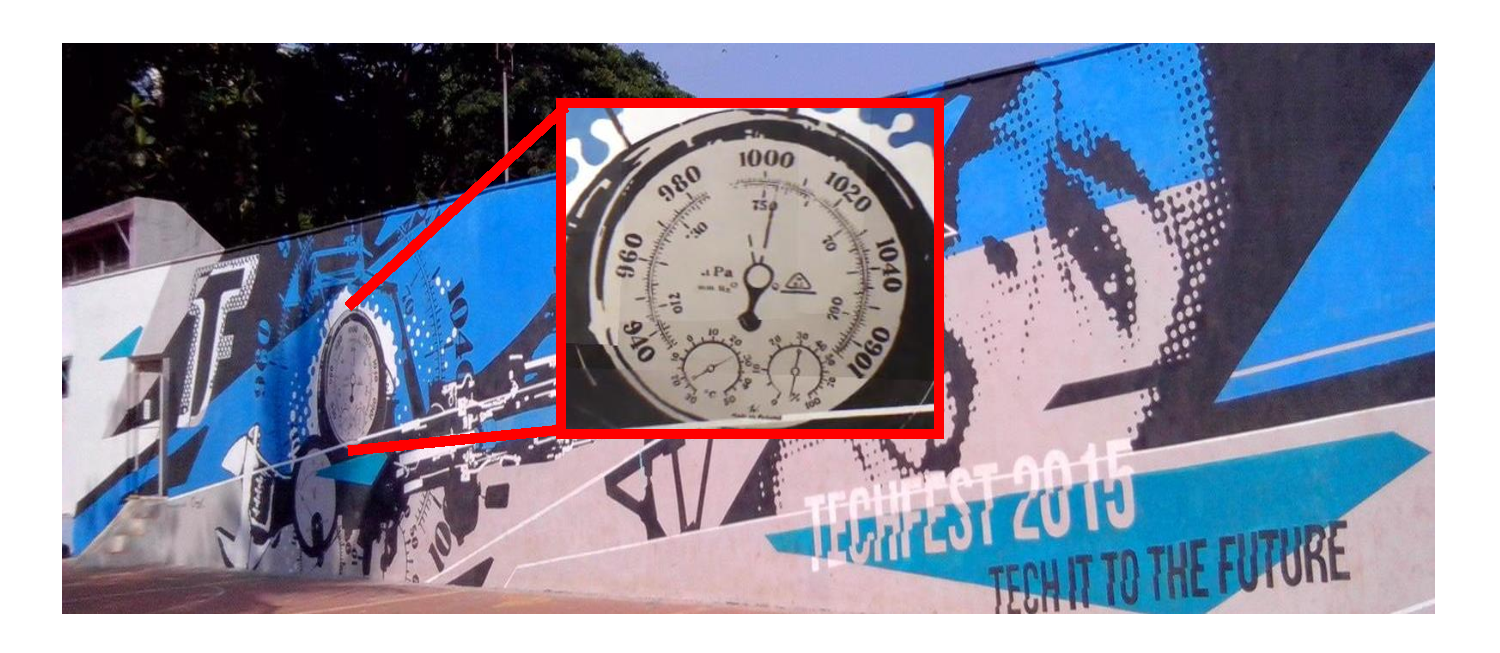
\includegraphics[width=0.98\linewidth]{figures/orthographicView}
\caption[Problems in imaging a large scene using a handheld
  camera]{Illustration of problems in imaging large planar scene with
  a handheld camera. A 40 feet wall captured with a handheld camera
  from a distance doesn't reveal details of the dial shown in the
  box. We wish to image such large planar structures by placing the
  camera close to and normal to the plane and later mosaic individual
  pieces.}
\label{fig:orthographicView}
\end{figure}

\emph{Quadcopters} (quadrotor helicopters) can be used to image large
planar surfaces from a close distance such as dams. Note that, as
mentioned above, we cannot capture an orthographic view of the entire
large planar surface from such distance in a single frame. In fact, we
will get a battery of images to encompass the whole scene
orthographically. These images must be stitched to get a panoramic
view.  Such a view will allow us to do post-processing as desired.

Panoramic construction requires alignment of overlapped
images~\cite{Brown03}.  These methods rely significantly on finding
common \textit{features} in overlapped images so as to establish
appropriate warps to register or align the images together. When we
attempt to use these methods for the purposes mentioned here, we noted
that there are cases where the imaged surface contains large textureless
regions. We term these regions as \emph{vacant spaces}. For example, in an art
gallery example shown in Figure~\ref{fig:indoor}, we have exhibits separated by
``empty spaces''. Notice that in Figure~\ref{fig:indoor}, images $\alpha$,
$\alpha'$, $\beta$, and $\beta'$ have `features', while images A, B, and C do
not have any significant features.  We can align images $\alpha$ with $\alpha
'$ as well as $\beta$ with $\beta '$, but not $\alpha$ with A, or C with
$\beta$.  Similarly, we cannot align A with B or B with C. Large homogeneous
vacant spaces result in scene regions that have little or no matches between
many significant images. As a result, we cannot create a panorama using
traditional mosaicing methods. In our example, we cannot build a bridge between
$\alpha$ and $\beta$ due to the presence of vacant space, which results in
disconnected components. Hence, there is a requirement of a method that can
infer positions to assist in mosaicing.  In this thesis, we propose the use of
quadcopters.

\begin{figure}[h!]
\centering
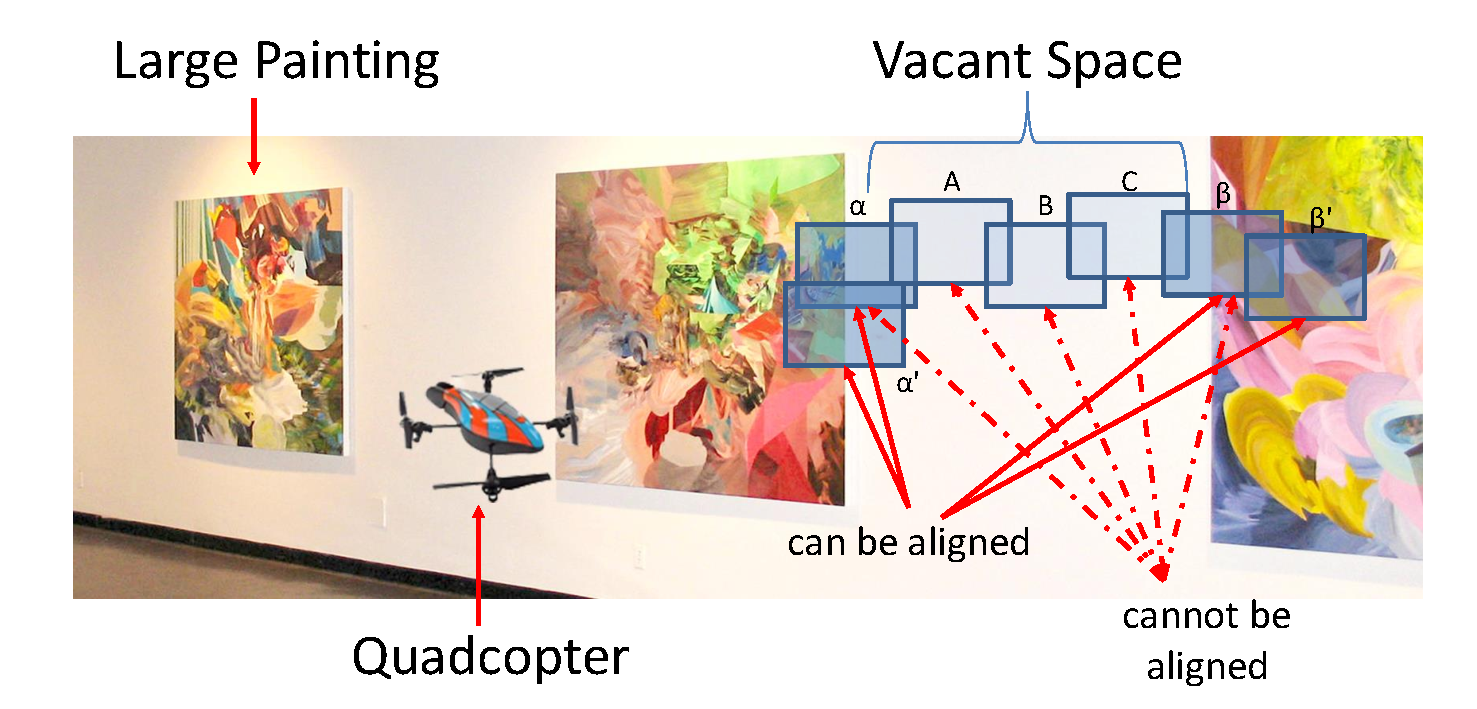
\includegraphics[width=0.98\linewidth]{figures/vacantSpaces/indoor}
\caption[Vacant spaces problem in art gallery]{Vacant spaces are
  encountered in the imaging of this scene. When individual portions
  are captured by a quadcopter, how does one create the complete
  mosaic, given that common features are unavailable? In this example,
  $\alpha$ and $\alpha '$ can be aligned, and so can $\beta$ and
  $\beta '$. This is not true for the constituents of the 5-tuple ($\alpha$, A,
  B, C, and $\beta$).}
\label{fig:indoor}
\end{figure}
    
Now, consider yet another situation where, with quadcopters as the
instrument, we would like to capture the paintings or murals on large
walls of a temple. We would like to ensure that details of the
painting are captured in a sufficient high definition. Often, temple
paintings are arranged in sequential order, depicting a particular
mythological story. In such cases, we would like to capture these
paintings spread over multiple walls and create an \emph{unrolled}
view of the scene where we get the output mosaic of the input scene as if it is
present on a single plane.  We have to make sure that capturing is done in a
manner such that full scene is imaged in minimum time to reduce inconvenience.

In such cases, we have to navigate the quadcopter smoothly to image
large multiplanar surfaces from a close distance. We examine current
options available for the navigation and control of quadcopter.  Most
predominantly, First Person View (FPV) controllers are available with
current quadcopters. However, considerable manual adjustments are
needed using the FPV to ensure specific depth, impacting the time of
capture. Next, if we have to capture large surfaces, the manual effort
is non-trivial.  Finally, as always with a manual procedure (and from
our experience), there is a high probability of collision during
these adjustments which may cause damage to the precious monuments.

The need for more control has led to software applications, typically
mobile based, for semi-autonomous navigation of a quadcopter.  As an
example, we can use these mobile applications to do basic maneuvers
(e.g., ``go from position X to position Y''). While these applications
are satisfactory for casual situations such as taking selfies, they
are unsuitable for the problem at hand.  For example, we cannot ensure
an orthographic view from a specific depth, even while traveling
autonomously along two dimensions of a large planar structure.  These
applications are not sufficiently autonomous either, to navigate the
quadcopter autonomously. Hence, there is a requirement of developing a
stable technique for autonomous navigation and control of quadcopters
in indoor as well as outdoor scenarios.
 
Imaging large multiplanar surfaces using a single quadcopter in one
flight is not always feasible due to battery constraints. In such
cases, one may use multiple quadcopters in collaboration. The
identification of every quadcopter under motion is essential for using
multiple quadcopters. Fiducial markers such as ARTag have been used to
identify objects. However, due to the swift motion of a quadcopter, a
significant amount of motion blur is introduced. If such fiducials are
placed on non-stationery objects, they do not get recognized because
recognition of these fiducials depends on the detection of geometric
patterns such as lines, corners, etc.  Hence, there is a necessity of
developing blur resilient fiducials which can be recognized robustly
when placed on swift moving objects such as quadcopters.

\section*{Problem Statement}
\textit{The problem of autonomous navigation of quadcopters to image
  multiplanar surfaces containing vacant spaces with correct
  identification of individual quadcopter forms the problem statement
  of the work presented in this thesis.}

We decompose our problem of mosaicing a multiplanar scene containing
vacant spaces through the autonomous navigation of one or more
quadcopters into the following steps:
\begin{enumerate}
  \item Mosaicing a \textit{single} planar scene, possibly containing vacant
  spaces.
  \item Autonomous navigation of quadcopter for imaging a multiplanar scene.
	\begin{enumerate}
  		\item Path planning for imaging each planar region in a multiplanar scene.
	\end{enumerate}
  \item Unrolling scenes spread over multiple planes.
  \item Devising a mechanism for robust recognition of quadcopters under swift
  motion.
\end{enumerate}
Each of these steps is non-trivial and challenging as explained in
next section. In this thesis, we deal with these steps by leveraging
the additional information available onboard the quadcopter.

In considering quadcopters, we briefly consider factors for the selection of
the imaging instrument. We require at a minimum three characteristics in
quadcopters to achieve the goal of autonomous navigation. First, quadcopters
should have a camera with reasonable resolution (at least 1080 x 720
pixels). Second, they should be able to communicate with a computer
through a well-established protocol. Third, we should be able to fly
them indoors as well as outdoors. The cost is clearly a factor once
these three requirements are satisfied.

The first requirement is met in most of the quadcopters, but only a
few quadcopters satisfy the second and third requirements
simultaneously. For example, the DJI Phantom 4, costing around 1200
USD has a camera mounted on 3-axis gimbal coupled with a gyroscope. It
enables us to take very stable videos while flying. There are FPV
controllers as well as mobile applications available for
semi-autonomous navigation of DJI Phantom 4. But as discussed earlier,
these options are not useful in solving our problem.  Also, there is
inadequate open-source software support for autonomous navigation of
DJI Phantom 4.

Some quadcopters have a GPS to assist navigation. But we cannot use
GPS facility in an indoor scenario. Even if the GPS signal is
available, we cannot rely only on GPS for navigation of quadcopters in
outdoor scenarios due to GPS jamming and the spurious GPS signals.

Octocopters such as DJI S1000 have excellent flight control as well as
stability. But due to their bulky nature (weight around 11Kg), we
cannot use it in indoor areas. There are a few non-commercial
quadcopter systems which have gained focus, e.g., the team at the
University of Pennsylvania has developed a series of quadcopters
capable of doing unbelievable maneuvers. However, such systems use
high-speed motion camera systems such as Vicon to find out the pose of
the quadcopter in motion. Hence, we cannot use them in uncontrolled
environments.

Parrot's ARDrone and Bebop are two reasonably priced (USD 350 and USD
700 respectively) quadcopters having HD camera with resolution 1280 x 720
pixels. Though they are lightweight (0.42 kg) compared to the DJI Phantom 4
(around 1.4kg), they are robust enough to withstand outdoor conditions. ARDrone
streams a WiFi hotspot to which any computer can be connected. Parrot has also
released an SDK which is essential to do interfacing with these quadcopters.
When I had started work on quadcopters (in mid-2013), Parrot's Bebop was not
available. Hence, I have used Parrot's ARDrone 2.0 for my research work
presented in this thesis.

\section*{Challenges}
\label{sec:challenges}
The challenges which make our problem interesting to solve are as follows.

\begin{itemize}
  
\begin{figure}[h!]
\centering
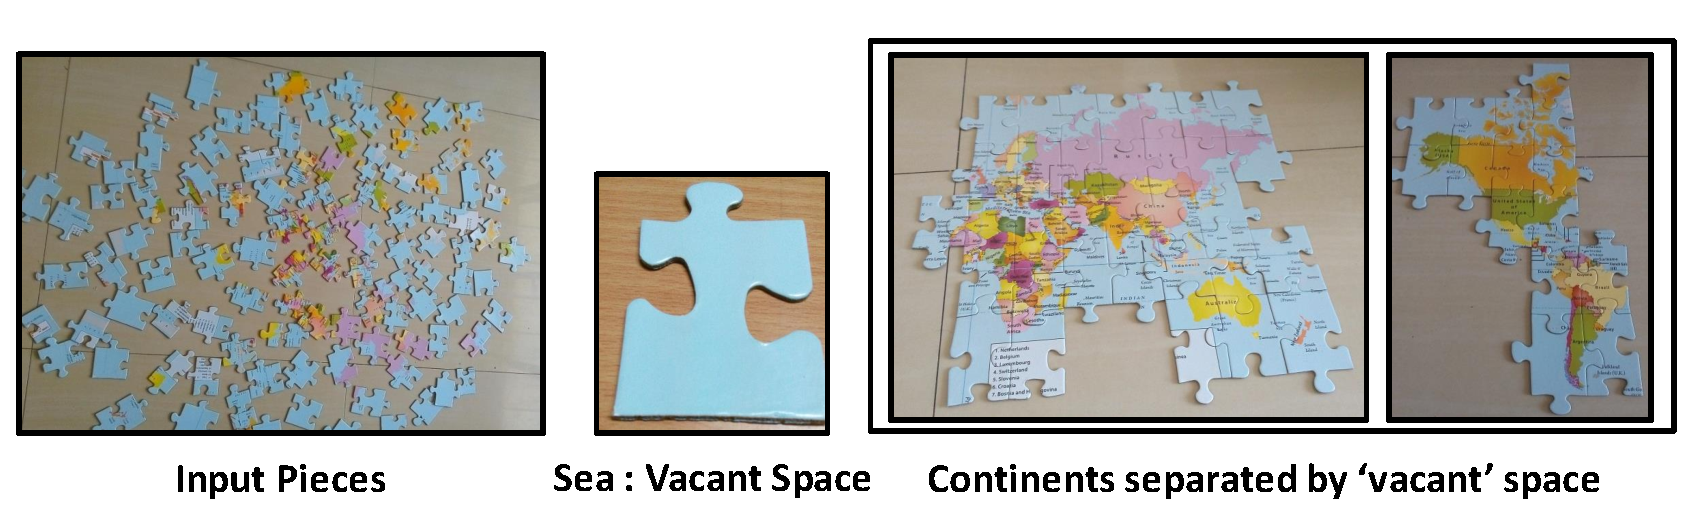
\includegraphics[width=0.98\linewidth]{figures/vacantSpaces}
\caption[Jigsaw Puzzle as a mosaicing problem]{Jigsaw Puzzle as a mosaicing
problem. Individual pieces (Left) of a jigsaw puzzle can be thought of constituent images of mosaic. Due to featureless
regions belonging to the ocean (shown in Middle), one may find it difficult to join
``Americas'' with remaining continents as shown in (Right). We have to use
our knowledge about geography to complete the puzzle.}
\label{fig:vacantSpaces}
\end{figure}
  
  \item \textbf{Vacant spaces and regions with confusing features:}
    Mosaicing a scene is similar to solving a jigsaw puzzle like the one shown in
  Figure~\ref{fig:vacantSpaces}. Here, individual pieces of the puzzle can be
  thought of as constituent images in a mosaic. We have to match
  pieces and join them. This is similar to the stitching algorithms
  which find matches in two images for estimating the relative position of one
  image with respect to another image. Normally, pieces can be placed at their
  correct positions by matching a color, texture, as wells as a shape on the piece,
  e.g., if there is a red colored piece, we can consider only other red
  colored pieces whose boundaries match with the first piece. The blank
  pieces representing the seas make such puzzles hard to solve. While solving
  jigsaw puzzle containing blank pieces, we could build the parts of the
  puzzle, e.g., ``Americas" and rest of the world as shown in
  Figure~\ref{fig:vacantSpaces}. However, we cannot place these parts at
  their respective positions as we cannot match these parts with blank
  pieces to complete the puzzle. Here, we have to use additional positional
  information (e.g., geography in the puzzle shown in
  Figure~\ref{fig:vacantSpaces}) to join different parts separated by
  vacant spaces. In general, images containing very less or no features are
  difficult to match.

  The standard mosaicing method uses feature matching algorithms for
  estimating the homography between two images. Feature matching algorithms
  require detection of sufficient features in both images. However, scenes like
  Figure~\ref{fig:vacantSpacesExample}(left) contain large regions with vacant
  spaces. Such regions result in very few (or almost zero) features which pose
  a problem for stitching images containing such regions. The output (shown in
  Figure~\ref{fig:vacantSpacesExample}-right) of Adobe Photoshop~\cite{photoshop}, 
  a popular mosaicing software showcases the inability to handle vacant spaces.
  
 \begin{figure}[h!]
\centering
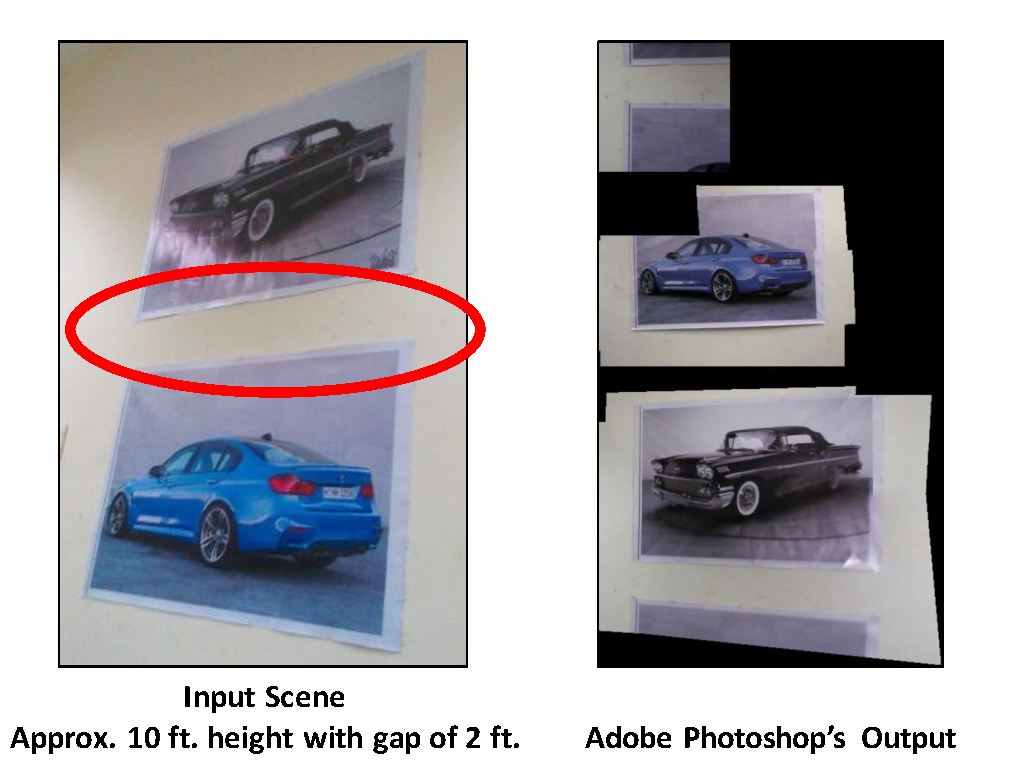
\includegraphics[width=0.98\linewidth]{figures/vacantSpacesExample}
 \caption[Problem of mosaicing scene with vacant spaces using Adobe
 Photoshop]{Is Mosaicing problem solved? Standard stitchers such as Adobe
 Photoshop~\cite{photoshop} cannot stitch images which have none or very little
 features in common. Left: there is an input scene containing vacant space
 separating the two posters (indicated by the red oval). Right: Adobe Photoshop
 outputs individual pieces instead of complete mosaic as feature matching
 algorithm fails.}
\label{fig:vacantSpacesExample}
\end{figure}
 
  There is another problem with standard stitching algorithms due to 
  reliance on feature matching. The feature matching algorithm gets confused
  when parts of the scene are repeated. It results in images which are not
  taken from adjacent positions being stitched together.
  Figure~\ref{fig:confusingFeatures} shows output of
  AutoStitch~\cite{autostitch}, the state of the art stitcher, on an input scene
  containing repetitive patterns. It can be seen that images taken from
  positions far apart from each other get stitched together as the matching
  algorithm matches features from those images.

\begin{figure}[h!]
\centering
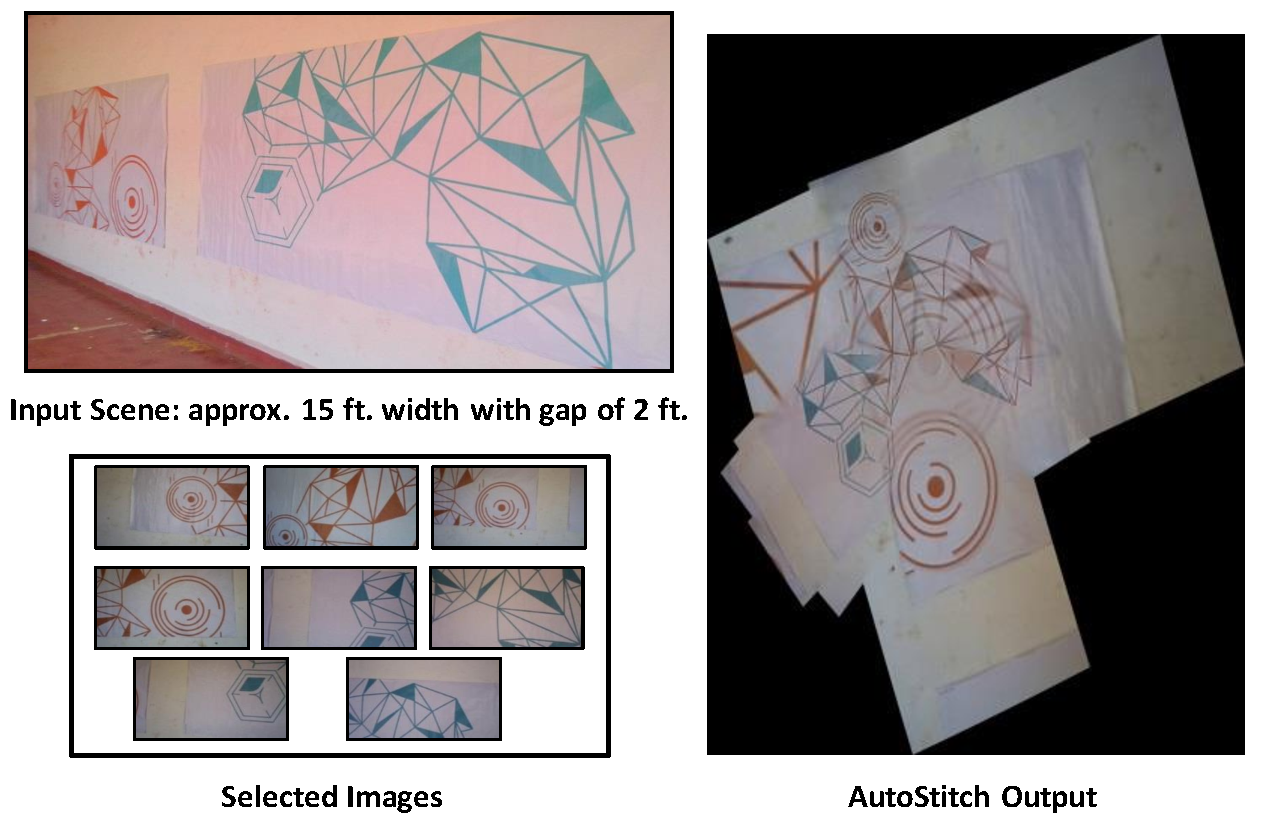
\includegraphics[width=0.98\linewidth]{figures/confusingFeaturesExample}
\caption[Problem of confusing features in AutoStitch]{Repetitive patterns in the
input scene pose a challenge for standard mosaicing methods such as
AutoStitch~\cite{autostitch}. Images taken from positions far apart from each
other get stitched together as matching algorithm matches features from those
images.}
\label{fig:confusingFeatures}
\end{figure}  

  \item \textbf{Control and navigation of an inexpensive quadcopter:}
  Inexpensive quadcopters like Parrot's ARDrone are agile and can do
  several maneuvers swiftly. However, manually controlling a quadcopter to image large
  planar regions smoothly by keeping a constant distance from the imaging plane
  is very difficult because of the tendency of quadcopter to drift from its
  desired position. Hence, there is a requirement of a mechanism for autonomous navigation of
  quadcopter. One does not have to image the scene continuously while navigating
  the quadcopter as too many pictures are redundant. We have to estimate the
  optimal number of positions of the quadcopter from where it can take images,
  even while ensuring that captured images encompass the scene.
  
  \item \textbf{Building a scale accurate 3D map of the environment in
  real-time:} A quadcopter has to be maneuvered along an estimated path such
  that it will cover the input scene in minimum time. We require accurate
  3D coordinates of the region to be imaged on the fly for doing efficient path
  planning. Researchers generally use RGBD cameras such as the Microsoft
  Kinect~\cite{Zhang:2012} for getting a 3D map of the environment. However,
  due to payload restrictions as well as battery requirements, it is not
  efficient to put such cameras on top of a quadcopter like ARDrone. Structure
  from Motion (SfM) techniques can build such a 3D map, but due to the
  real-time requirement, we cannot use such techniques. There are various
  methods based on popular techniques such as Simultaneous Localization and
  Mapping (SLAM) or Parallel Tracking and Mapping (PTAM) for creating a 3D map
  of the environment. However, most of these methods, e.g.,~\cite{klein}, lack
  the accuracy in scale estimation due to complete reliance on visual feedback,
  resulting in an erroneous 3D map. Engel et al.~\cite{engel} have developed a
  method which fuses IMU measurements with the PTAM measurements, to create a
  3D map for camera-based navigation of a quadcopter. However, it is not
  sufficiently precise for our purposes due to inaccuracies in scale.
  
  \item \textbf{Robust detection of multiplanar bounded regions in real-time:} 
  Multiplanar imaging through quadcopter requires detection of multiplanar
  bounded regions in real-time. There are a few methods like
  multiRANSAC~\cite{zuliani}, J-linkage~\cite{jlinkage},
  T-linkage~\cite{tlinkage} in the literature for detection of multiple planes
  from the input data. These methods do not output the boundaries of planar
  regions. They only output the estimated planes from the input 3D points using
  geometric affinity of points towards individual planes. Also, these methods
  have not considered the validity of boundaries of planar regions to remove
  noisy points. As a result, such noisy points get clustered into wrong planes,
  extending boundaries of planar regions incorrectly.
  Figure~\ref{fig:jlinkageProblem} illustrates this problem. Points marked by
  black oval are the result of erroneous estimations by PTAM, i.e., marked
  points labeled as plane B actually belong to the plane A and vice-versa. 
  Since their geometric affinity is towards opposite planes, they are labeled
  incorrectly.

\begin{figure}[h!]
\centering
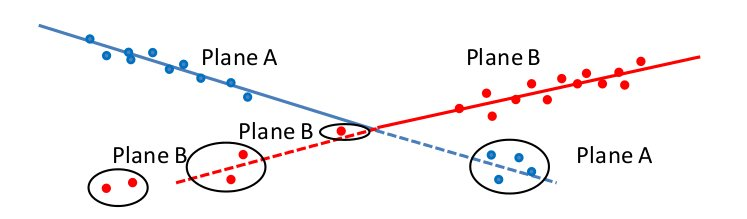
\includegraphics[width=0.98\linewidth]{figures/multiplanar/JlinkageProblem}
\caption{Problem in J-linkage clustering. J-linkage doesn't use validity of plane
boundaries to cluster points to correct planes. Points marked by black ovals
are the result of erroneous estimations by PTAM. Since their geometric
affinity is towards opposite planes, they are labeled incorrectly.}
\label{fig:jlinkageProblem}
\end{figure}

  \item \textbf{Identification of a quadcopter under motion:}
  Imaging large multiplanar scenes using a single quadcopter is difficult 
  due to the insufficient power available in the battery. Multiple 
  quadcopters can be used in such scenarios to work in collaboration. Each
  quadcopter requires to be distinguished. The movement of quadcopter like
  ARDrone is quite jerky which results in motion blur in images of quadcopters.
  It makes tracking of such quadcopters challenging. Normally, we can place
  fiducials on the quadcopter to keep track. ARTag~\cite{Fiala05} is preferred
  over other fiducials like ARToolkit~\cite{ARToolkit02}, PiTag~\cite{Pitag13},
  etc. as the recognition rate of ARTag is better than other existing fiducials.
  However, none of these fiducials are recognized in the presence of motion
  blur. Figure \ref{fig:ARTagBlur} demonstrates the problem in recognition of
  ARTag under motion blur. Figure \ref{fig:ARTagBlur} (Left) shows that ARTags
  get recognized (indicated by green rectangles) in the absence of blur in
  captured images. However, when there is a significant amount of blur, ARTags cannot be
  recognized (Figure \ref{fig:ARTagBlur} (Right)).
  
\begin{figure}[h!]
\centering
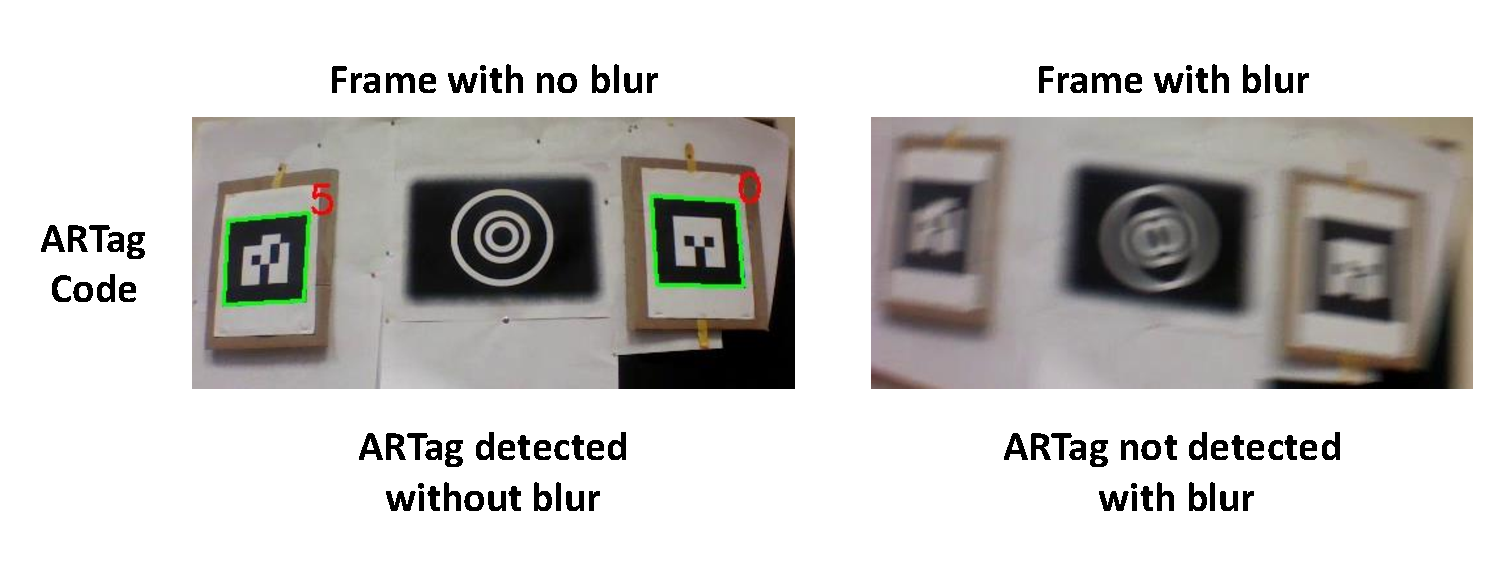
\includegraphics[width=0.98\linewidth]{figures/fiducial/ARTagBlur}
\caption[Problem of motion blur in ARTag]{Illustration of problem with ARTag.
There are two ARTags in the scene.
When there is no blur in the captured image (Left), both ARTags are recognized
(indicated by green rectangle). When there is motion blur in the captured
image (Right), neither of the two tags are recognized.}
\label{fig:ARTagBlur}
\end{figure}

\end{itemize}

\section{Contributions of this thesis}
\begin{figure}[h!]
\centering
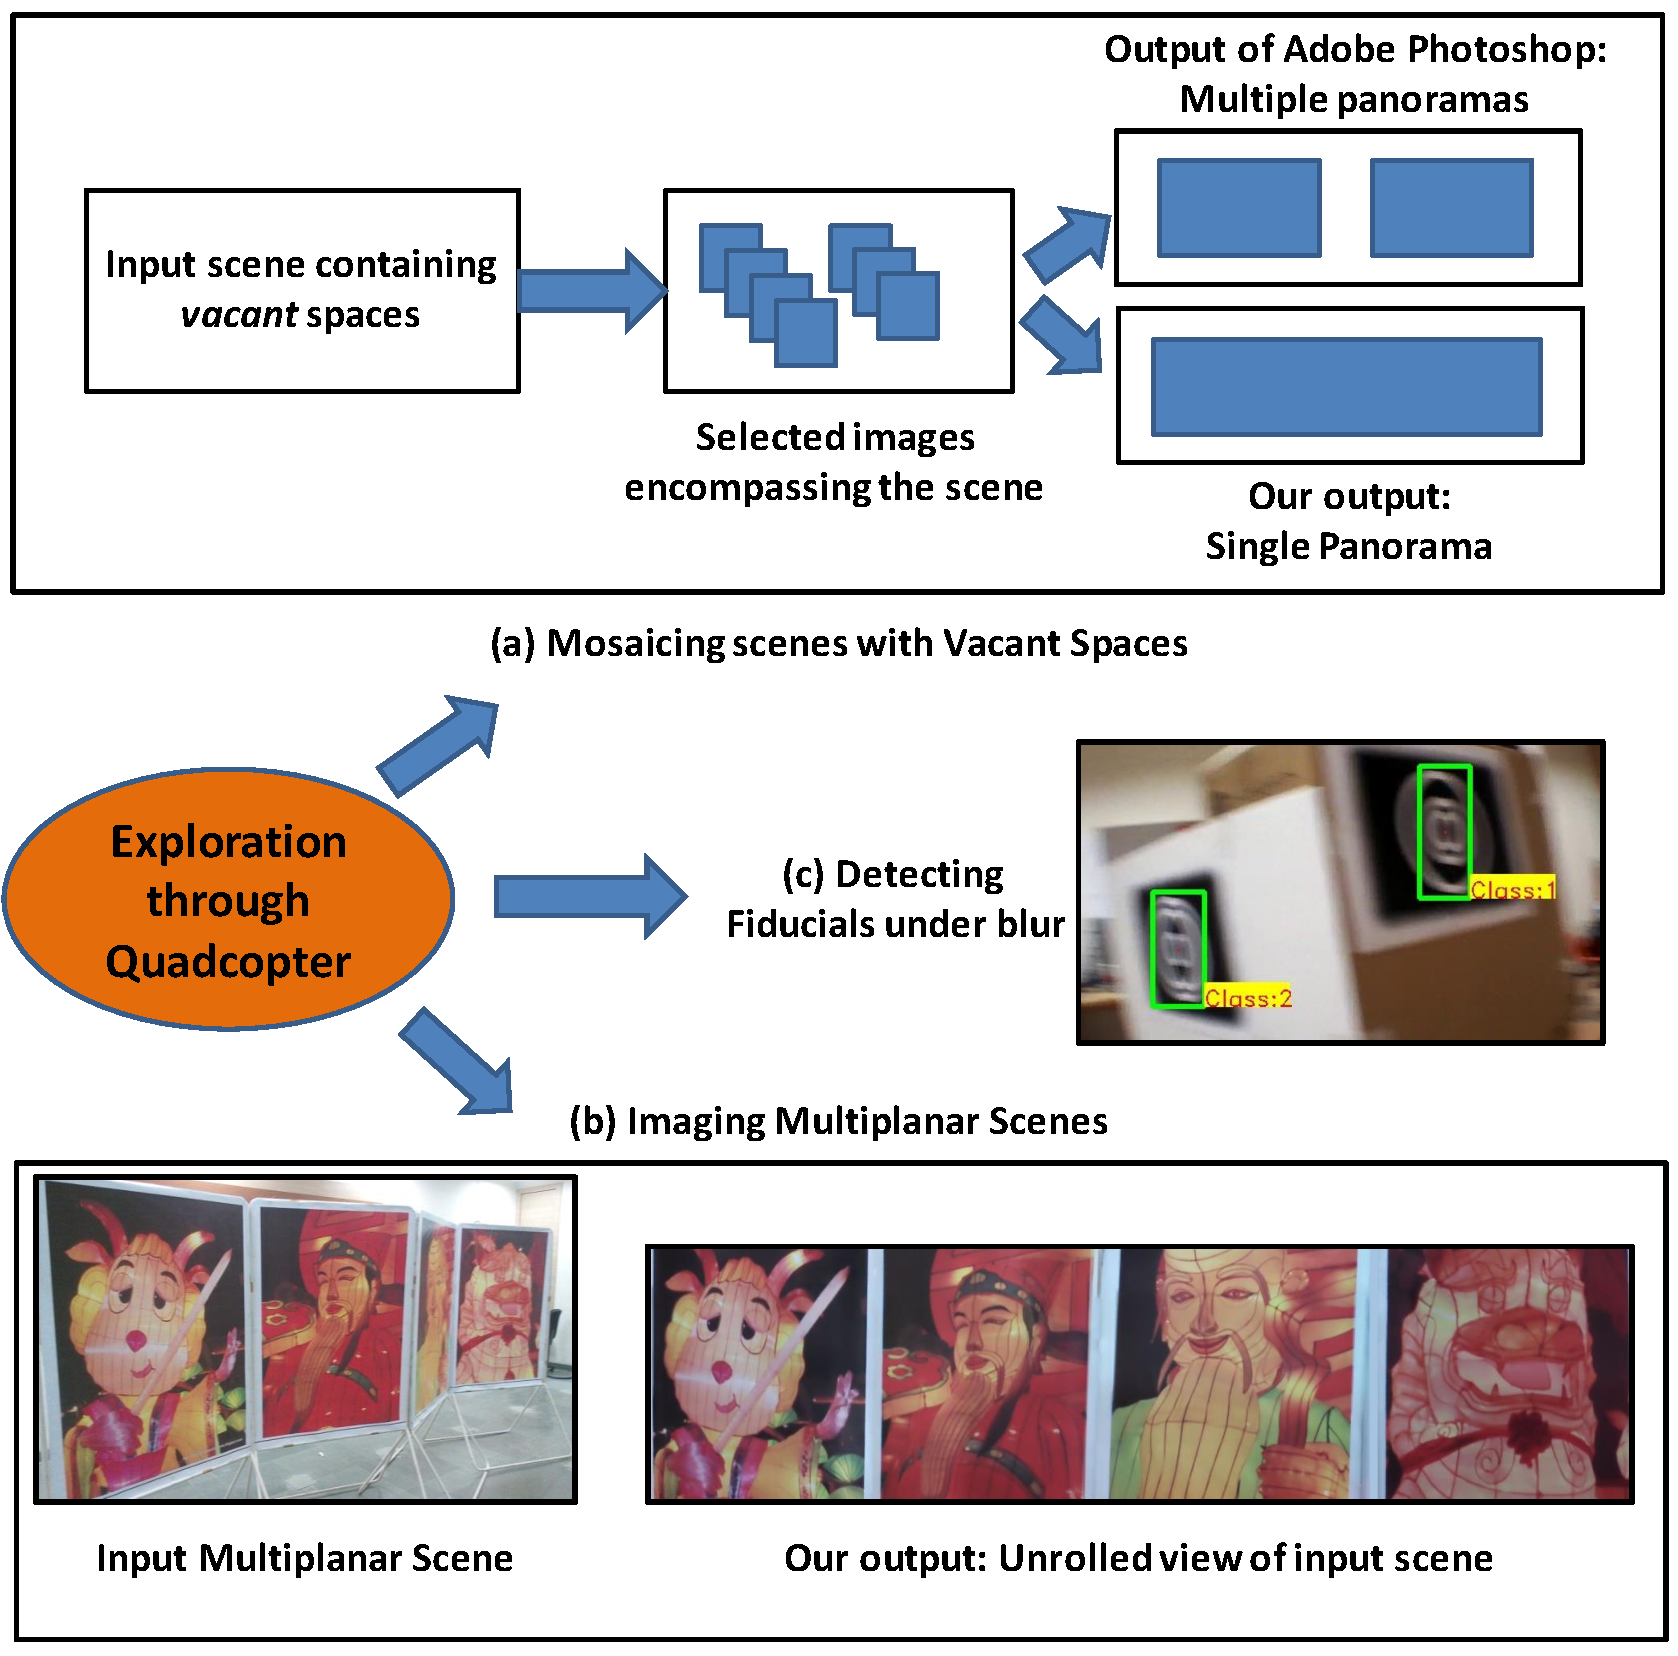
\includegraphics[width=0.98\linewidth]{figures/contributions2}
\caption[Contributions]{Our work involves techniques required for imaging
multiplanar surfaces through one or more quadcopters. (a) Shows mosaicing of a scene containing
vacant spaces. Two exhibits on a wall are separated by  a large vacant space
which makes homography based stitching methods ineffective. (b) Shows imaging
of a multiplanar scene through quadcopter. We imaged a multiplanar scene in such
a way that content on each plane is imaged with an orthographic view. Later we
combined a mosaic from each planar bounded region to get the  unrolled view of
an overall scene. (c) Shows our blur-resilient fiducials being recognized in the
presence of motion blur, even from oblique angles.}
\label{fig:contributions}
\end{figure}

As shown in Figure \ref{fig:contributions}, we have developed an integrated solution to
explore scenes spread over single or multiplanar scenes through quadcopter. To
the best of our knowledge, we are the first to use quadcopter for:
\begin{itemize}
  \item Mosaicing scenes with vacant spaces  
  \item Imaging scenes spread over multiple planes autonomously   
\end{itemize}

Specific contributions made to achieve this goal and to address the above
mentioned challenges are:\\

\subsection{Mosaicing Scenes with Vacant Spaces}
\begin{figure}[h!]
	\centering
	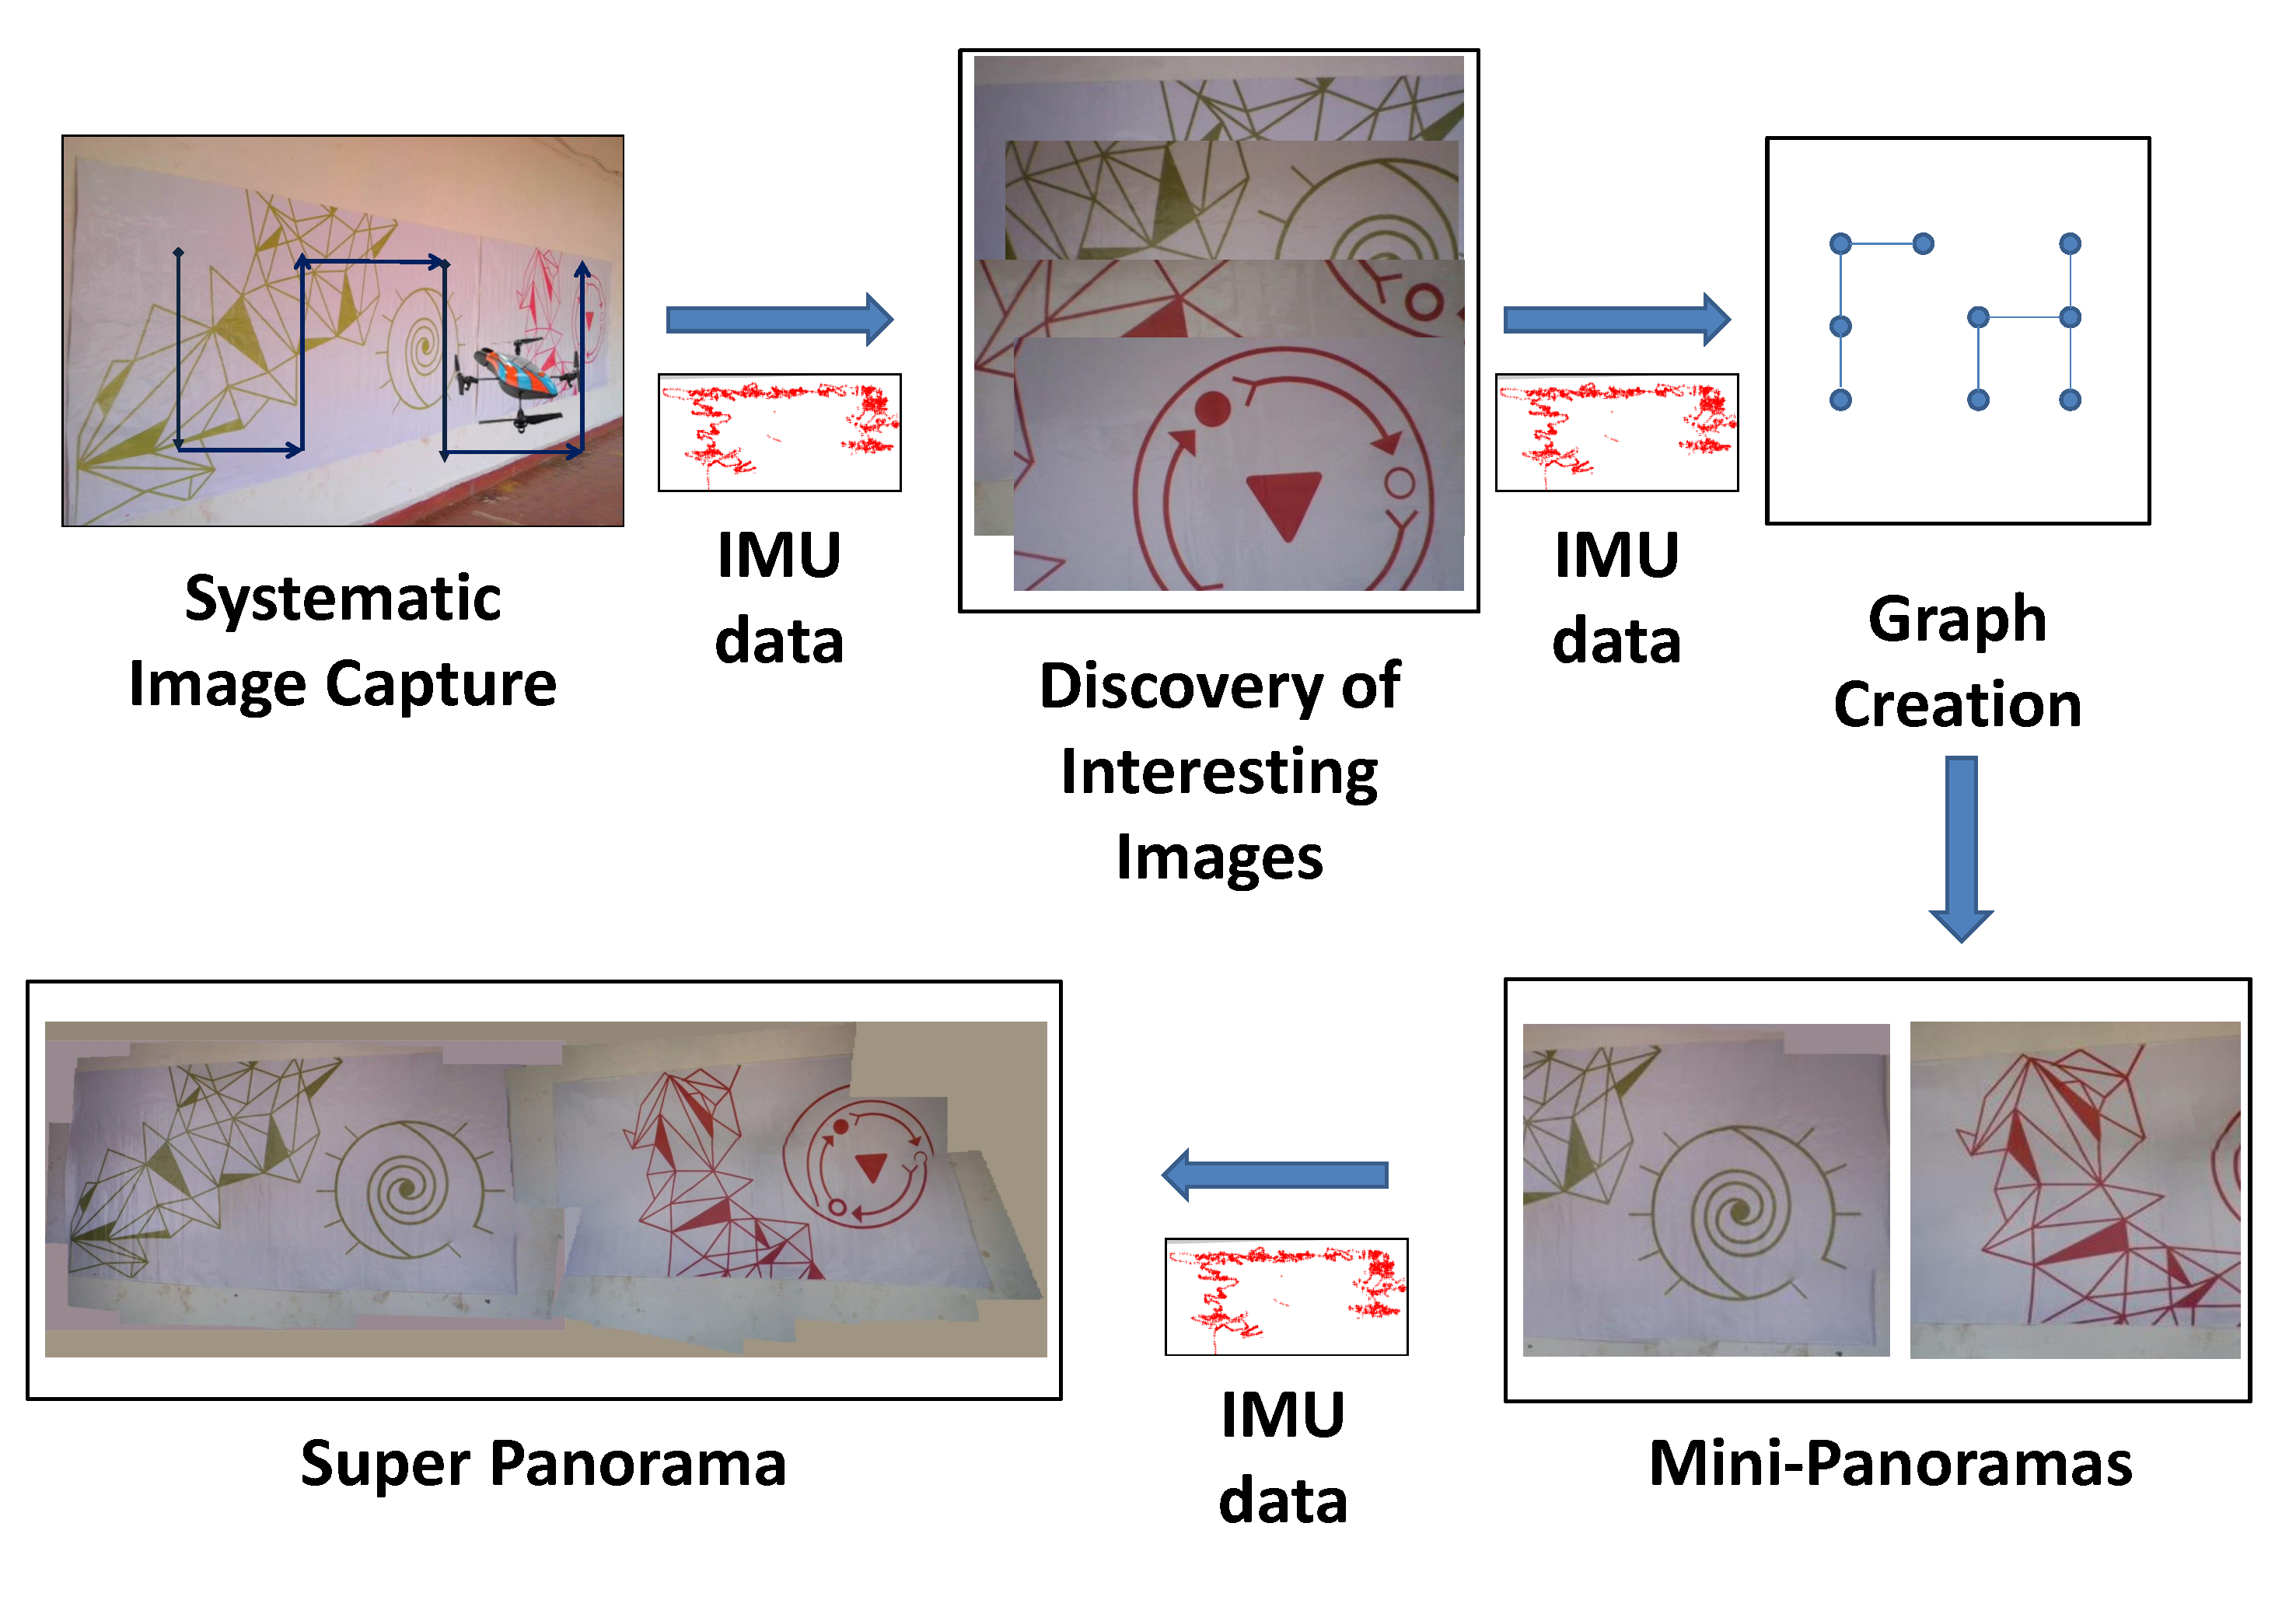
\includegraphics[width=0.98\linewidth]{figures/vacantSpaces/Workflow}
	\caption[Workflow]{ Overview of mosaicing scenes with vacant spaces: Input
	imagery is systematically acquired (top left) by a quadcopter.  In the next
    step, interesting images are found by clustering the video into
    regions based on positional data.  A graph is constructed using
    proximal images. For each connected component in a graph, standard
    stitching techniques are used to create mini-panoramas which are
    then joined together into a super panorama 
    again using IMU data.}
    \label{fig:vaccantSpaces_workflow} 
  \end{figure}
  
  We propose to solve the vacant space problem by using additional information
  available from an inexpensive quadcopter. Quadcopter contains an inertial
measurement unit (IMU) that has positional information. We use the positional
information from IMU primarily for two purposes:
\begin{enumerate}
\item \textbf{Selection and ordering of images:}
We use the IMU data to select representative images from the video and arrange
them into rectangular grid according to the `spatial' neighborhood. It also
  disambiguates situations when multiple images that are spatially distant,
  have similar, repeated features.

\item \textbf{Super-panorama:} Whenever there are no features in
  the overlap region of two images, we use the IMU data to find the
  relative position of one mini-panorama with respect to another.
\end{enumerate}

However, IMU data on a quadcopter cannot be relied exclusively, or sometimes at
all, especially on inexpensive devices. Our experiments indicate that roll
and pitch angles (depending on the distances involved) may be completely off,
and so can the physical coordinates.  This is a consequence of jerky,
swift movements.  Complementing the IMU with information gleaned from
vision algorithms, however, may be a useful practice.

The method adopted is pictorially depicted in the overview shown in
Figure~\ref{fig:vaccantSpaces_workflow}.  In brief, we systematically acquire a 
video of the scene, reduce the input video to a manageable number of images, and finally, 
combine the images acquired from different positions into a mosaic. 

The result on a sample scene is shown in Figure~\ref{fig:vacantSpaces_result}.
In this experiment, the input stream had about 9000 input images.  Our selection algorithm
 pruned the video into $N=13$ images. A sample of the selected images are seen
 in Figure~\ref{fig:vacantSpaces_result}(a).  The scene as captured by a
 smartphone can also be seen, as well as the outputs of the state of the art
 stitchers, viz., AutoStitch\cite{autostitch} and Adobe
 PhotoShop\cite{photoshop}. Note that AutoStitch\cite{autostitch} is only able
 to stitch the upper half of the scene.  Our result
 Figure~\ref{fig:vacantSpaces_result}(e) clearly stands out in comparison.\\
  
  \begin{figure}[h!]
	\centering
	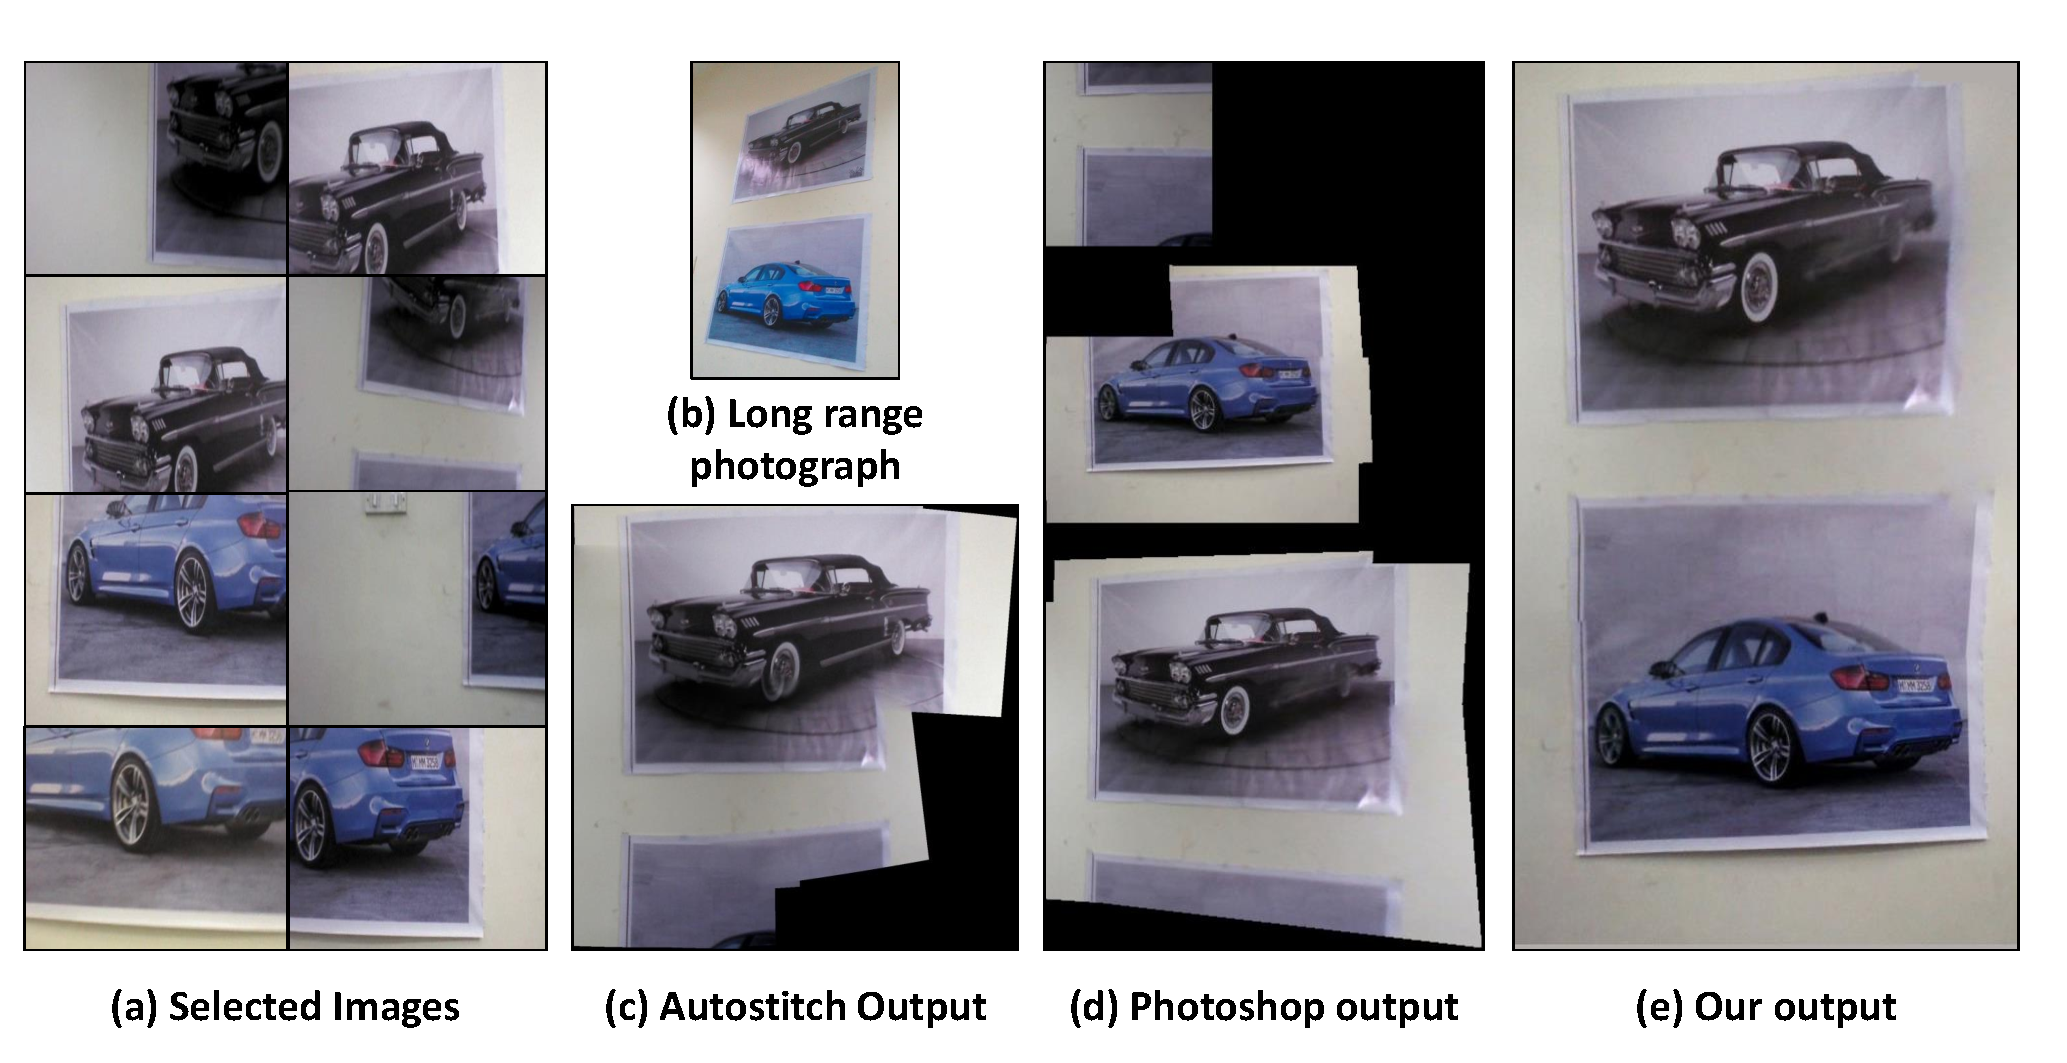
\includegraphics[width=0.98\linewidth]{figures/vacantSpaces/indoor_results}
	\caption[Result: Cars]{ (a) Pruned images from the quadcopter video using our
  saliency algorithm of (b) an indoor scene. This long range photograph
  has been captured separately by a smartphone camera only for the
  context. Notice a significant vacant space in the imagery.  (c)
  Output of AutoStitch -- only the upper half of the scene is output.
  (d) Output of Adobe Photoshop CS6 -- the vacant space posed a problem to the
  feature matching algorithm, so instead of a mosaic, individual
  pieces were output as mini-panoramas (e) Our output on the selected
  images. We are able to present the scene in high fidelity in an
  orthographic view.}	
	\label{fig:vacantSpaces_result}
	\end{figure}
  
\subsection{Autonomous Multiplanar Imaging through Quadcopter}
\begin{figure}[h!]
\centering
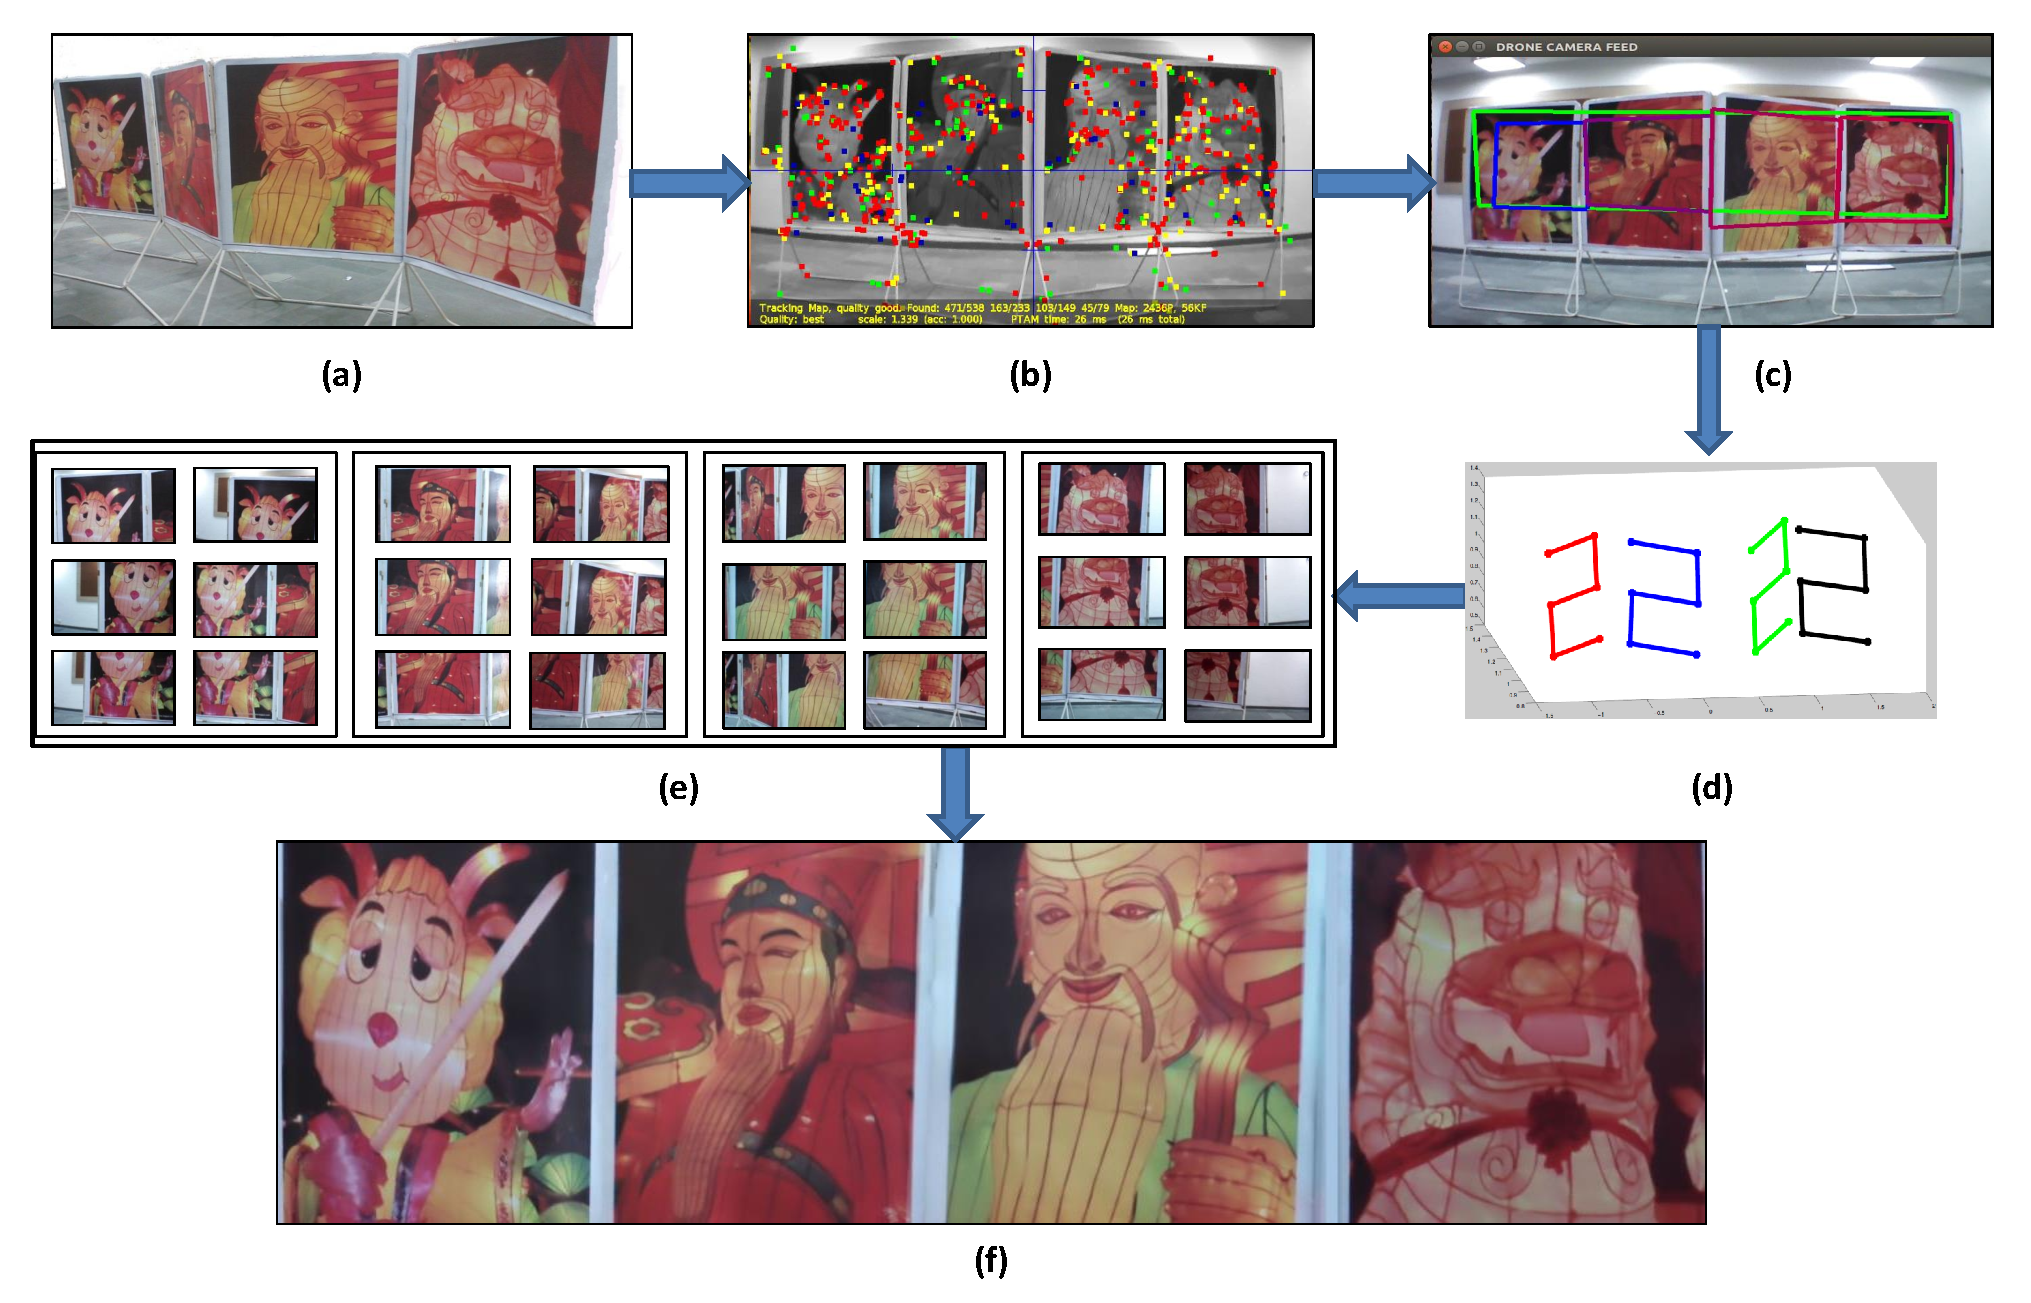
\includegraphics[width=0.98\linewidth]{figures/multiplanar/workflow}
\caption[Overflow of autonomous multiplanar imaging through quadcopter]{Overview
of Multiplanar Imaging through quadcopter:
(a) An input Scene to be imaged.
(b) Feature points in the scene are found and their 3D positions are estimated
using scale aware PTAM \cite{Engel12}. (c) Multiple planar bounded regions are
estimated using our algorithm. (d) For each bounded planar region, 3D camera
positions are calculated and overall path planning is done. (e) Videos are
captured at each target position. From each captured video, the appropriate
frame is found. (f) Individual mosaics are joined together to get final output.}
\label{fig:multiplanar_workflow}
\end{figure}

The mosaicing algorithms can mosaic only if the scene lies on a single planar
surface. But the real world is made of multiplanar as well as curved surfaces.
In fact, we have many circumstances where the input scene is spread over
multiple planes. In such cases, we would like to image each planar region
orthographically and then `unroll' the whole scene by joining the individual
mosaics so that we get the output mosaic of the input scene as if it is present
on a single plane.

The method adopted is pictorially depicted in the overview shown in
Figure~\ref{fig:multiplanar_workflow}. In brief, we probe the input scene through a quadcopter, calculate the 3D positions of feature points
using PTAM based method\cite{engel}. Later we use our algorithm, an improvement
over j-linkage\cite{jlinkage} to detect multiplanar bounded regions from the area
marked by the user through our user interface. Path planning is done for each
planar bounded region to find out the camera positions in such a way
that images captured from those positions encompass the scene in an optimal manner.
The quadcopter is autonomously maneuvered along the estimated path and videos
are captured at target points. For each planar bounded region, the appropriate
frame from each video is found and then given to a mosaicing algorithm. 
Finally, all mosaics are joined together to get a full unrolled view.

Our experiments are done on various setups covering multiple planes.
In one such experiment, paintings were arranged in the convex
fashion as shown in Figure~\ref{fig:multiplanar_result} (Top-Left). We have
selected the area to be imaged as shown in Figure \ref{fig:multiplanar_result}
(Top-Right). In the path planning stage, overall 30 (9 from the left plane, 12 from the middle
and 9 from the right plane) positions to cover full region are estimated.  Images
captured from those positions are mosaiced using our algorithm to get the final
mosaicing output as shown in the Figure~\ref{fig:multiplanar_result} (Bottom).
\begin{figure}[h!]
	\centering
	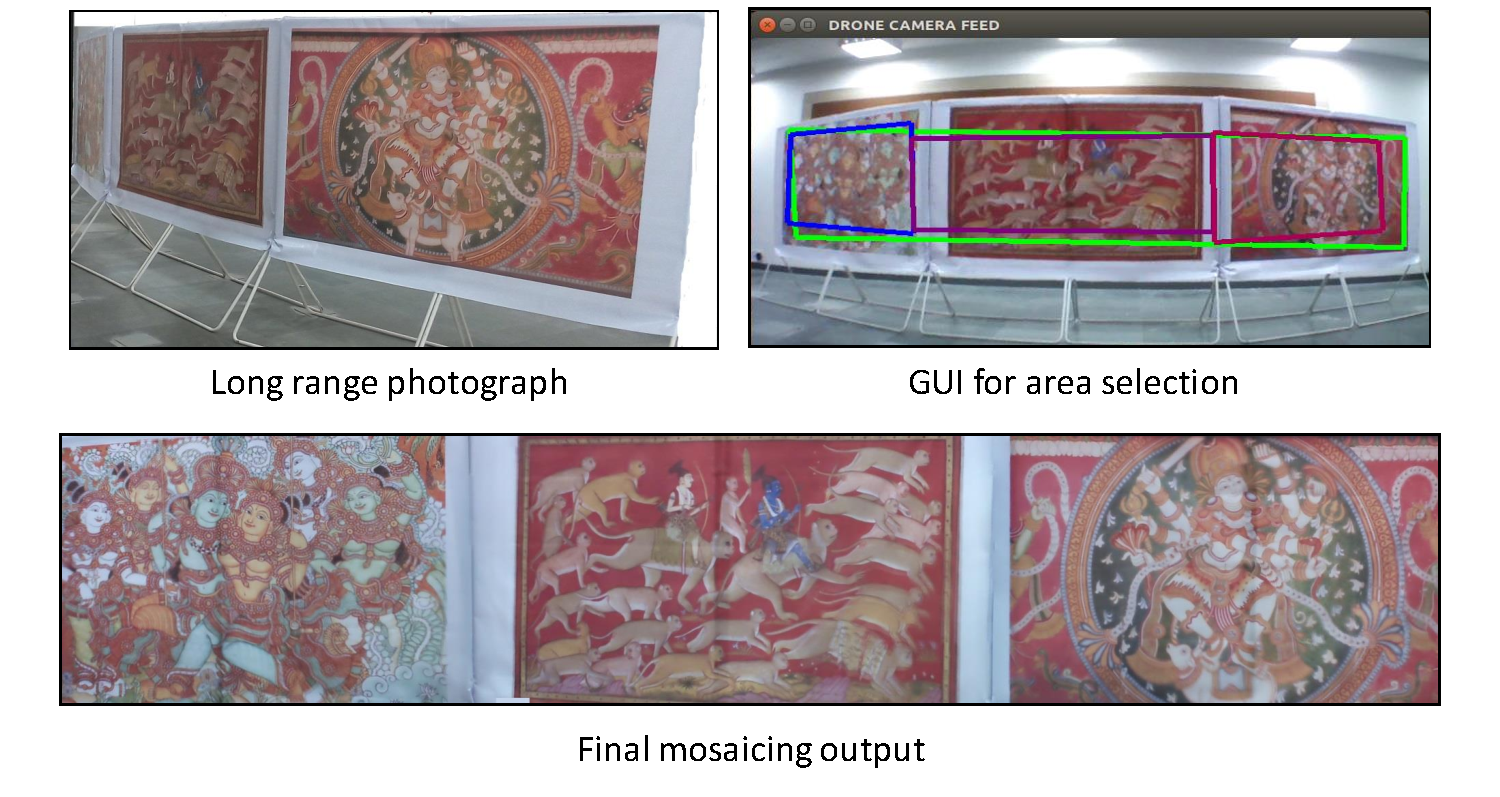
\includegraphics[width=0.98\linewidth]{figures/multiplanar/convexResult}
	\caption[Result: Imaging Convex Surface ]{The exhibition of 
	temple paintings arranged in convex fashion as shown in the long range photograph (top-left). Note that we
cannot cover all paintings with enough details simultaneously. We have selected
the area to be imaged as shown in GUI for area selection (top-right).
Green quadrilateral shows the user selected area while blue, violet and magenta
colored quadrilaterals represent the multiple planar bounded regions
estimated by our algorithm. In the path planning stage, overall 30 (9 from left
plane, 12 from middle and 9 from the right plane) positions were estimated to cover
the full region. Images captured from the estimated positions are mosaiced using
our algorithm to get the final mosaicing output as shown in the bottom image.}	
	\label{fig:multiplanar_result}
\end{figure}
	
\subsection{Blur Resilient Fiducials for Quadcopter}

\begin{figure}[h!]
\centering
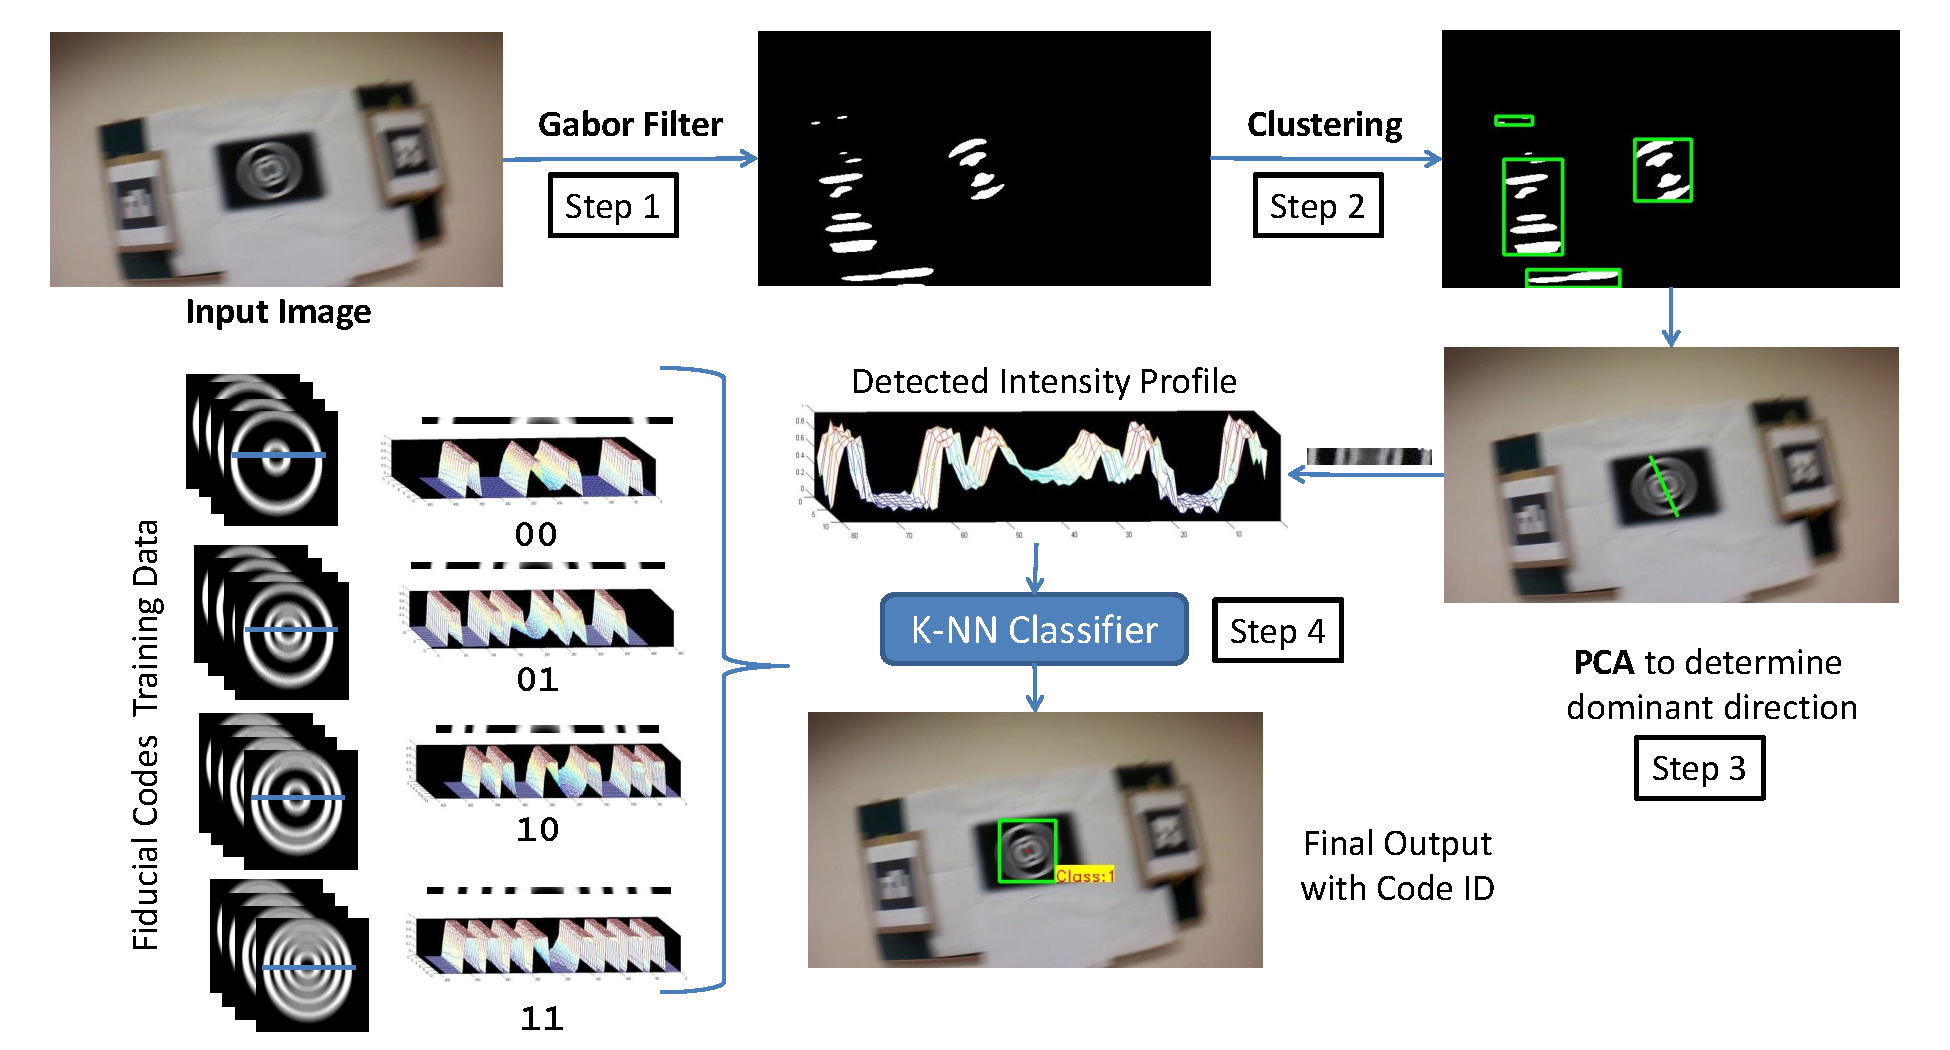
\includegraphics[width=0.98\linewidth]{figures/fiducial/overall_flow}
\caption[Overall Workflow of blur resilient fiducial recognition algorithm]{An
overview of our fiducial recognition algorithm.
    The four step process includes (Step 1) Filtering,
    (Step 2) Component clustering, (Step 3) Dominant direction determination
    and (Step 4) Classification using prior training data.}
 \label{fig:fiducial_workflow}
\end{figure}

A single quadcopter is not sufficient for imaging large multiplanar scenes due
to battery constraints. Instead, we may use multiple quadcopters in
collaboration for imaging multiplanar scenes. In such cases, we have to identify
each quadcopter uniquely for accurate collaboration among multiple quadcopters. 

Generally, fiducial markers such as ARTag~\cite{Fiala05} are used to identify
objects in the environment. A problem with existing fiducials is that low-cost
quadcopters often exhibit very quick and erratic physical movements that result
in motion blur which is evident in the images captured from the quadcopter's
onboard camera. This motion blur has an adverse effect on the recognition of fiducial
markers. This can be seen in Figure~\ref{fig:fiducials_result} (Top) where the
ARTag fiducial cannot be recognized due to motion blur. This is not too
surprising as most existing fiducials are not designed to handle motion blur.

Compounding this problem is the additional issue of dropped video
frames from the quadcopter's wireless communication module. This means
that not only is blur a problem, but there may be large
discontinuities in the pattern's position due to missing video
frames. This latter problem makes it challenging to apply tracking algorithms
that can exploit temporal coherence for determining the fiducial's position.

To address these problems, we propose a fiducial that is designed to be
resilient to motion blur. Our design is based on circles as shown in
Figure~\ref{fig:fiducials_result} (Bottom). The design is based on the
observation that motion blur from a quadcopter tends to be linear in nature. As
such, when our fiducial is blurred, there is no blur in the direction
perpendicular to the direction of motion. This allows the signature of the
fiducial to remain intact in any direction.

Figure~\ref{fig:fiducial_workflow} shows the process involved in fiducial
recognition. Our recognition algorithm has four steps. In Step~1, we apply a Gabor
filter on the image to isolate the potential locations of the pattern.  In
Step~2, we find clusters of patches in the Gabor output.  In Step~3, we perform
the Principal Component Analysis (PCA) on each cluster to find the dominant
direction unaffected by the blur.  Finally in Step~4, based on the
direction detected, we extract the intensity profile of the pattern
and classify the fiducial.

\begin{figure}
\begin{subfigure}[b]{0.24\textwidth}
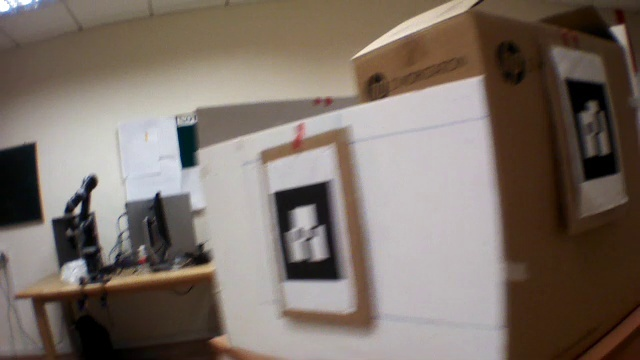
\includegraphics[width=\linewidth]{figures/fiducial/setup_artag/output_79.jpg}
\end{subfigure}
\begin{subfigure}[b]{0.24\textwidth}
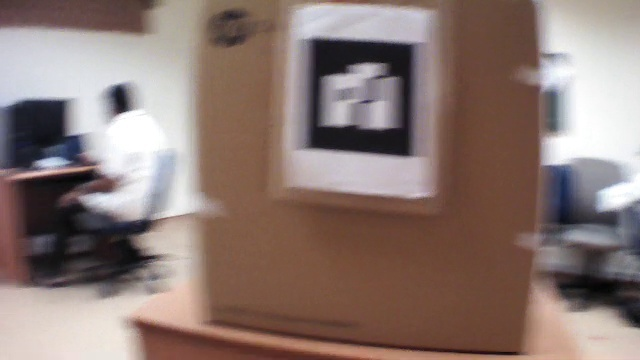
\includegraphics[width=\linewidth]{figures/fiducial/setup_artag/output_150.jpg}
\end{subfigure}
\begin{subfigure}[b]{0.24\textwidth}
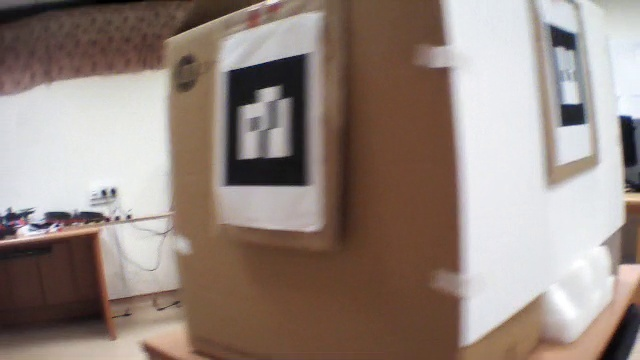
\includegraphics[width=\linewidth]{figures/fiducial/setup_artag/output_194.jpg}
\end{subfigure}
\begin{subfigure}[b]{0.24\textwidth}
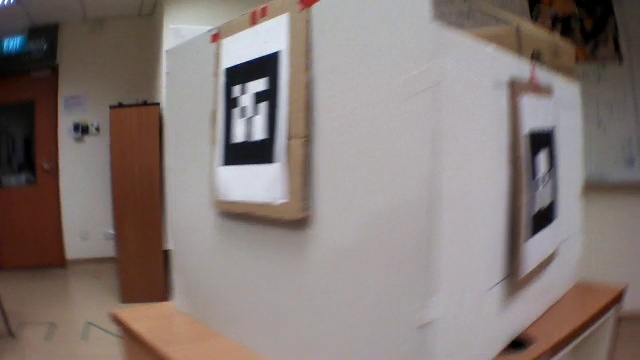
\includegraphics[width=\linewidth]{figures/fiducial/setup_artag/output_480.jpg}
\end{subfigure}\\
\begin{subfigure}[b]{0.24\textwidth}
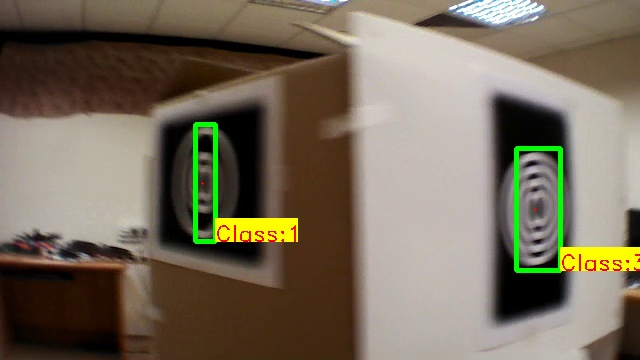
\includegraphics[width=\linewidth]{figures/fiducial/setup_our/output_6/output_514.jpg}
\end{subfigure}
\begin{subfigure}[b]{0.24\textwidth}
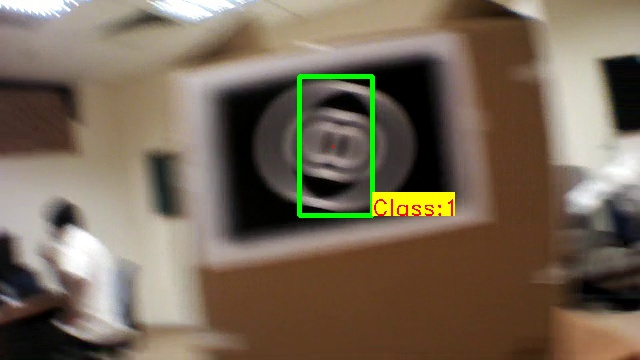
\includegraphics[width=\linewidth]{figures/fiducial/setup_our/output_2/output_64.jpg}
\end{subfigure}
\begin{subfigure}[b]{0.24\textwidth}
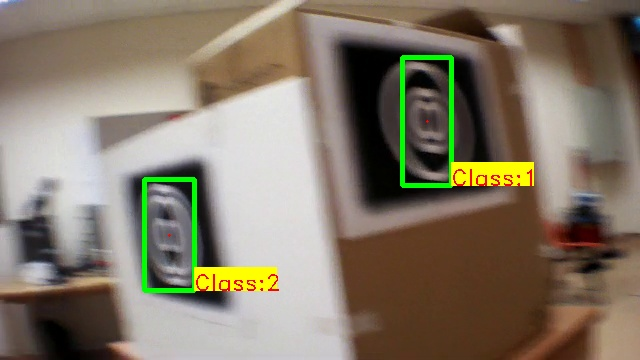
\includegraphics[width=\linewidth]{figures/fiducial/setup_our/output_2/output_35.jpg}
\end{subfigure}
\begin{subfigure}[b]{0.24\textwidth}
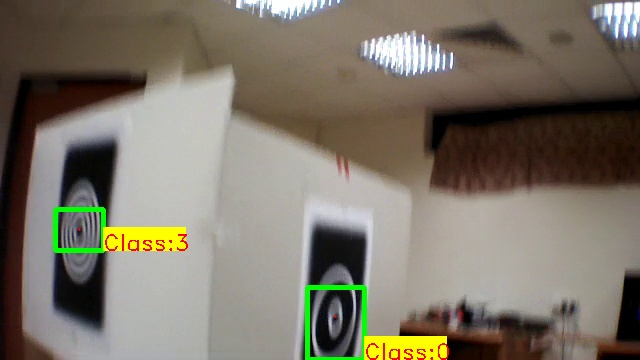
\includegraphics[width=\linewidth]{figures/fiducial/setup_our/output_6/output_943.jpg}
\end{subfigure}
\caption[Comparison of ARTag and our fiducial when quadcopter is
  revolving around our setup]{Comparison of ARTag and our fiducial when quadcopter is
  revolving around our setup. 
\textbf{Top} ARTags are not recognized, shown by an absence of green rectangles.
\textbf{Bottom} In similar conditions, proposed fiducials are successfully
recognized. The overall recognition rate of proposed fiducials is 90\% while that
of ARTags is around 60\%. }
\label{fig:fiducials_result}
\end{figure}
	
\section{Organization of the thesis}
The remainder of the thesis is organized as follows:\\

\noindent \textbf{Chapter 2} explains the details of a quadcopter focusing on
control and navigation aspects. Here, we also present previously published work
in the area of mosaicing, autonomous navigation of quadcopter as well as
fiducials. We use this chapter as an opportunity to establish and contrast the
scope of this thesis with respect to prior art.\\

\noindent \textbf{Chapter 3} elaborates our proposed method for mosaicing
scenes with vacant spaces using quadcopter. Proposed method fuses positional
information from quadcopter with images to first, find out the position from which each
image is taken and accordingly sort the images in two dimensional grid; second,
use positional information to join two adjacent images which have very few features
in common (and hence cannot be stitched using the homography-based method).\\

\noindent \textbf{Chapter 4} provides an overview of our approach
for imaging multiplanar scenes through quadcopter. Issues such as detection of
multiplanar bounded regions and path planning for efficient imaging of multiplanar scenes
are addressed.\\

\noindent \textbf{Chapter 5} elaborates on our design of blur
resilient fiducial for identification of objects under a heavy motion blur. We
have also proposed algorithm for robust recognition of our blur resilient
fiducial in this chapter.\\
 
 \noindent \textbf{Chapter 6} concludes the thesis by summarizing our
 contributions.
  We have also discussed possible ways to extend some of the ideas proposed in this thesis.

\chapter{Literature Survey}
\label{ch:quadcopter}
In this chapter, we will familiarize with a quadcopter, its components, and
technical specifications. We will also discuss the prior work related to
mainly three areas: control and navigation of quadcopter, mosaicing, and
fiducial based tracking. 
\section{Quadcopter}
The necessity for flying device with greater maneuverability and hovering
ability led to the creation of a quadcopter. A quadrocopter or quadcopter  is a
multirotor helicopter that is lifted and propelled by four rotors. The
four-rotor design allows quadcopters to be relatively simple in design yet
highly reliable and maneuverable. The quadcopter  is a  symmetrical vehicle which
has four rods with propellers connected to rotors  at each end. Two diagonally
opposite propellers rotate in clockwise(CW) direction while remaining  two
rotate in counterclockwise(CCW) direction as shown in
Figure~\ref{fig:quadcopter}(Middle). This is done in order to balance the
torque generated by each pair of rotors. The angular movement (roll-pitch-yaw)
around three axes coordinate system of the quadcopter is shown in
Figure~\ref{fig:quadcopter}(Right).


\begin{figure}[b!]
  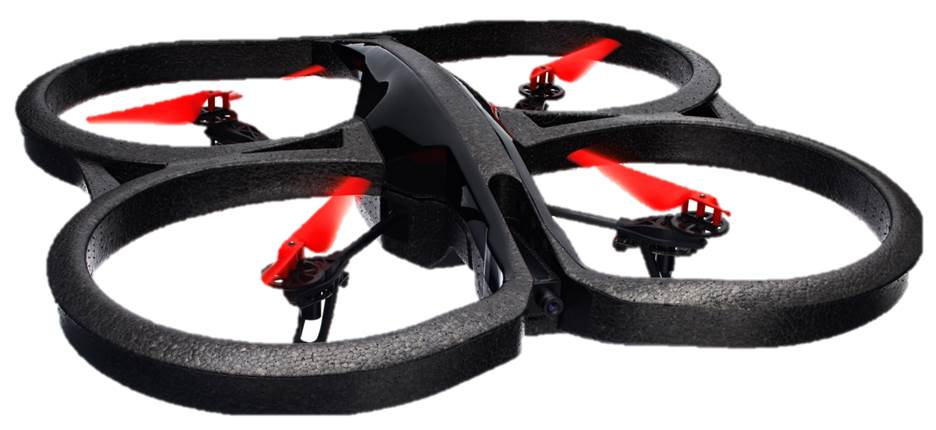
\includegraphics[width=0.3\linewidth]{images/ardrone2}	
  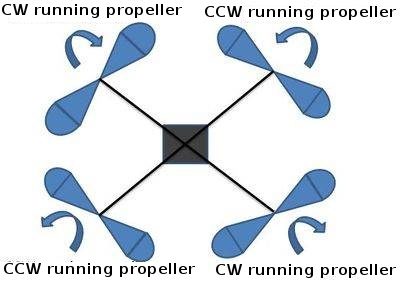
\includegraphics[width=0.34\linewidth]{images/quadrotor}
  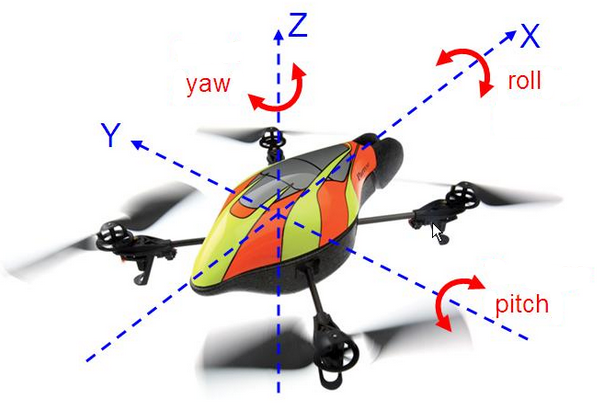
\includegraphics[width=0.34\linewidth]{images/rpy}
  \caption[Quadcopter Motions]{Left: Sample quadcopter, Parrot's ARDrone 2.0.
  Middle: Direction of propeller movement of quadcopter. Right: Rotation of
  quadcopter along three axes. [Picture Courtesy: Google image search]}
  \label{fig:quadcopter}
\end{figure}

The speed of each rotor can be independently varied through onboard flight
controller to achieve various controls. For example, if we would like to hover
the quadcopter, the thrust generated by all rotors should match the weight of the
quadcopter. If we want to move in any direction, then controller tilts the
quadcopter on that side by increasing the speed of rotors on another side. The
horizontal component of the thrust will move the quadcopter in that direction.
If we want to rotate the quadcopter around the z-axis, i.e., to change its yaw,
controller imbalances the torque purposefully by increasing the speed of rotors on
one diagonal. For e.g., if we increase the speed of rotors which are rotating in
clockwise direction, quadcopter will turn in counterclockwise direction.
This is illustrated in Figure~\ref{fig:quadcopterMotion}.

\begin{figure}[h!]
  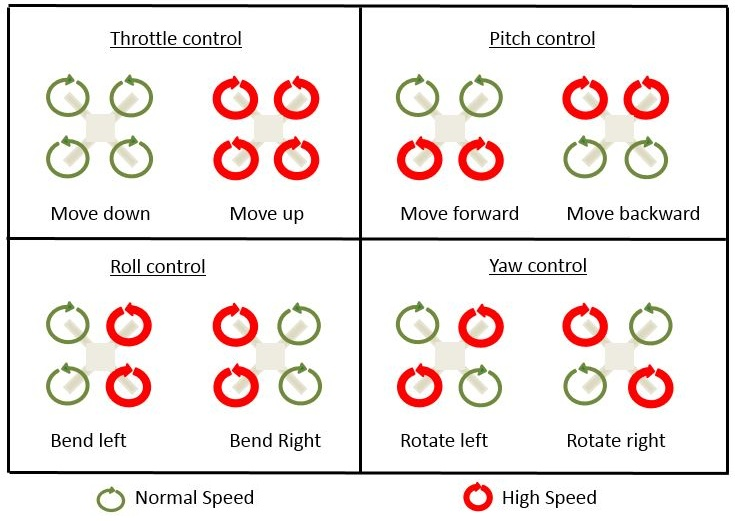
\includegraphics[width=\textwidth]{images/quadcopterMotion.jpg}
  \caption[Speed control of rotors for quadcopter's motion]{Speed control of
  rotors for quadcopter's motion.
  (Left-Top): Speed of all rotors is increased/decreased to move
  quadcopter up/down.
  (Right-Top): To move quadcopter in forward/backward direction, we increase
  speed of rear/front rotors.
  (Left-Bottom): To move quadcopter in left/right direction, we increase
  speed of right/left rotors.
  (Right-bottom): To rotate quadcopter in clockwise direction, we increase speed
  of rotors moving in counterclockwise direction and vice-versa. 
   [Picture Courtesy: Google image search]}
  \label{fig:quadcopterMotion}	
\end{figure}

The quadcopter mainly contains three subsystems: Inertial Measurement Unit (IMU),
Imaging system and Communication system all connected to Central Processing
Unit, an ARM processor. IMU is responsible for getting the pose of a quadcopter.
The imaging system deals with capture and storage of images of the surrounding
environment. Communication system handles interfacing between quadcopter and
client device. Here, we have given details of Parrot's AR Drone 2.0 as we are
using the same for our experiments. Though components will remain mostly same across
different quadcopters, technical specifications (e.g., image resolution) may
vary across various models.

\subsection{Inertial Measurement Unit (IMU)}
Every quadcopter has Inertial Measurement Unit (IMU) onboard in order to maneuver
quadcopter in a controlled way. IMU is an electronic device which measures forces
acted upon the body of a quadcopter. It comprises of 3-axis accelerometer, 3-axis
gyroscope, 3-axis magnetometer, and ultrasound altimeter (also called as sonar).
Accelerometer measures acceleration of quadcopter along 3 axes while gyroscopes
measure angular movement around 3 axes, i.e., roll, pitch, and yaw. Magnetometer
measures angular movement with respect to the magnetic axis of the earth, to get
the absolute angle from magnetic axis. Sonar measures quadcopter's
height from the ground.

Sometimes IMU also has a pressure sensor to measure the air-pressure around the
device. It is helpful in checking if there is a strong wind so that
onboard flight controller can take the corrective action to stabilize the
quadcopter. 

IMU provides us information about linear as well as angular accelerations. This
information is later used to estimate the pose of the quadcopter. However, due
to various factors such as noisy measurements, environmental disturbances, the
estimated pose may be completely off.
 
\subsection{Imaging System}
Parrot's ARDrone 2.0 has two cameras, front camera with a wide-angle lens
($92^{\circ}$ diagonal) to capture images with HD resolution (1280 $\times$ 720
pixels) at 30 FPS, while vertical camera (pointing downwards) having QVGA
resolution (320 $\times$ 240) at 60 FPS used for measuring ground speed.
Though front camera can capture the images at HD resolution, it can transmit
images over Wi-Fi at only  lower resolution (640 $\times$ 360 pixels). Hence, we
need to use USB storage device on quadcopter to store a video streamed by the
quadcopter camera. 

\subsection{Communication System}
The AR.Drone 2.0 can be controlled from any client device supporting WiFi. The 
process followed is:
\begin{enumerate}
  \item The AR.Drone creates a WiFi network with an SSID usually named
adrone2\_xxx (where xxx is manufacture date in YYYYMMDD format) and self
allocates a free, odd IP address (typically 192.168.1.1).

   \item The user connects the client device to this SSID network.
   \item The client device requests an IP address from the drone DHCP server.
   \item The AR.Drone DHCP server grants the client with an IP address which is
   the drone's own IP address plus a number between 1 and 4 e.g., 192.168.1.3.
   \item The client device can start sending requests (Land, Takeoff, etc.) to
   the AR.Drone IP address and its services ports.
\end{enumerate}

ARDrone 2.0 can be controlled from the client device through 3 main communication
services: 
\begin{itemize}
\item \textit{AT} commands for control and configuration are sent on UDP
port 5556.
\item Information about the drone (like its status, position,  speed, 
etc.), called as \textit{navdata}, is sent by the drone to its client on UDP
port 5554.  
\item A video stream is sent by the AR.Drone to the client device on UDP port
5555.
\end{itemize}

Now, we will see prior work done in the field of quadcopter navigation,
mosaicing of scenes, and tracking of a quadcopter.

\section{Control and Navigation of quadcopter}
In this section, we will discuss manual as well as autonomous ways to navigate
a quadcopter, specifically Parrot's ARDrone 2.0.
Parrot has released a mobile app, AR.FreeFlight on iPhone as well as Android
phones for piloting ARDrone. This App can be used to do simple maneuvers such
as going left/right, forward/backward, up/down. It also has a ``Director mode'',
which allows some advanced maneuvers such as circling around itself to take
a panoramic view. But still, it is very difficult to maneuver the drone without
expertise.

\begin{figure}[h!]
  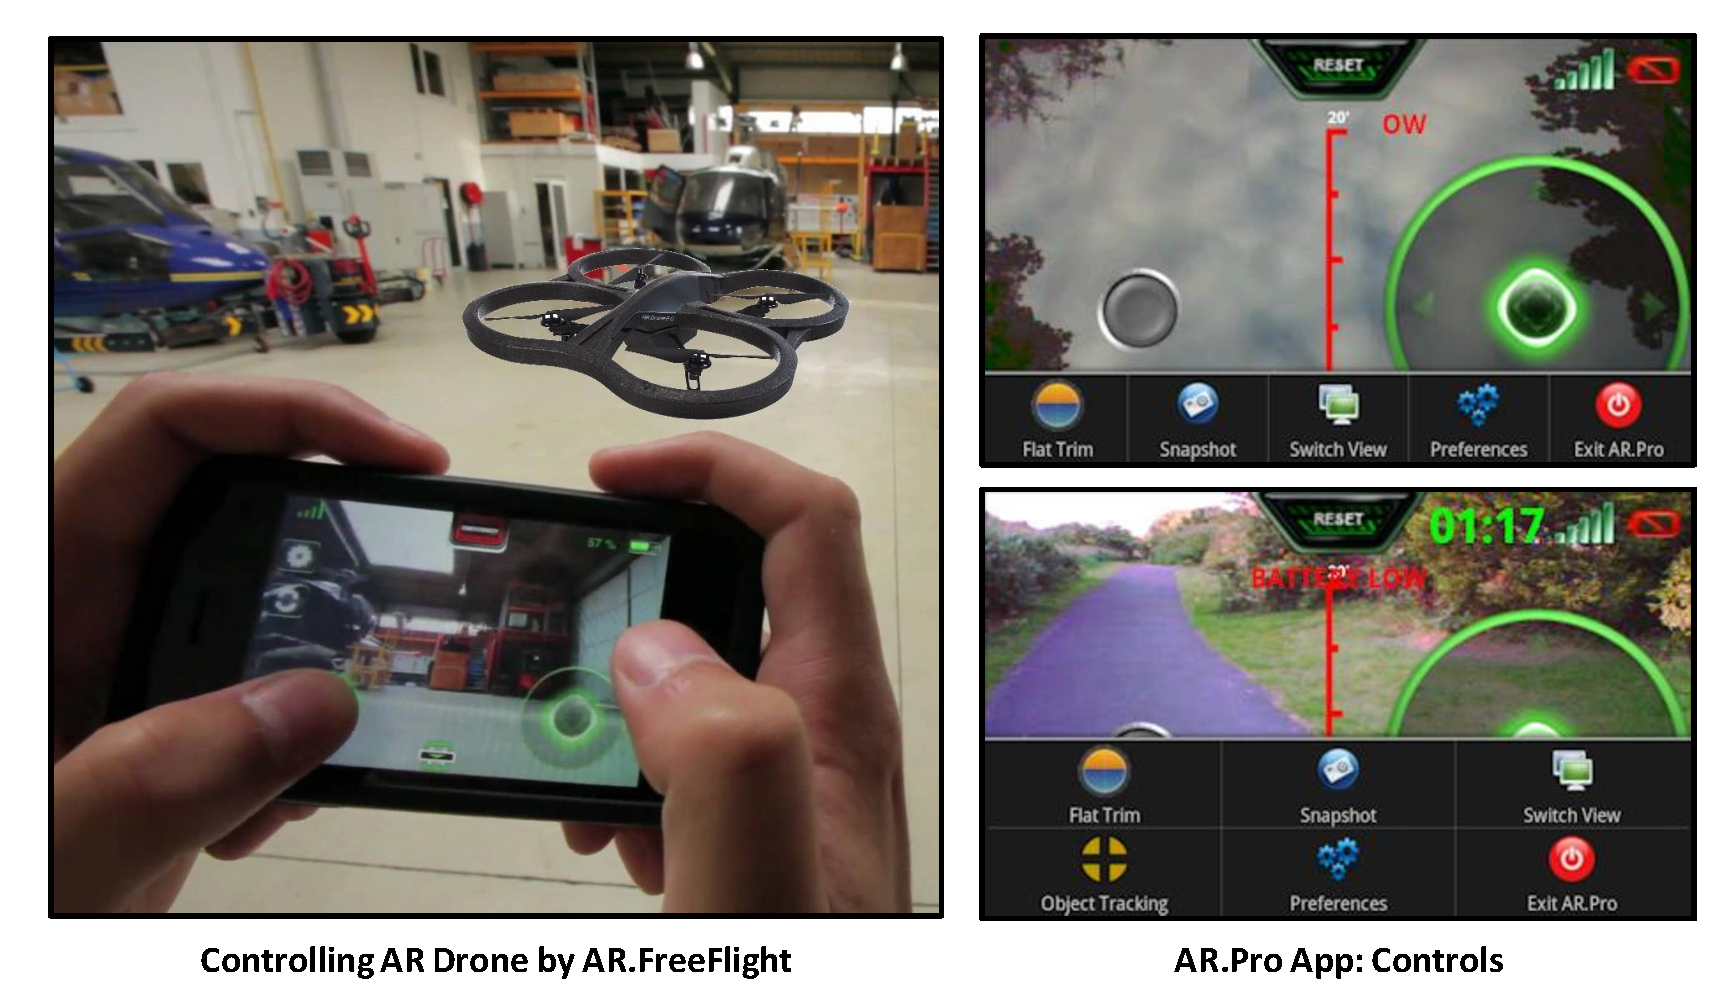
\includegraphics[width=\textwidth]{figures/manualControl}
   \caption[Manual control of Parrot's ARDrone 2.0]{Manual control of Parrot's
  ARDrone 2.0 through smartphone. Left: Parrot's AR.FreeFlight is used to
  control the ARDrone 2.0. 
  Right: Alternatively one may use AR.Pro having advanced features for control.
  [Picture Courtesy: Google image search]}
   \label{fig:manualControl}
\end{figure}

There are also some paid mobile applications such as AR.pro for piloting AR
Drone. AR.pro application has some advanced settings which are not available in
AR.Freeflight e.g., changing WiFi channel, Altitude limiter, Dual Joystick support, etc. All of
these applications involve a lot of manual intervention.  It results in lack of
precision, which is required in an imaging application, e.g., if we want a
quadcopter to complete a rectangular loop and come back to its original
position, it fails to do so.

Some flight controller softwares use add-on GPS for autonomous navigation of
a quadcopter. However in GPS-denied areas e.g., indoor, we cannot use such
softwares. Even in outdoor, we cannot rely on only GPS for accurate
navigation of a quadcopter due to issues like spurious GPS signals, GPS jammers,
etc.

Another way to accurately navigate quadcopter is to use techniques such as
Simultaneous Localization And Mapping(SLAM)\cite{Davison:2007} or Parallel Tracking And
Mapping(PTAM)\cite{klein}. SLAM or PTAM algorithm first builds a 3D map of
surrounding environment and then estimates device's current position.

Engel et al.~\cite{Engel12} have developed a method for navigation of quadcopter
based on PTAM\cite{klein}. Engel et al. have used Extended Kalman Filter (EKF)
to fuse visual observation model with the odometry observation model to estimate
the pose of the quadcopter. They have also developed a method for
correctly estimating the scale of the built 3D map. But, they have not ensured
high scale accuracy which results in an inaccurate 3D map of
the surrounding environment.

\section{Mosaicing of scenes}
Panoramic image stitching (alternatively, image mosaicing) is a
well-studied problem in the field of computer vision.  Representative
works include~\cite{Milgram1975}, \cite{Milgram1977}, \cite{Capel},
\cite{Szeliski1997}, \cite{Brown07}, \cite{Brown03}.  A full discussion
on related works is outside the scope of this thesis. Readers are
referred to~\cite{Szeliski05imagealignment} for an excellent survey.
Given the maturity of this area, there are various freeware as well as
commercial software available for performing image stitching; most
notable are AutoStitch \cite{autostitch}, Microsoft\textsc{\char"13}s Image
Compositing Editor \cite{ICE}, and Adobe\textsc{\char"13}s Photoshop
\cite{photoshop}.

All of these methods are based on a similar strategy of finding
features in each image, matching these features between images, and
then computing pairwise image warps to align them together.  A 
bundle adjustment is often applied to globally refine the alignment.
All of the aforementioned methods assume the imaged scene is planar or
that the camera has been rotated carefully around its center of
projection to avoid parallax.

Brown \etal \cite{Brown05} have used a new type of invariant features
located at Harris corners in discrete scale-space and oriented using a
blurred local gradient for stitching. Eden \etal \cite{Eden} were
able to stitch images with large exposure difference as well as large
scene motion into single HDR quality image without using any
additional camera hardware.

All of the image mosaicing methods work only when there is an
``intersection'' in feature space of images to be stitched. When there
are ``gaps'' (either physical or due to lack of features) between
images to be stitched it is not clear how to perform the
stitching. Structure from Motion methods also rely on the overlap of
features and fail when images have gaps.

\subsection{Mosaicing of Aerial Imagery}
There is a lot of work happened in the area of mosaicing aerial images
captured from UAVs as well as mosaicing of remotely sensed images from satellites.
Representatives of these works are \cite{Yue, Yuanhang, Yahyanejad, Zhu}.
These works use UAVs to image ground scenes from heights (minimum 100 ft.
above from ground). However, we are interested in imaging scenes from a much closer
distance for application such as inspection of walls or towers. Intricacies
involved in imaging such surfaces from the closer distance are different than aerial
imaging. Hence, we \textit{cannot} use methods used for mosaicing of aerial 
imagery in our problem.
\section{Fiducial Markers and Tracking}
Inexpensive quadcopter such as Parrot's AR Drone has very jerky movement. Hence,
it is difficult to track the objects through quadcopter or even the quadcopter
itself. In this section, we will review the prior work done related to the
tracking aspect of the quadcopter.\\

\noindent\textbf{Fiducials:}~Fiducials are often used to evaluate the planning
algorithms given that ground truth positions can be detected by the
quadcopter's camera. Figure~\ref{fig:previous_work} shows a few
examples of existing fiducials.  Many designs use a two
dimensional barcode inside a rectangular grid. One example of such a
fiducial is from the ARToolkit~\cite{ARToolkit02}, a well-known
toolkit used in many augmented reality (AR) applications. Kato and
Billinghurst~\cite{kato-artoolkit} first demonstrated the use of
ARToolkit in various augmented-reality-based applications.

\begin{figure}[b!]
\centering
 \begin{subfigure}[b]{0.29\linewidth}
  \centering
  
\includegraphics[width=0.8\linewidth]{figures/fiducial/intersense.jpg}
  Circular Data Matrix~\cite{NaimarkF02}
 \end{subfigure}\quad
 \begin{subfigure}[b]{0.2\linewidth}
 \centering
  
\includegraphics[width=\linewidth]{figures/fiducial/pattKanji.pdf}
  ARToolkit~\cite{ARToolkit02}
 \end{subfigure}\quad
 \begin{subfigure}[b]{0.2\linewidth}
  \centering
  
\includegraphics[width=\linewidth]{figures/fiducial/ARtag.jpg}
  ARTag\quad~\cite{Fiala05}
 \end{subfigure}\quad
 \begin{subfigure}[b]{0.2\linewidth}
  \centering
  
\includegraphics[width=\linewidth]{figures/fiducial/pifiducial.jpg}
  PiTag\quad~\cite{Pitag13}
 \end{subfigure}
 %\quad
%  \begin{subfigure}[b]{0.14\linewidth}
%   \centering
%   
\includegraphics[width=\linewidth]{figures/fiducial/our_fiducial.jpg}
%   Our Fiducial
%  \end{subfigure}
 \caption[Prior fiducials]{Prior fiducials. While each code has its pros and
 cons depending on the environment, no prior code is expressly designed to be
 recognized under motion blur.}
 \label{fig:previous_work}
\end{figure}


Fiala~\cite{Fiala05} proposed a fiducial termed, ARTag, which is a
bi-tonal system consisting of a square border and an interior
6$\times$6 grid of black or white cells. The improvement of the ARTag
compared to the ARToolkit lies in the detection of corners instead of
detection of lines to find possible patterns.  This proved to be more
efficient than \cite{ARToolkit02} in terms of recognition rate as well
as the number of different patterns which can be created.  {\it The
reliance on both line and corner detection, however, hampers
recognition under motion blur.}

There were also attempts to use circular patterns instead of
rectangular.  Gatrell et al.~\cite{concentric} used concentric circles
for monocular pose estimation as well as object identification. Cho et
al.~\cite{Cho:2001,Cho97fastcolor} have used multicolor rings instead
of black and white rings~\cite{concentric} to increase a possible number
of fiducials.  These multicolor rings are used in wide area tracking
in large-scale applications.  {\it Although based on  concentric rings, these
approaches require the complete ring to be recognized; this is
impractical when the pattern undergoes directional motion blur.}

Naimark and Foxlin~\cite{NaimarkF02} proposed a circular bar code
called the Circular Data Matrix that is beneficial in terms of easy
detection and ability to have a large number of uniquely identifiable
codes.  To address the issue of occlusion, Bergamasco et
al.~\cite{runetag11} proposed the RUNE-tag fiducial by creating a
number of circular dots arranged in circular fashion. RUNE-tags can be
detected even when 50\% of the fiducial area is occluded. Bergamasco
et al.~\cite{Pitag13} proposed the PiTag fiducial, also composed of
circular structures but arranged in a rectangle, to exploit projective
invariant cross-ratio.  This provided similar occlusion resistance as
RUNE-tag but with even less circular dots. {\it All of these techniques,
however, rely on generic feature detection (e.g., circle detection)
and such algorithms break down under motion blur.}\\

%Zhang et al.\cite{Zhang:2002} and Claus et al. \cite{ClausF04} have done
%quite comprehensive comparative study of various fiducial systems with
%respect to processing time, recognition rate and accuracy with
%respect to viewing angle and distance.

\noindent{\textbf{Tracking:}}~~Fiducial detection between successive video
frames can be considered as a tracking problem where the tracked
object is the fiducial.  There is a very large body of research
dedicated to tracking and interested readers are referred
to~\cite{Yilmaz:2006} for a good survey.

Most tracking methods~\cite{Ross:2008, Wu:2009, Perez02, Mei:2009} assume
the image sequence to be blur free. In reality, however, the presence
of motion blur in a video sequence is often unavoidable. To this end,
Wu et al.~\cite{Wu:2011} proposed the Blur-driven Tracker (BLUT)
framework for tracking motion-blurred targets. BLUT is based on the
observation that although motion blur degrades the visual features of
the target, it may also provide useful cues about the movements to help
tracking.

The BLUT framework successfully tracks a blurred target when there is
uniform motion and the position of the tracked object does not change
drastically in successive frames. However, the erratic motion from the
quadcopters, as well as the problem of dropped video frames, makes the task too
problematic for BLUT to successfully track.

In this chapter, we got acquainted with a quadcopter, motion control, its
components. We also have seen limitations of existing methods for quadcopter
travel and imaging.  We will discuss how these limitations are addressed in
upcoming chapters.

\chapter{Mosaicing Scenes with  Vacant Spaces}
\label{ch:vacantSpaces}
\section{Introduction}
Finding features and using them to align images to construct wide
field of view panoramas is one of the success stories of computer
vision.  Virtually all recent consumer cameras have this technology
embedded.  The success of these methods relies significantly on
finding common features in the images that can be used to establish
the appropriate warps to register the images together.

\begin{figure}
  \centering
  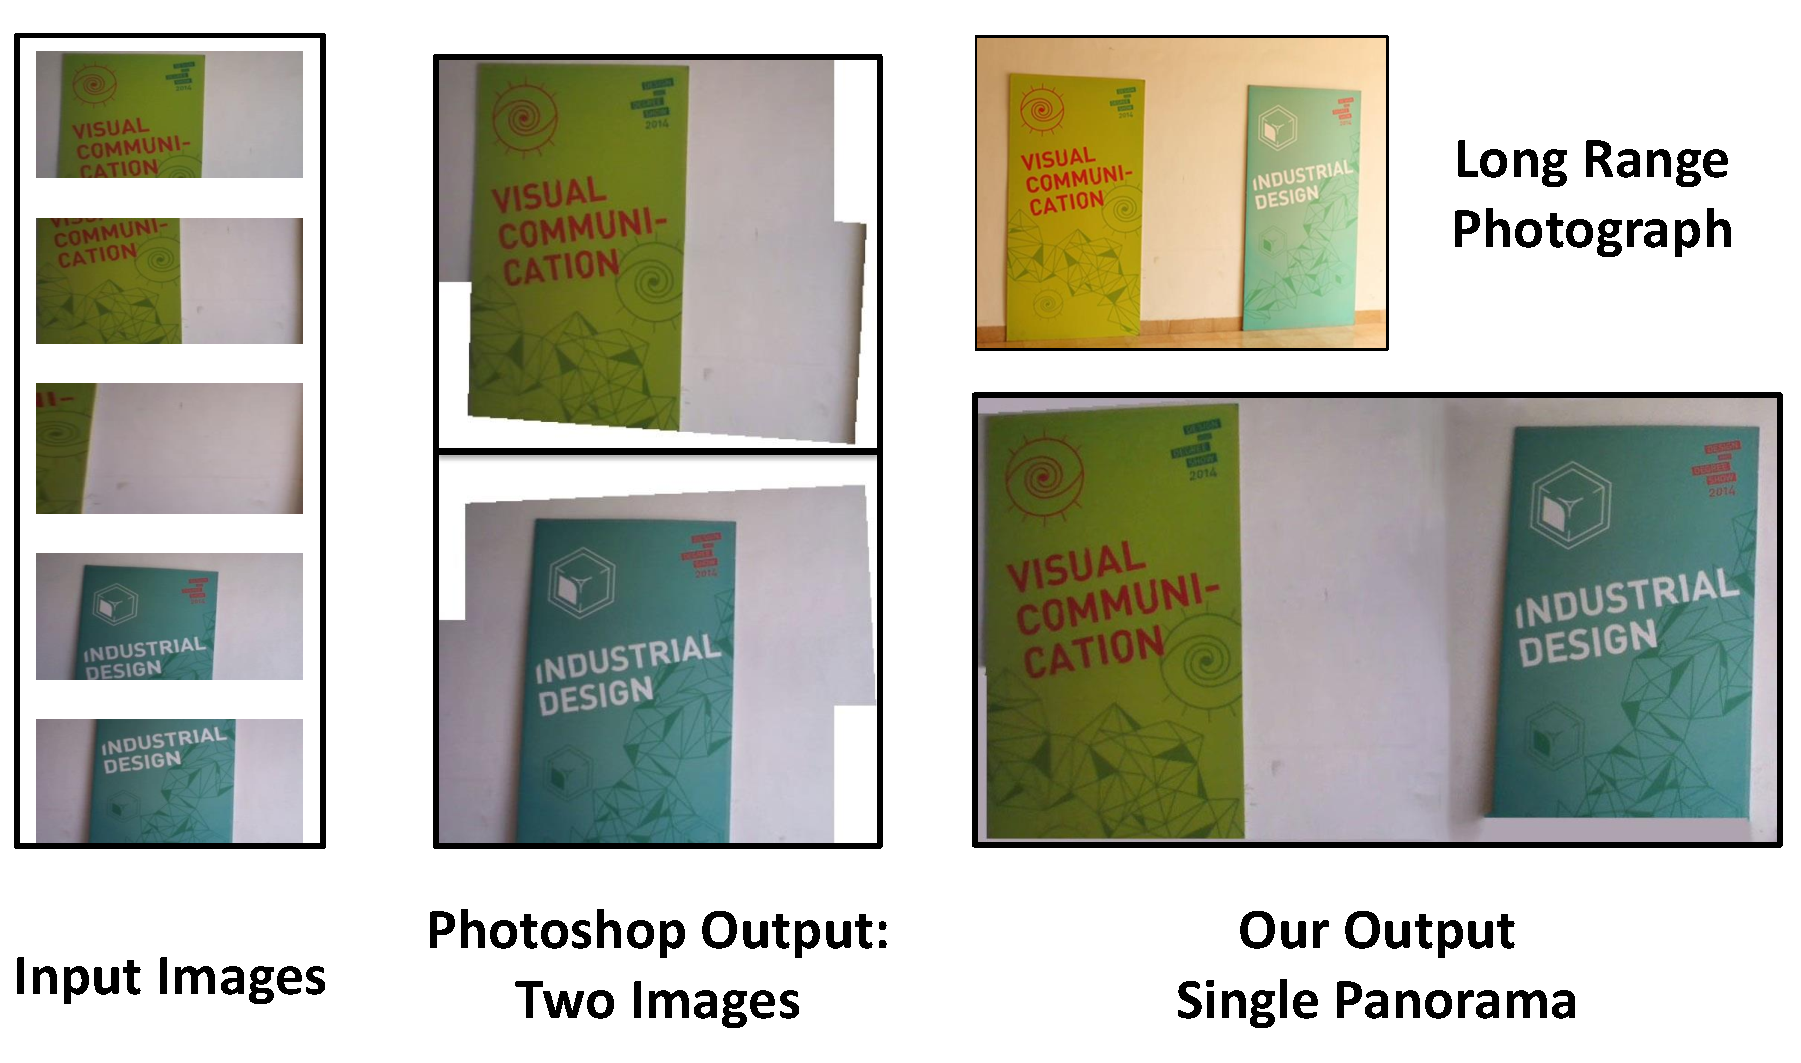
\includegraphics[width=0.8\textwidth]{figures/vacantSpaces/teaser.pdf}
  \caption[Overview]{ \label{fig:vacantTeaser} The long range photograph of a scene
    taken from an SLR camera is shown in top right.  When such a scene
    is probed by a quadcopter, it results in the input images shown on
    the left (color balance is different from the SLR camera).  The
    state of the art methods (middle column) are unable to make a
    \emph{single} mosaic because the vacant space (third picture on
    the left) does not seem to have any matchable features with
    subsequent input images. Our method handles this situation (bottom
    right).  }
\end{figure}

There are scenes, however, that consist of image content that makes
this challenging.  One situation is when the scene needs to be probed
in an orthographic view and is not easily accessible.  Murals on
urban architecture is an example. Another situation is when scene
patterns and texture are repeated (too many similar features in, e.g.,
an outdoor art exhibition).  This can make it challenging for a
matching algorithm to find appropriate matches in large panoramas.  A
related situation is when a scene area simply does not contain
features (too little, or no features, e.g. posters in an event).
Fig~\ref{fig:vacantTeaser} shows an example of this case.  The state of the
art methods are unsatisfactory.  The idea of a moving quadcopter
taking pictures suggests using a Structure from Motion (SfM) paradigm.
However, based on our experiments with Bundler\cite{Snavely06,
  Snavely07} and VisualSFM \cite{Wu13}, we see that the success of SfM
depends very strongly on ``good'' correspondences between input
images, absent in large vacant (featureless) spaces. Specialized -- state of the art -- image stitching 
methods from \cite{Brown03, Brown05} used in tuned software like Adobe 
Photoshop CS6 or AutoStitch \emph{also} do not work as can be seen 
in Figure~\ref{fig:vacantTeaser}.


The goal of this work is to create panoramic images of scenes using a
quadcopter in situations described above. From a vision perspective,
we are excited about a new mosaicing problem containing large
homogeneous vacant spaces.  This results in scene regions that have no
matches between many significant images, and therefore cannot be
aligned using traditional mosaicing methods.


{\bf Key Idea} We propose to solve the vacant space problem by using
an inexpensive off-the-shelf flying device, such as a quadcopter which
can be assumed to contain an inertial measurement unit (IMU) that has
positional information.  The proximity relationship that the resultant
images have, can be used to significantly reduce the search space in
finding matches.  Further, the proximity relationship also allows, in
principle, to vary the parameters involved in feature selection. For
example, if there is a reason to believe that two images are adjacent
horizontally, one can choose to adjust thresholds in feature matching
algorithm to hunt for otherwise elusive matching pairs.

We note that IMU data can be also made available in other devices such
as smartphones.  An autonomously programmed quadcopter, however, is
particularly enticing because of its ability to fly to areas that are
accessible to the human eye, but inaccessible for the human to
reach. Such areas do not lend themselves easily to high-quality
images. 

Further, IMU data, whether on a smartphone or on a quadcopter, cannot
be relied exclusively, or sometimes at all, especially on inexpensive
devices. Our experiments indicate that the roll and pitch angles
(depending on the distances involved) may be completely off, and so
can the physical coordinates.  This is a consequence of the jerky,
swift movements.  Complementing the IMU with information gleaned from
vision algorithms, however, may be a useful practice.

{\bf Contributions} The main technical contribution of this work is
that it improves the state of the art in mosaicing.  We assume that
the imagery is acquired by a quadcopter for the reasons mentioned
above. Sending a battery of images from a quadcopter to an image
mosaicing algorithm such as AutoStitch incapacitates the algorithm
because of the sheer number of images. Sending a sampled version of
images to a manageable number $N$ of images, with $O(N^2)$ possible
areas to match for features, also does not work since the sampled
image contains vacant space.  In this work, we use IMU information
that lends itself to a graceful $O(N)$ algorithm.  Results are
available in the experiments section. In summary, we have a solution to a new problem, and a
faster solution using IMU data.

%{\bf Limitations} 
In this work, we assume that the scene lies on a planar surface, or
approximately planar surface. The quadcopter can also be programmed to
have a viewing angle perpendicular to any desired planar structure.
The standard homography computation is still not possible because of
the vacant spaces. To overcome this, we reduce the mosaicing problem
to the stereo problem and are thus able to complete the panorama.

% The rest of this paper is organized as follows.  In the next section,
% we discuss related work.  Subsequently, we describe the main steps in
% our process, and justify the process in Section~\ref{sec:results} with
% experimental results. (Additional results are available in
% supplementary material.)  The final section discusses future work.

\section{Methodology}

The goal of this work is to compute a panorama of a scene lying on
a planar surface that has regions of vacant spaces.  A schematic for
this problem is shown in Figure~\ref{fig:schematic}. 

\begin{figure}[h!]
  \centering
  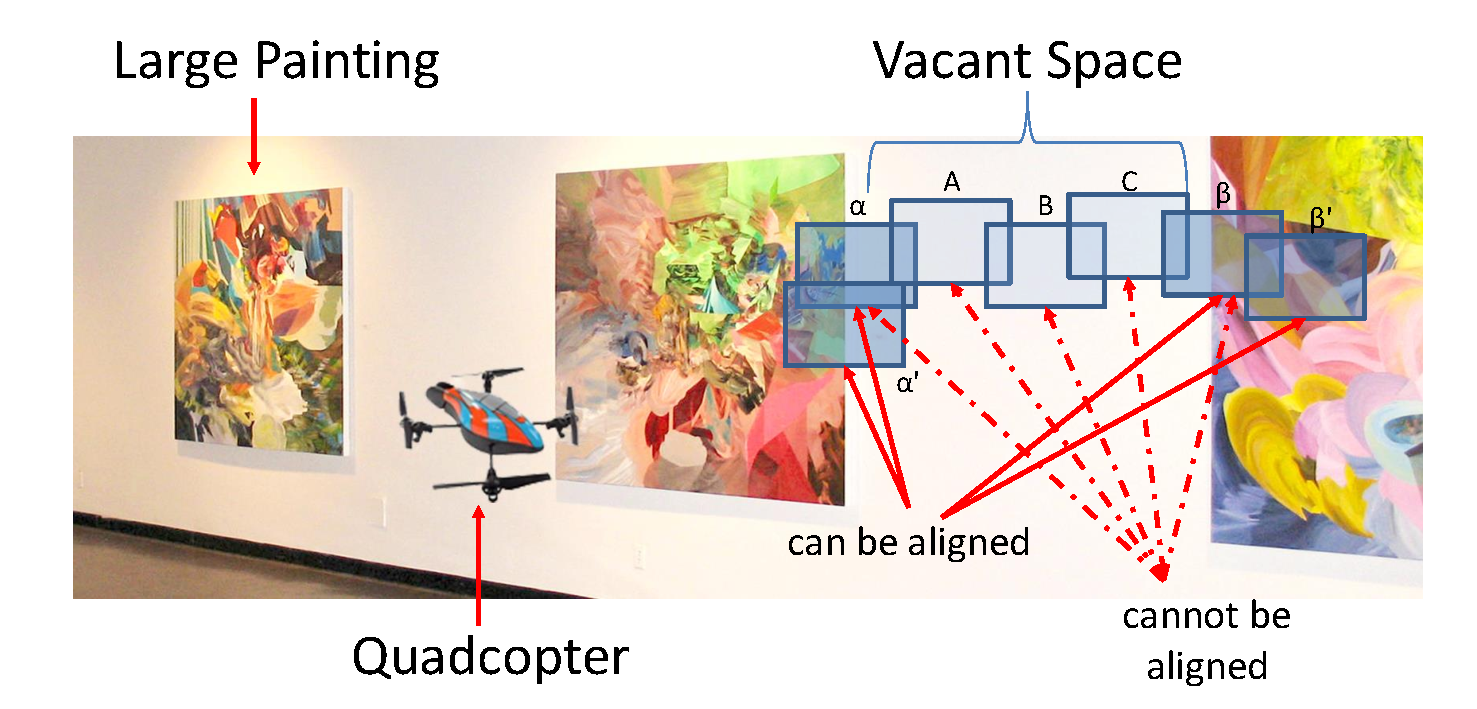
\includegraphics[width=0.8\textwidth]{figures/vacantSpaces/indoor}\\
  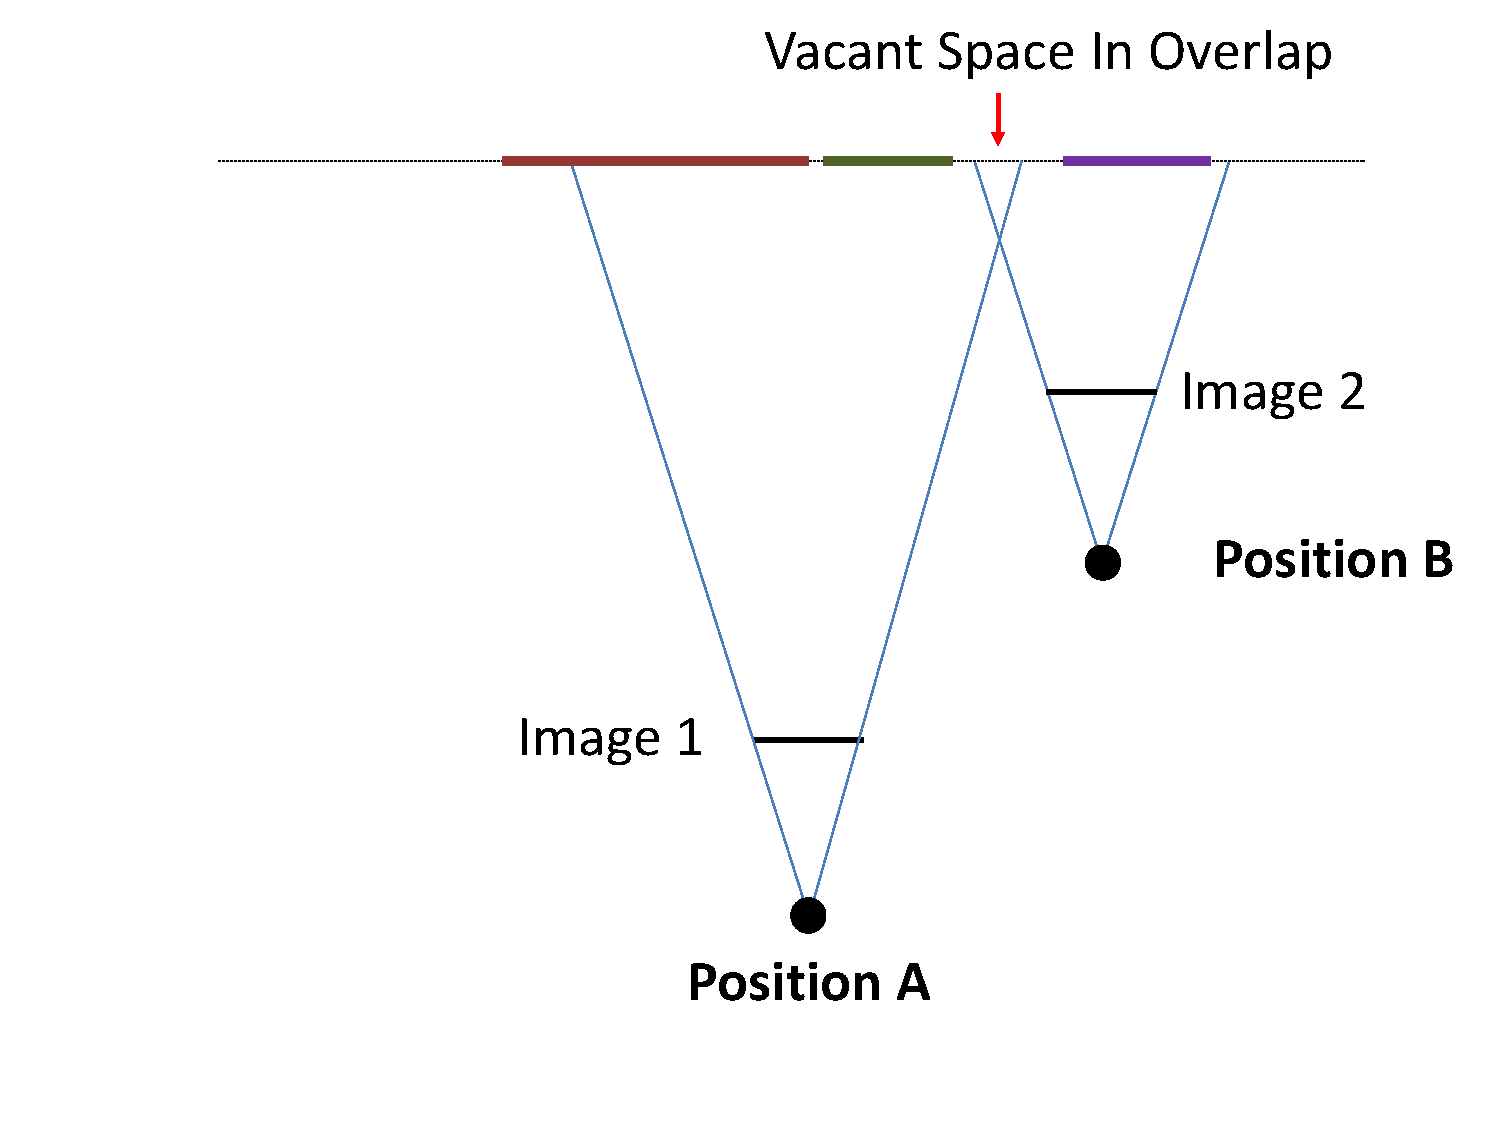
\includegraphics[width=0.8\textwidth]{figures/vacantSpaces/stereoOverlap}\\

  \caption[Problem definition]{ \label{fig:schematic} Problem definition. (Top)
  Vacant spaces are encountered in various scenes.  When individual portions are
    captured by a quadcopter, how does one create the complete mosaic
    given that common features are either not available, or
    confusing? (Bottom) Simplified reduction of the problem to a geometrical structure.
  }
\end{figure}    

The method adopted is pictorially depicted in the overview shown in
Figure~\ref{fig:vacantworkflow} and is described in detail later on.  In
brief, we systematically acquire a video of the scene, reduce the
input video to a manageable number of images, and finally combine the
images acquired from different positions into a mosaic.

\begin{figure}[h!]
  \centering
  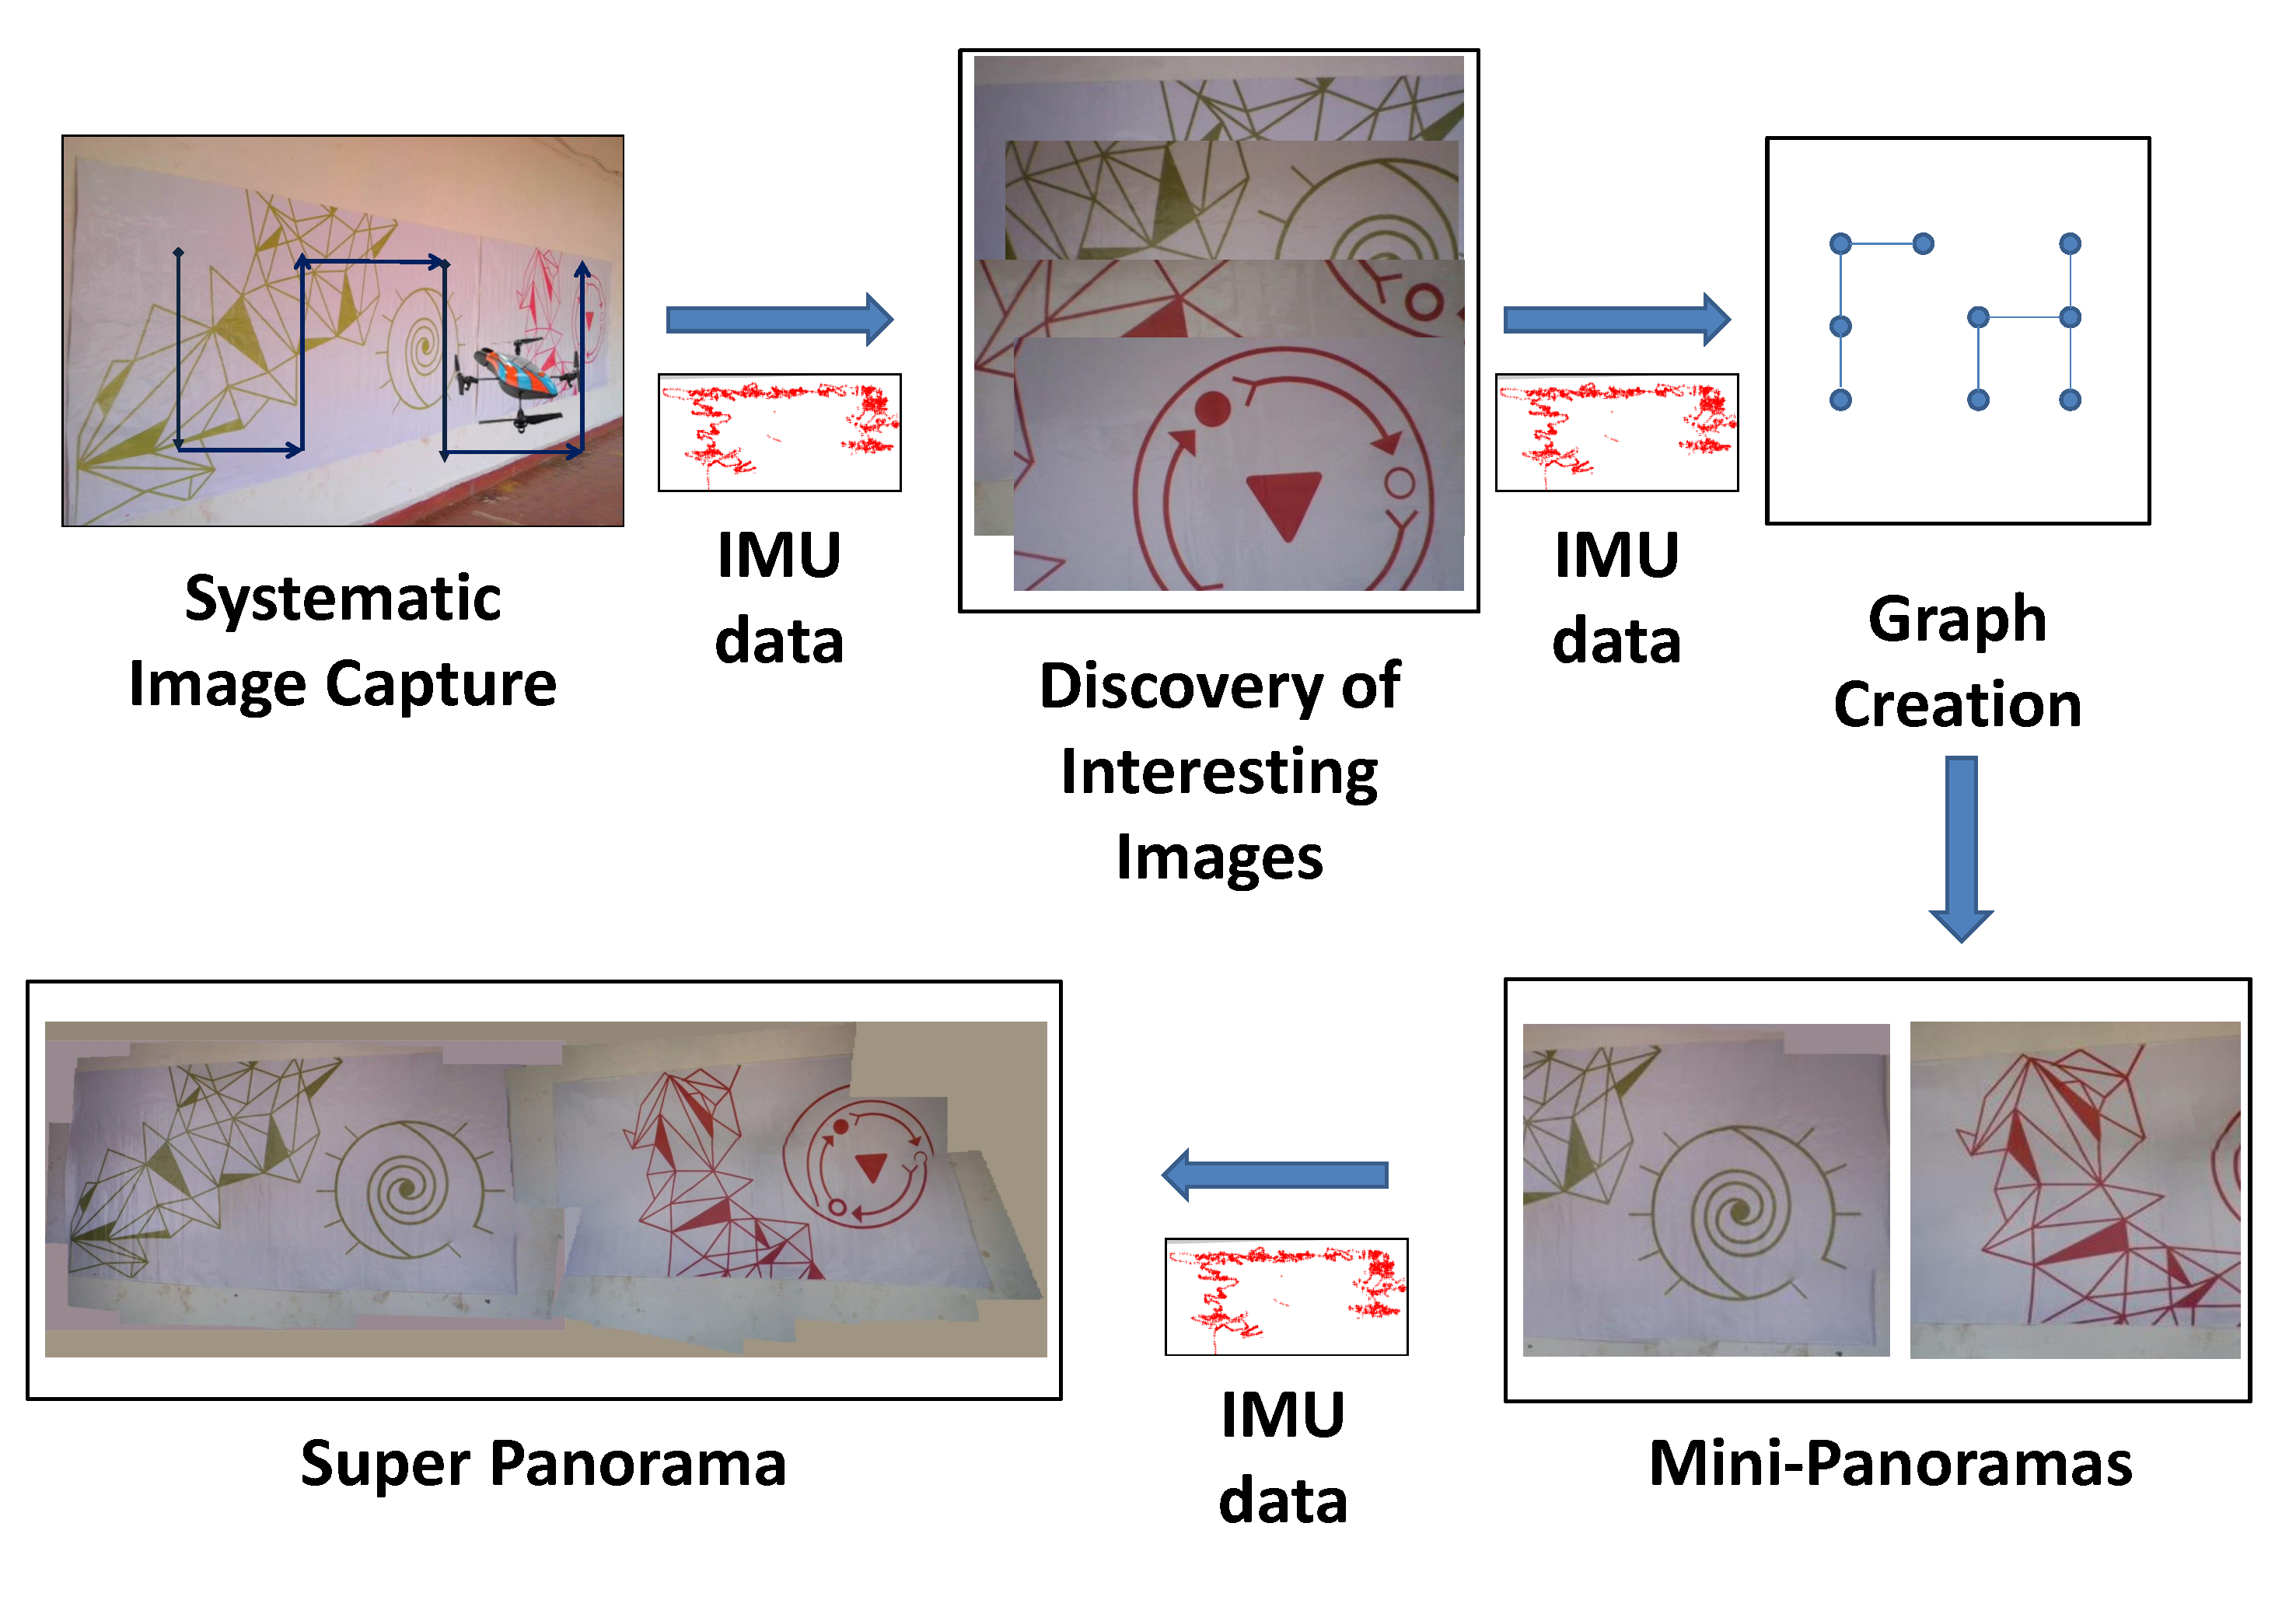
\includegraphics[width=\textwidth]{figures/vacantSpaces/Workflow} 
  \caption[Workflow]{ \label{fig:vacantworkflow} Overview: Input imagery is
    systematically acquired (top left) by a quadcopter.  In the next
    step, interesting images are found by clustering the video into
    regions based on positional data.  A graph is constructed using
    proximal images. For each connected component in a graph, standard
    stitching techniques are used to create mini-panoramas which are
    then joined together into the super-panorama 
    again using IMU data.}
\end{figure}    


\subsection{Video acquisition}
We first dispatch the quadcopter to as close to the scene as
possible. The corners of a rectangular area of interest are provided
to the quadcopter, and it is programmed to traverse the area in a
raster scan fashion.  There are various control aspects involved in
sending a quadcopter; in outdoor areas, the quadcopter is impacted by
the wind and it might lose its way.  The control aspects of the quadcopter
are beyond the scope of this work.  \emph{Note that trying to create a
  mosaic in an incremental linear fashion by combining adjacent frames is
  prone to loss of two-dimensional spatial proximal information. It is also
  computationally overwhelming.}

The quadcopter returns with a video of the scene.  Images extracted
from a short video of about a minute or more overwhelms existing
mosaicing software, such as AutoStitch or Adobe Photoshop.  In the
rest of this section, we use AutoStitch to indicate the state of the art
stitching programs such as AutoStitch, Photoshop, etc.

\subsection{Acquiring interesting images}
\label{sec:selection}
Our goal in this step is to reduce the amount of input data and
produce a set of interesting images.  In other words, we wish to
convert a video into an album of images.  The key difference between
our problem and standard albumization \cite{Aner, Lee} is the use of
positional information.  A standard quadcopter has an inertial
measurement unit (IMU) that, after calibration, may give reasonably
accurate information of positions. Using positional information it is
possible to cluster the images and sort the images into an $m\times
n$ grid.  The number of cluster centers is automatically determined
using the agglomerative bottom-up hierarchical clustering method
\cite{Lior}, with the additional requirement that the whole scene
(represented by the positional data) is covered.

{\bf Clustering Details} We assume that each IMU data position
corresponds to an image of definite fixed dimensions.  Consider each
position of the IMU data to be a leaf node. Two nodes are greedily
combined based on the closest Euclidean distance, and replaced with an
internal node; the position of the internal node is set to be the
centroid of the two nodes, and each internal node now corresponds to a
virtual image of the same size taken by a virtual quadcopter.  The
algorithm recursively merges all the nodes till we end up with a root.
In the next phase, we produce cluster centers; a set of nodes is
considered for being the output as cluster centers if the union of
these nodes completely cover the scene. From the bottom-up
construction, it is clear that the root will represent a single
position, and thus a single virtual image, and will not cover the
scene.  At the other extreme, the set of all leaf nodes \emph{will}
cover the scene. To resolve this, during the calibration phase, we
pre-decide the minimum distance between two centers of projection to
have the least overlap. This is used as the threshold in the clustering
algorithm.  Once cluster centers are found, we pick the leaf node
which is closest to the cluster center to find a real image. This
process is schematically shown in Figure~\ref{fig:selection}.

If we had no IMU information, one may consider selecting a
set of interesting images using any appearance-based method such as
optical flow or feature selection.  However, due to the jerky and
uneven motion of the quadcopter, such measures do not prove to be
sufficient. On the other hand, on inexpensive quadcopters, we have
encountered several cases of erroneous positional information (we note
here that image computations are not on-board the quadcopter and IMU
information is transmitted via WiFi to a host computer).  

% We believe
% that combination of standard vision-based clustering method with the
% clustering based on positional information can be used to either drop
% frames, or to correctly include frames based on image content.

\begin{figure}[t!]
  \centering
  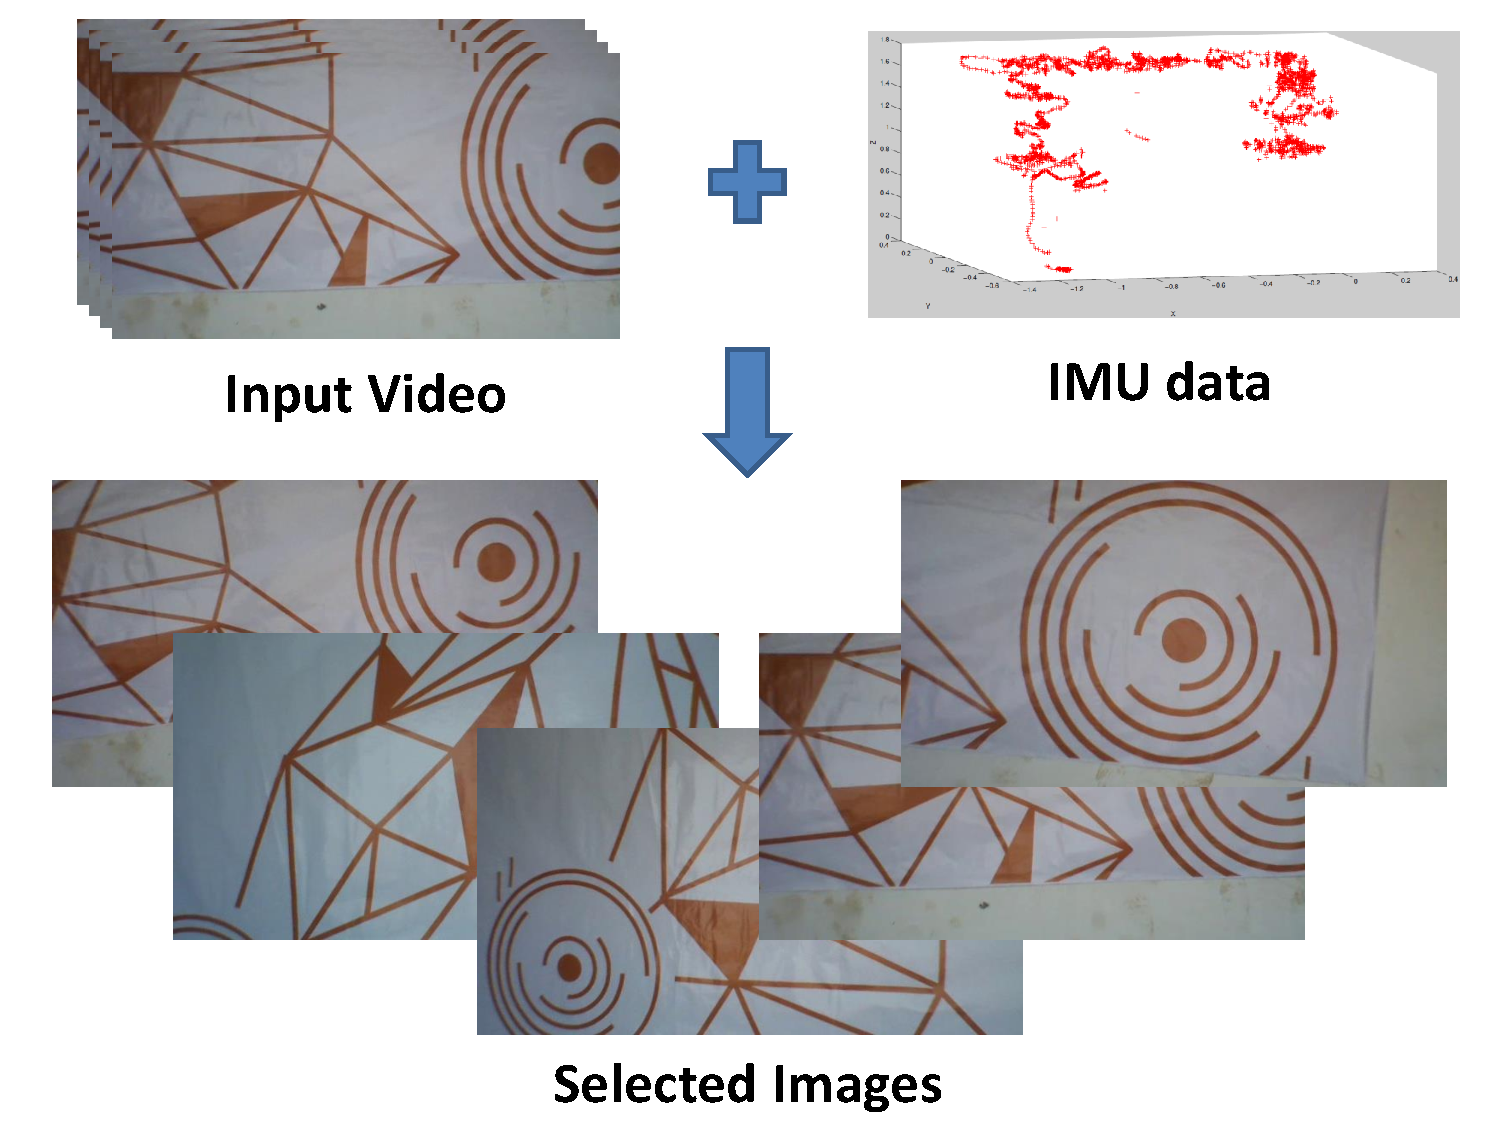
\includegraphics[width=0.42\textwidth]{figures/vacantSpaces/selection} 
  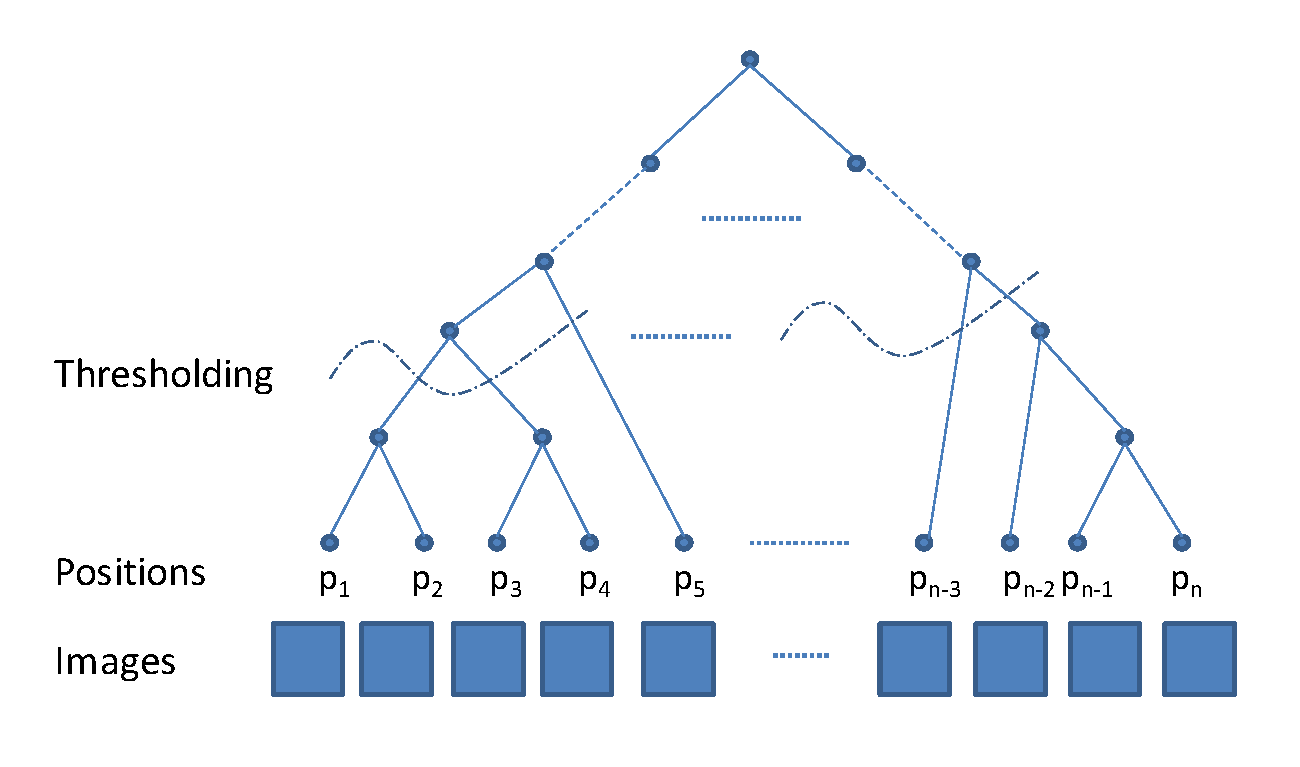
\includegraphics[width=0.56\textwidth]{figures/vacantSpaces/clustering}
  \caption[Selection of Images]{ \label{fig:selection} Left:We align the image
  stream with IMU data, and then transform the video into a set of interesting
    images with a clustering algorithm. Right: Hierarchical clustering is done
    on the positional data to find out the optimal number of positions which
    `encompasses' the scene. Threshold based on the average distance of the
    quadcopter from the plane is used to prune the tree.}
\end{figure}    

In practice, the number of cluster centers for the scenes we have
covered is now within the capacity of AutoStitch.  As mentioned in the
introduction, as long as there are sufficiently varying and
``matchable'' features, AutoStitch is able to perform a reasonable
result.  However, if there are very few features in the overlapping region
of two images, then the output is not acceptable. This situation will
arise when there is vacant space between two pictures.

{\bf Time complexity} AutoStitch has not been designed
to use positional information. As a result, if there are $N$ input
images, the program has to consider possible matches in approximately
$O(N^2)$ set of areas.  Our program is able to mosaic in an $O(N)$
fashion.

{\bf Mini-Panoramas} Specifically, we assume at this point that the
interesting photos are available in the form of a $m \times n$
grid. First, we find SURF \cite{Bay} features for each image in a
grid. Next, we use Best of Nearest Neighbor matcher (from the OpenCV
library) with Random Sample Consensus (RANSAC) \cite{Fischler1981} to
find geometrically consistent matches between neighborhood images
inside grid.  We create a graph with images being nodes and add an
edge between two nodes if there are sufficient matches. We have to
recall at this point that if there are ``vacant spaces'' there will
not be enough features for successful matches; the graph will end up
with multiple (disconnected) components.  We next compute multiple
spanning trees for the various components. Given a spanning tree, the
center of the spanning tree is a node from which the distance to all
other nodes is minimal \cite{Kocay}. Next, we calculate the homography
of each image with respect to spanning tree center.  Finally, for each
spanning tree, we stitch all pictures within the spanning tree to
create a mini-panorama using the computed homographies by warping all
images with reference to the image at spanning tree center. The
spanning tree is an $O(N)$ structure. The process is described in
Figure~\ref{fig:graph}.

\begin{figure}[t!]
  \centering
  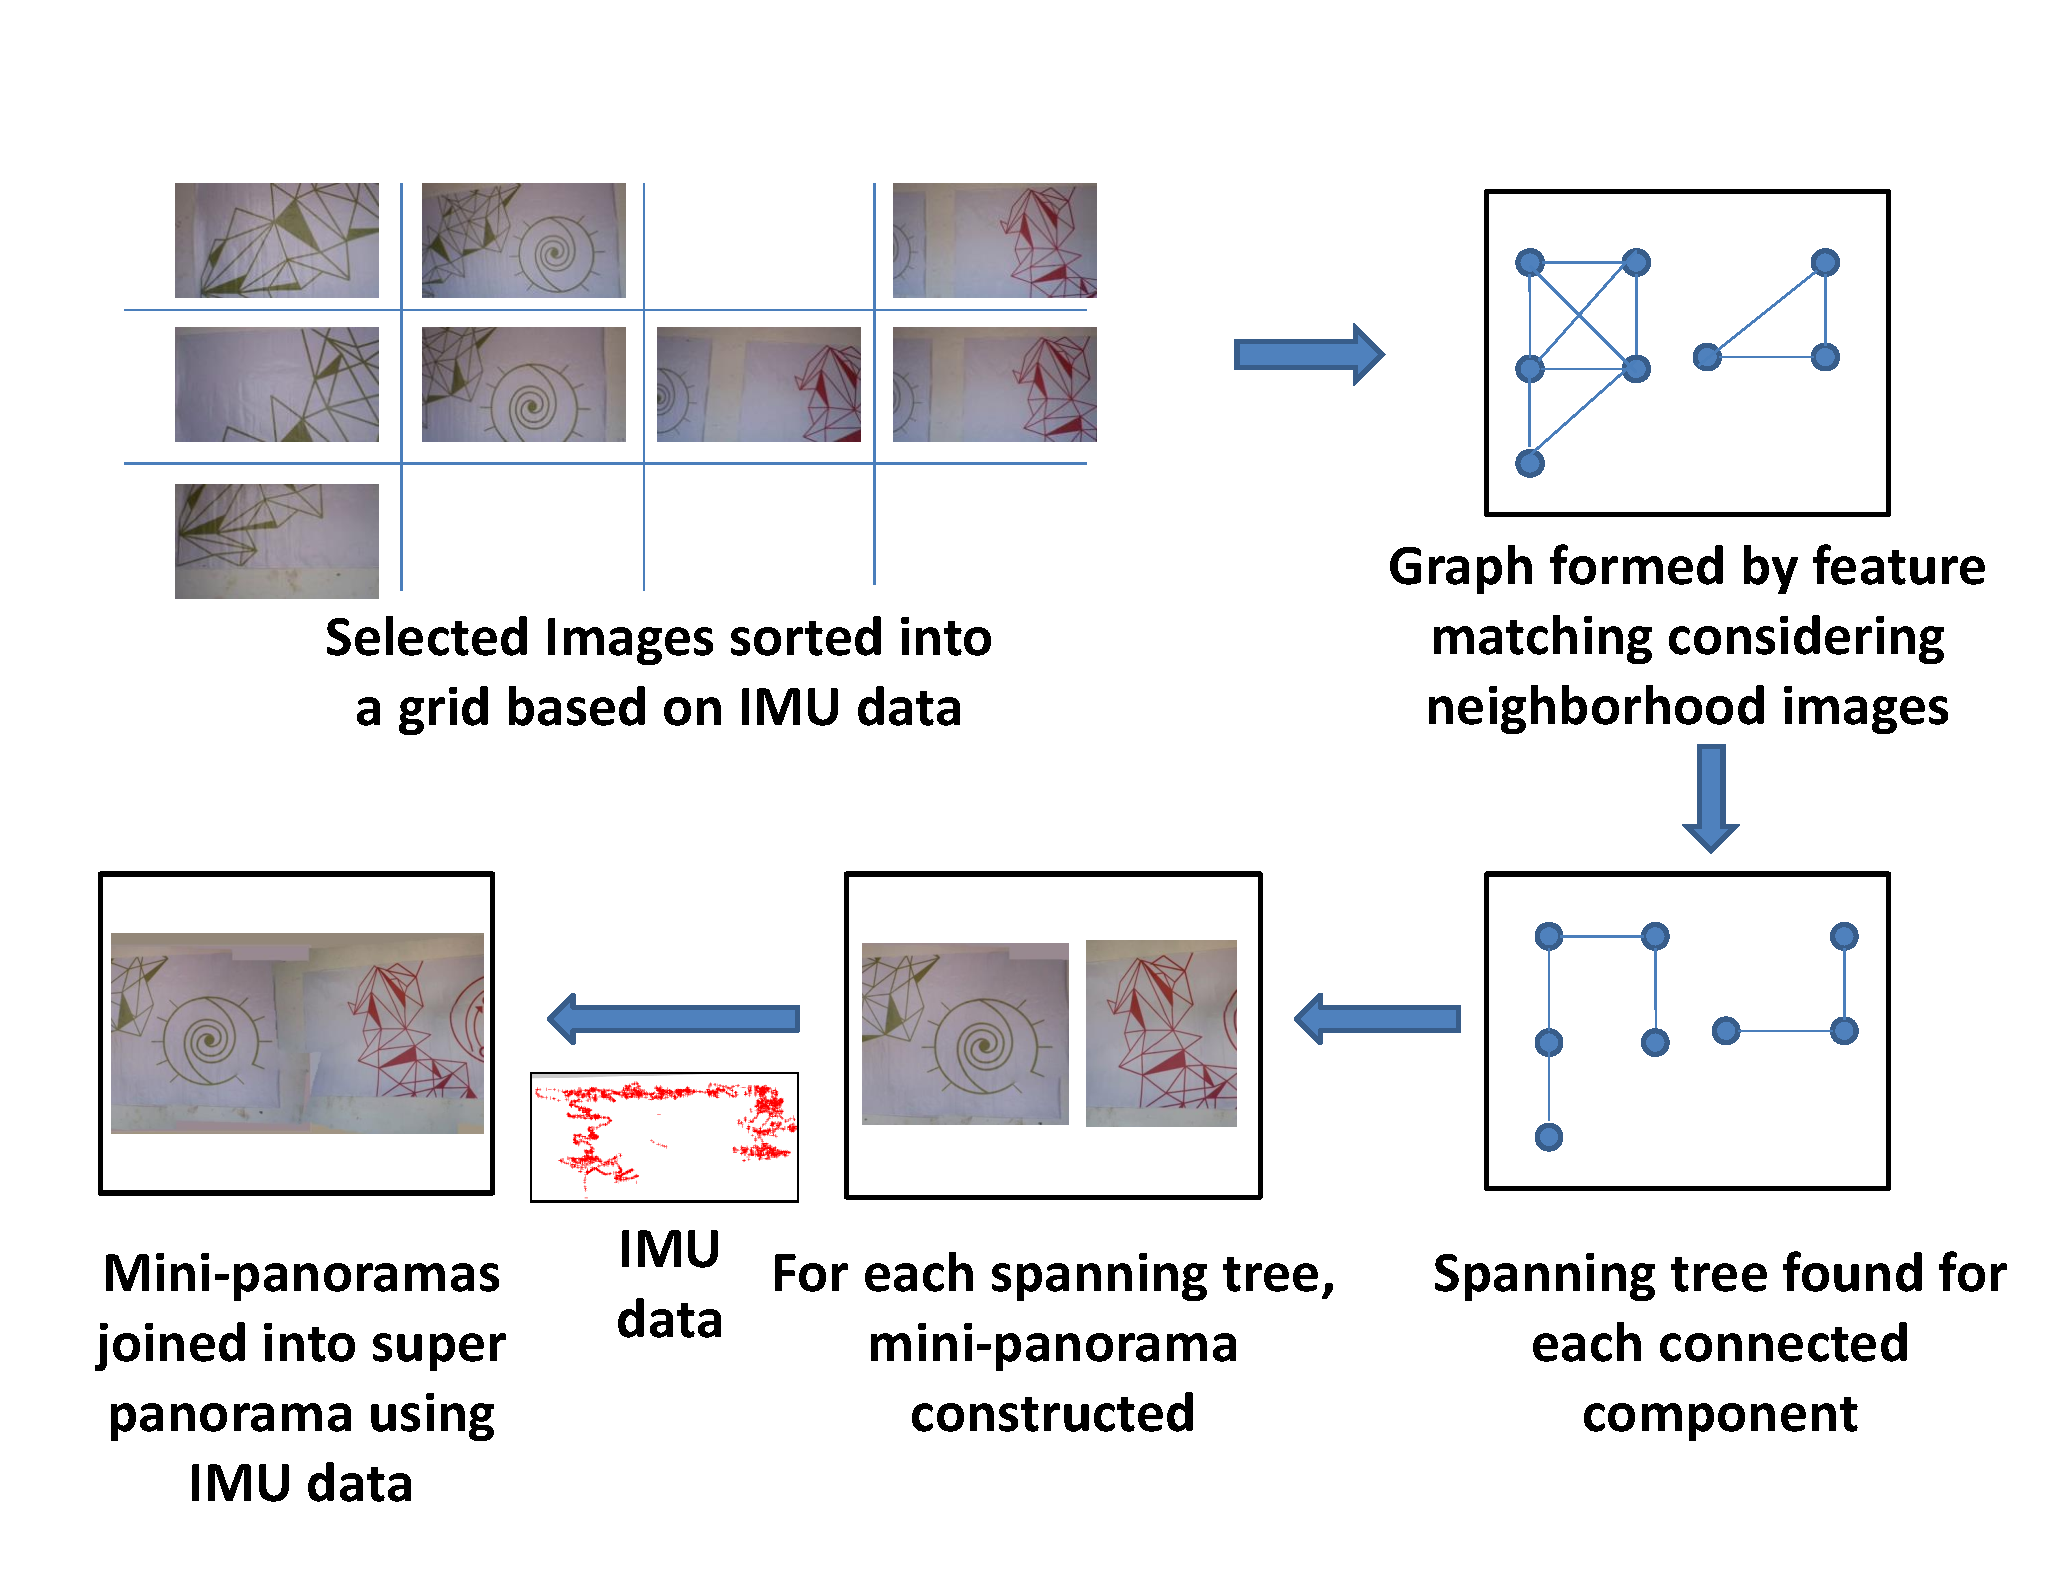
\includegraphics[width=\textwidth]{figures/vacantSpaces/graphCreation} 
  \caption[Creation of Mini-panoramas]{ \label{fig:graph} Interesting images
  acquired are segmented and individual (mini-panoramas) are constructed. These
    are then later combined into the desired super-panoramas using IMU data.}
\end{figure}    

\subsection{Super-panorama}
In this section, we consider the situation when programs like
AutoStitch fail.  We assume that the output of the previous step has
resulted in multiple spanning trees where each spanning tree center
corresponds to a specific depth. This is the depth of the center of
the spanning tree (estimated from the IMU data) since we have stitched all images by taking the
spanning tree center as a reference.  Individual panoramas for each
spanning tree termed mini-panoramas have been created. A
super-panorama must be created from mini-panoramas; these usually
correspond to different depths for at least two reasons.

First, it is invariably difficult, if not impossible, to control a
quadcopter to be at the exact depth even in indoor scenes.  The
aerodynamics and the thrust produced tends to make the quadcopter
drift.  Second, it might also be necessary to let the quadcopter probe
and come closer to the scene so as to get a ``good picture''.

A super-panorama is done using a two-step process. Assume two trees in
the forest corresponding to area A and area B of the scene (see
Figure~\ref{fig:stereo}). 
\begin{figure}[h!]
  \centering
  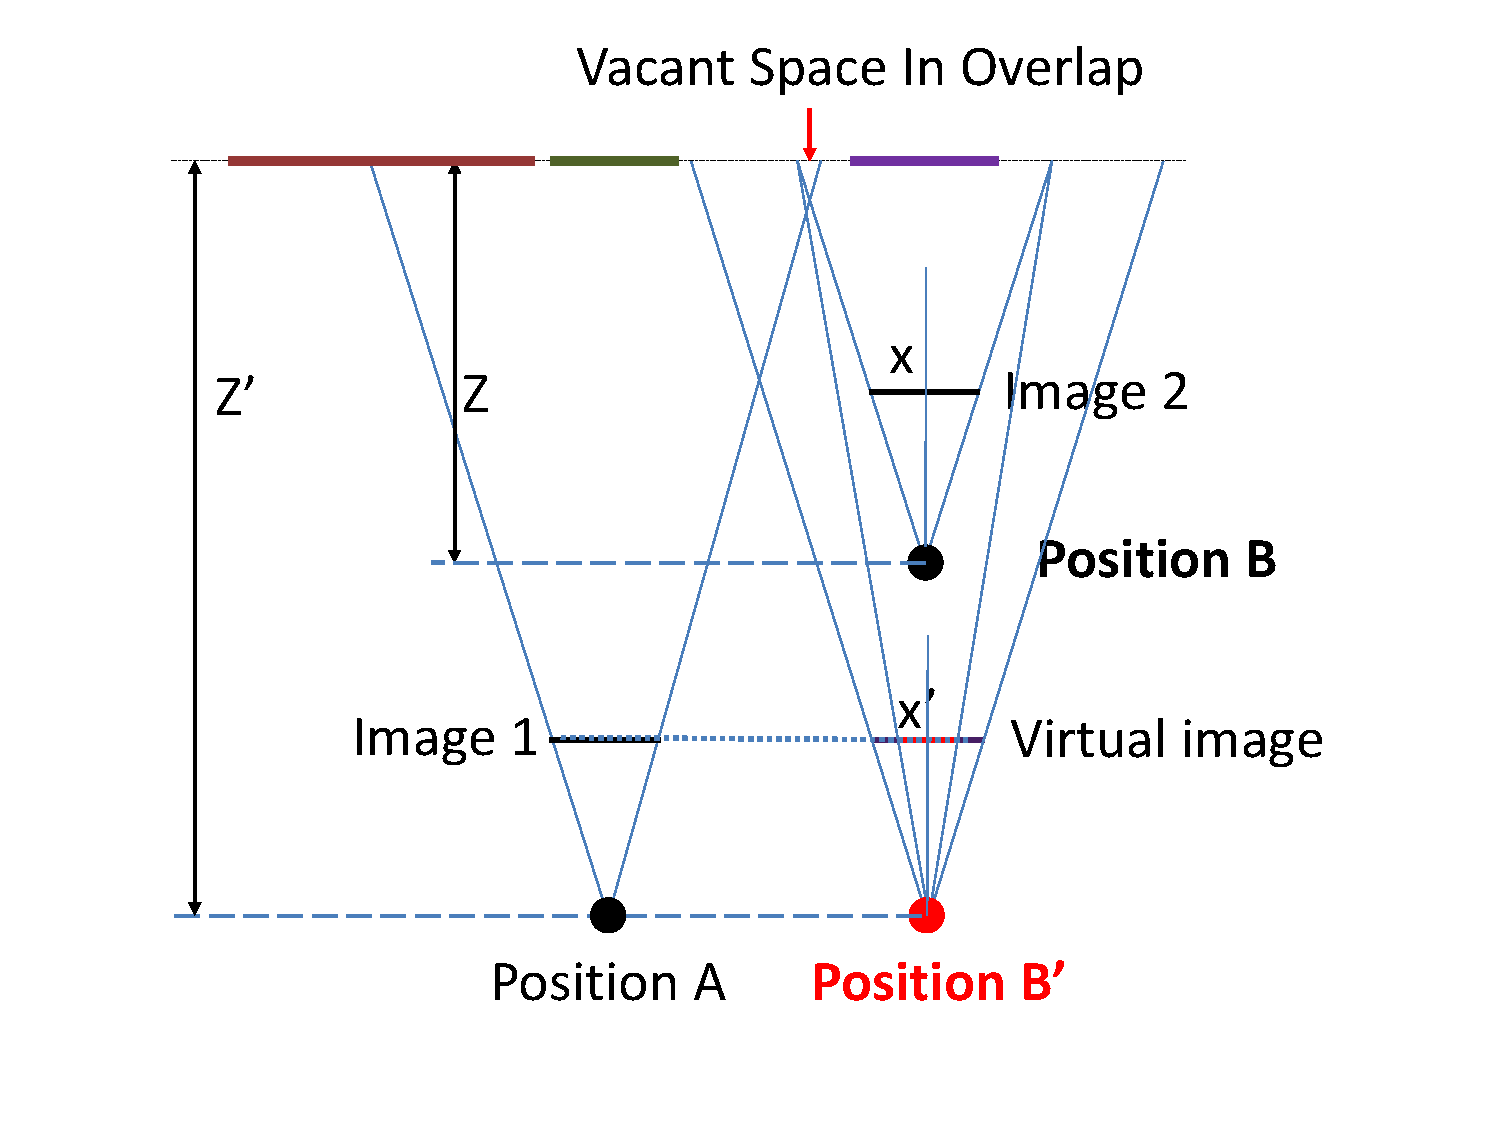
\includegraphics[width=0.8\textwidth]{figures/vacantSpaces/move} \\
  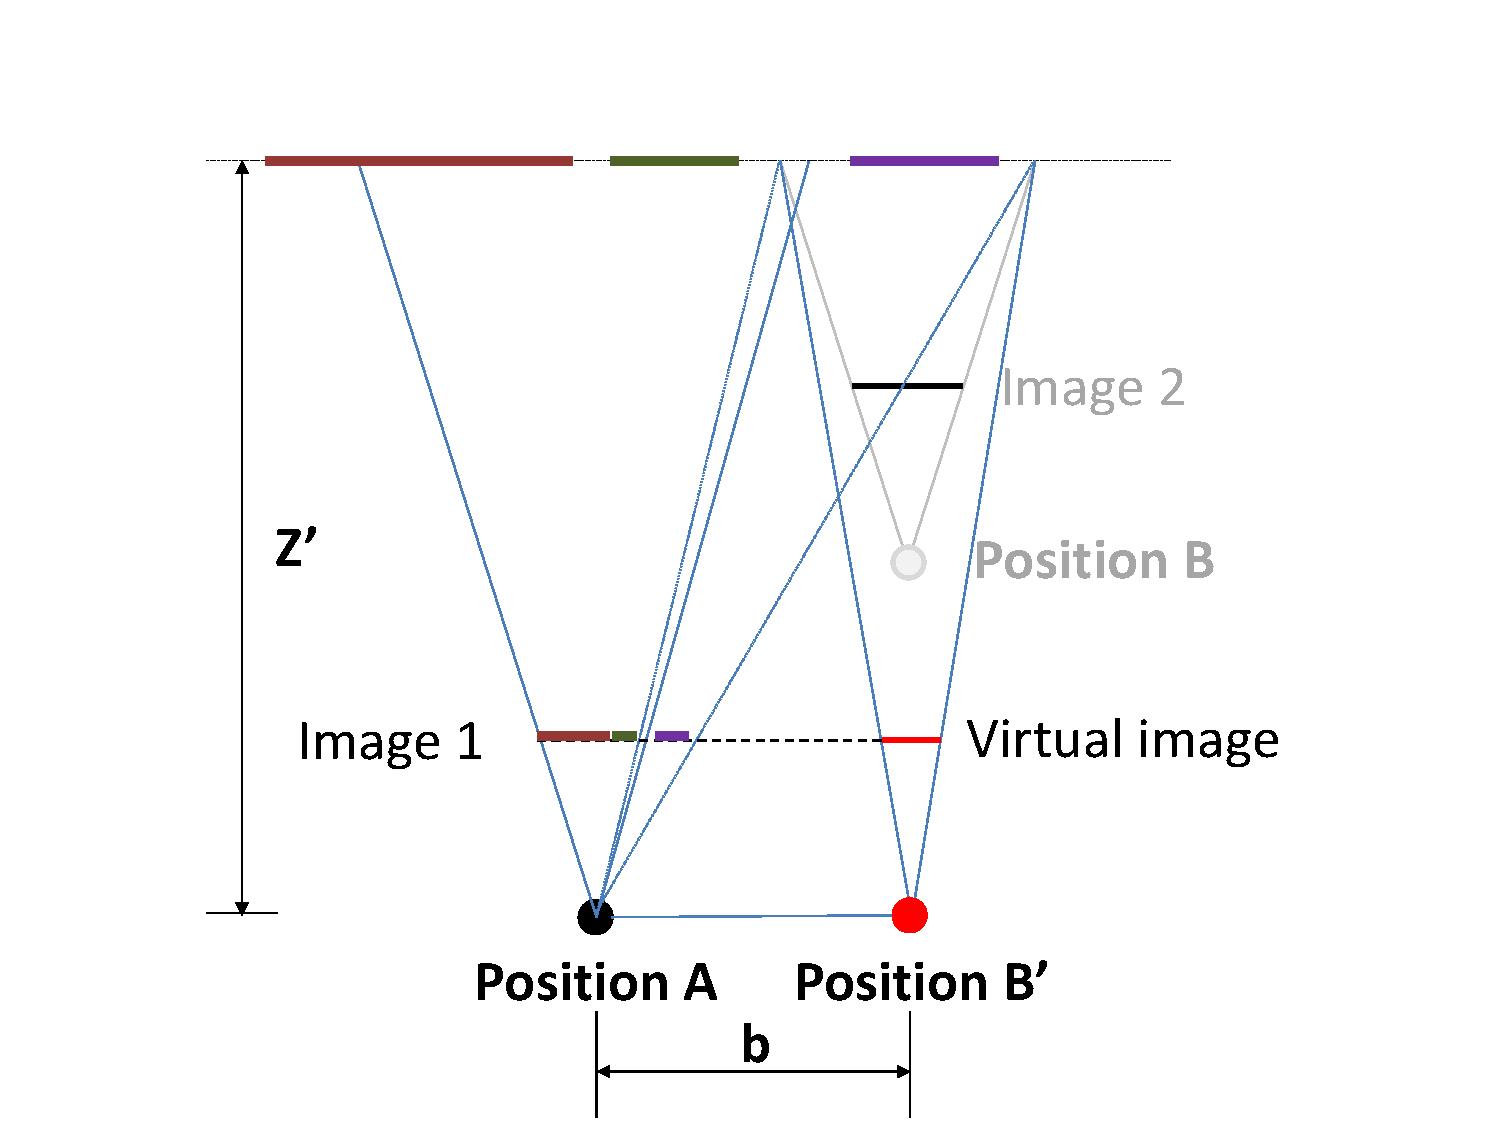
\includegraphics[width=0.8\textwidth]{figures/vacantSpaces/stereo} 
  \caption[Creation of Super-panoramas]{ \label{fig:stereo} (Top) The virtual
  picture as seen from position B' is computed using Equation~\ref{eq:moveRelation} from the real picture
    taken from B.  (Bottom) Using the stereo disparity, calculated from the baseline 
   width b and depth Z',  it is possible to depict the composite scene obtained from both A
  and B' (from the viewpoint of A).}
\end{figure}    
Assume that a mini-panorama is created from these two areas and the
depth of the planar surface from the camera is more for A, than for
B. We then take the mini-panorama image captured at B, and `move' it to
a new location B' whose depth (from the imaged surface) is the same as
that of A. The resulting image  will be smaller; the images are
related by the equation
\begin{equation}
  \label{eq:moveRelation}
  {\bf \frac{x'}{x} = \frac{Z}{Z'}}
\end{equation}
where {\bf x} (respectively {\bf x'}) represents a pixel location of
the image in B (respectively, B') and 
{\bf Z} (respectively {\bf Z'}) represents the depth of the images
surface from B (respectively, B').

In order to form a super-panorama from the depth of A, we can now
treat the resulting images from A (unchanged) and B’ (computed from
Equation~\ref{eq:moveRelation}) forming a simplistic stereo pair at
the depth of position A.  Using the stereo disparity formula we can
``place,'' from the viewpoint of A, the image captured from B',
thereby creating a super-panorama. (We could as well present the
entire scene from the viewpoint of B' (since it is at the same depth);
we prefer these pictures to the one that one may be created from the
depth of B.)

% In theory, one may for the super-panorama from viewpoint B, by first
% moving position A to the same depth as of position B. But in that
% case, virtual image of A formed at the depth of position A will be
% ``zoomed-in'' version which may cause pixelization.

\begin{figure}[h]
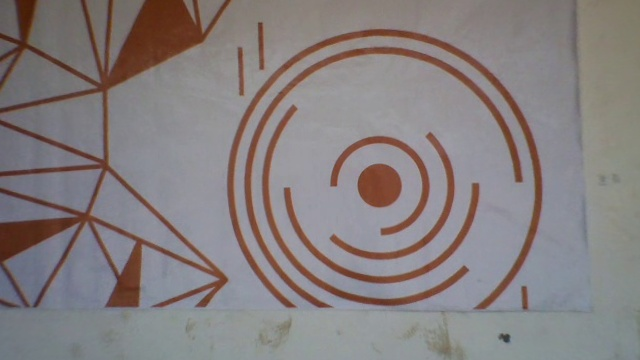
\includegraphics[width=0.48\textwidth]{images/left}

\includegraphics[width=0.48\textwidth]{images/right}
\caption[Example of super-panorama]{Candidate images for a super-panorama taken
from different depths. For context, see Figure~\ref{fig:results}.  These images are
  `reference' images (spanning  tree center) of individual  mini-panoramas.}
\label{fig:exmaple}
\end{figure}

\textbf{Example:} Consider two images (shown in Figure~\ref{fig:exmaple}) taken from the positions
(1.37, 0.85, 1.6), and (3.75, 0.98, 1.4).  As their depths are
different, we (virtually) move the second image by shrinking the
second image by a factor $\frac{1.4}{1.6}$, i.e., to 87\% of its
original size. With both images at the same depth (1.6m), the 
disparity of the second image is 
\begin{center}
$\text{disparity}_x = (3.75 - 1.37)f/1.6 = 839$\\
$\text{disparity}_y = (0.85 - 0.98)f/1.6 = -45$
\end{center}
where $f$ is focal length of the quadcopter camera in pixel units.

\subsection{Summary: Use of IMU}
The IMU data is used primarily for two purposes:
\begin{enumerate}
\item \textbf{Selection and ordering of images:} We use the IMU data
  to select representative images from the video and arrange them into
  rectangular grid according to the `spatial' neighborhood. It also
  disambiguates situations when multiple images that are spatially
  distant but have similar, repeated features.

\item \textbf{Super-panorama:} Whenever there are no features in
  the overlap region of two images, we use the IMU data to find the
  relative position of one image w.r.t. second image as shown in the
  example. 
\end{enumerate}
\setlength{\tabcolsep}{2pt}
\section{Experiments and Results}
\label{sec:results}

All our experiments have been completed with the inexpensive consumer
quadcopter called a Parrot's AR Drone 2.0. The imagery acquired were
from actual graffiti painted on large walls as well as posters in an
exhibition.  We have used the ROS-based ARDrone Autonomy
Driver to communicate with the drone. For the purpose of showing the
efficacy of our method, we also took a picture of the scene from a
distance with a smartphone camera to better understand the scene.

We have implemented our algorithm in C++ using the OpenCV library
(OpenCV 2.4.9). Experiments were performed on a PC with Intel Core i7
processor(@3.4GHz) and 8GB RAM.  
%The source code to produce
%interesting images from a video, and to generate the super-panorama,
%as well as the data sets used in this paper will be made publicly
%available after acceptance of the paper.

\subsection{Selecting Images}

In our first experiment, we wanted to ensure that the selection of
images done was comprehensive and useful.  We sent the drone to image 
an outdoor scene with no vacant space. This experiment was conducted
in an outdoor environment. We note here that there were approximately
3000 images in the raw video.  AutoStitch and Photoshop were unable to 
cope  when fed with this large number of frames.

One way to produce some sort of mosaic was to simply reduce the amount
of data given to AutoStitch.  Figure~\ref{fig:sac3}(a) shows uniformly
(time) sampled images from the video.  When these sampled images are
given to AutoStitch or to Adobe Photoshop, we find
(Figure~\ref{fig:sac3}(b)) that these programs are able to produce
some output, but the results are not satisfactory.

Instead of feeding time-sampled images, we ran our albumization
algorithm (as explained in Section~\ref{sec:selection}) on the video
which resulted in $N = 5$ images.  Though the number of input images
in the video is large, the total distance covered by the quadcopter in
this duration (of around 90 seconds) is small; thus the
number of distinct images returned by the algorithm shows a dramatic
reduction. Figure~\ref{fig:sac3}(c) shows examples of selected images.
Many of the images are similar to the time sampled version; however,
the occasional differences are enough to make AutoStitch work. The
results are shown in Figure~\ref{fig:sac3}(d).


\begin{figure}[hb!]
\centering
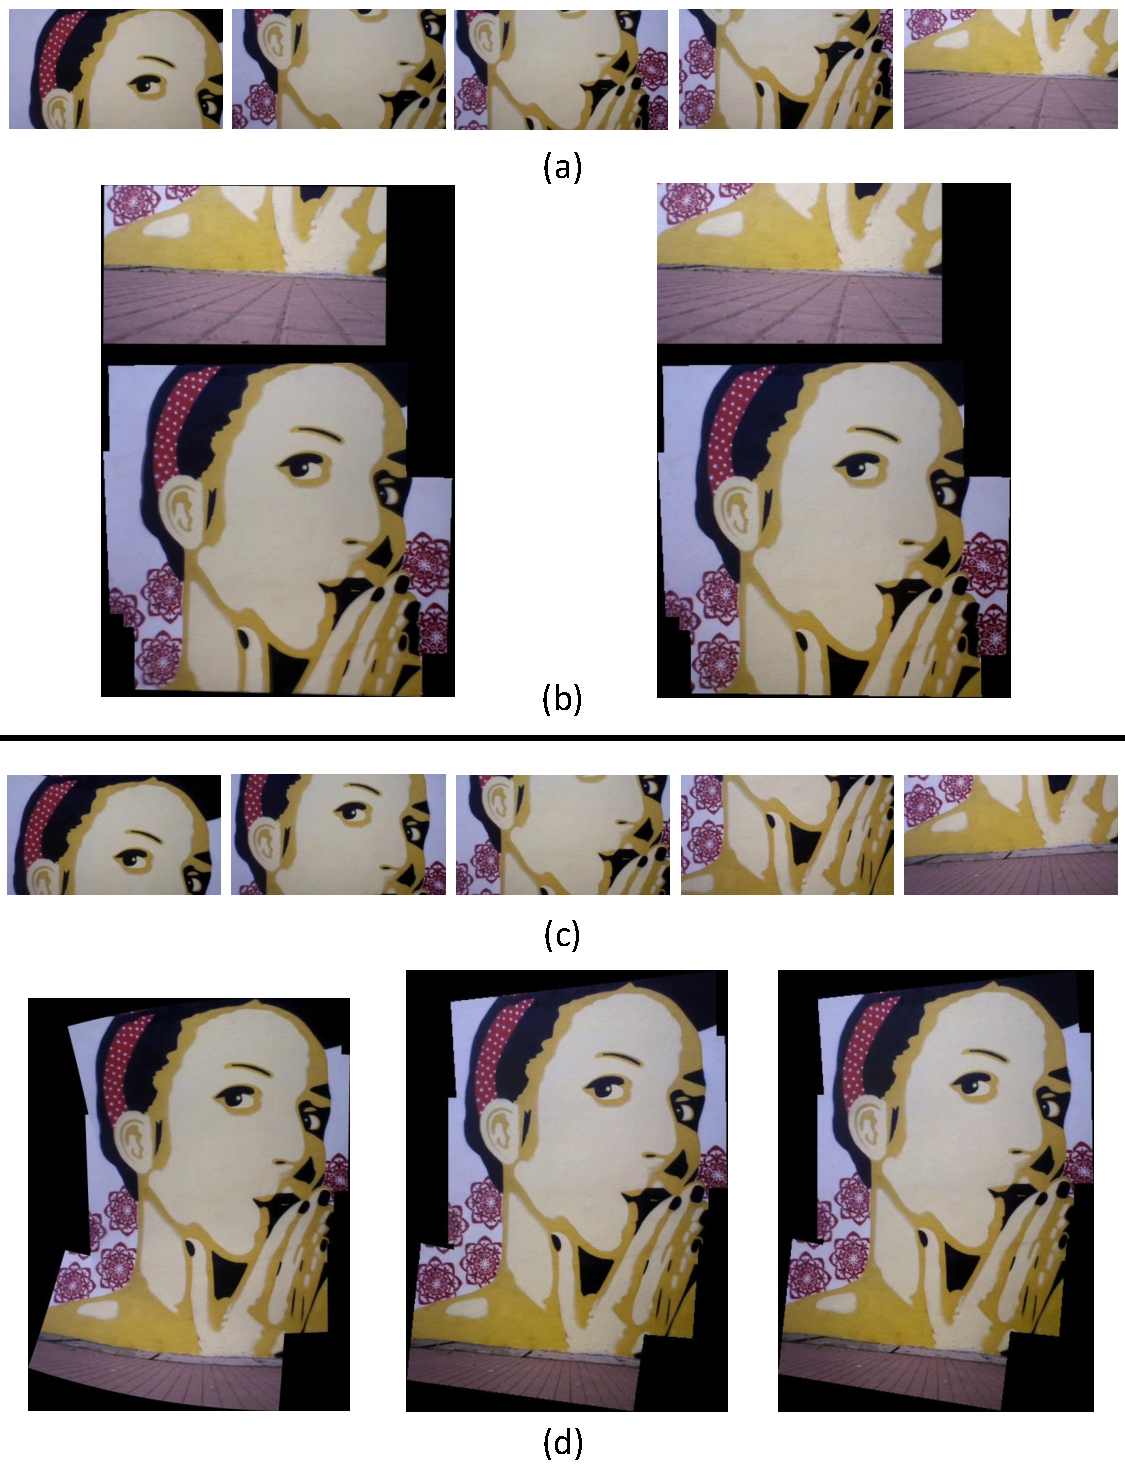
\includegraphics[width=0.87\linewidth]{figures/vacantSpaces/ValidationResult}
\caption[Validation Result: Lady]{ (a) Uniformly sampled images from an outdoor
video expedition.  (b) The output of the state of the art photo stitchers
  (left:AutoStitch, right:Adobe Photoshop CS6) on uniformly time
  sampled images.  As time sampled images do not guarantee coverage of
  the scene, the panorama is broken. The top portions do not belong at
  the right place (see (d)) (c) Salient image selection from the set of
  approximately 3000 images using positional information. (d) When
  salient images are given to AutoStitch (left) and Photoshop (middle),
  we can create a panoramic mosaic (since there are no vacant
  spaces). We also show the result from our stitching algorithm
  (bottom right).}
\label{fig:sac3}
\end{figure}

In summary, this experiment provides evidence to show that (a) our
albumization algorithm is reasonable and (b) our stitching
results are comparable to that of AutoStitch for the kind of scenes
considered.

\subsection{Indoor Imagery with Vacant Spaces}

Our next selection of experiments was conducted in an indoor
environment.  

The input stream had about 4300
images. The selection algorithm (Section~\ref{sec:selection}) pruned the video
into $N=5$ images. A sample of the selected images are seen in Figure~\ref{fig:vacantTeaser}.

There were two disconnected components in the resulting graph.
AutoStitch was unable to produce any reasonable output as seen in
Figure~\ref{fig:vacantTeaser}.  The scene, captured from a distance is also
shown.  One can see a better orthographic view of the posters.

\textbf{Cars:}
In an another experiment, the input stream had about 9000 input
images.  The selection algorithm (Section~\ref{sec:selection}) pruned
the video into $N=13$ images. A sample of the selected images are seen
in Figure~\ref{fig:indoor_results}(a).  The scene as captured by a
smartphone can also be seen, as well as the outputs of the state of
the art stitchers. Note that AutoStitch is only able to stitch the
upper half of the scene.  Our result
Figure~\ref{fig:indoor_results}(e) clearly stands out in comparison.

\begin{figure}
\centering
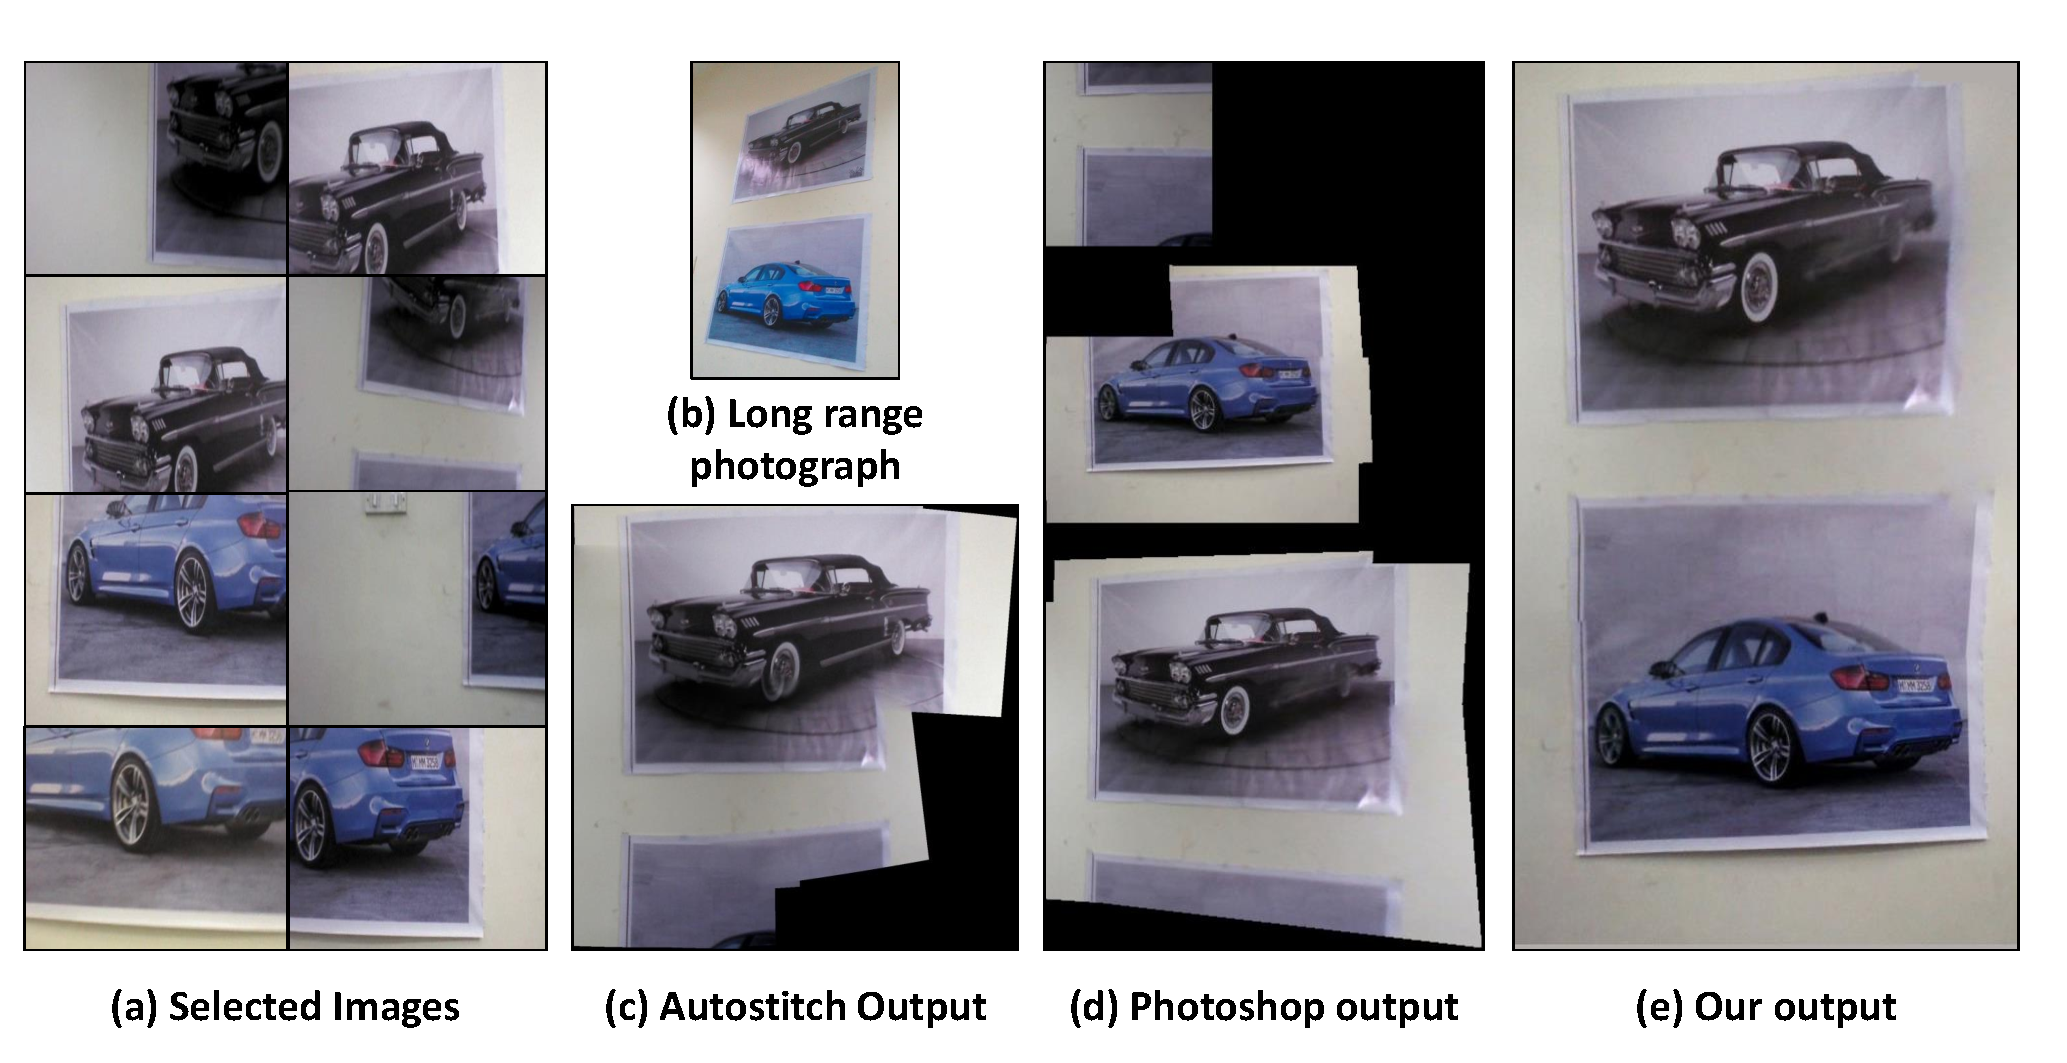
\includegraphics[width=\linewidth]{figures/vacantSpaces/indoor_results}
\caption[Result: Cars]{ (a) Pruned images from the quadcopter video using our
  saliency algorithm of (b) an indoor scene. This long range photograph
  has been captured separately by a smartphone camera only for
  context. Notice a significant vacant space in the imagery.  (c)
  The output of AutoStitch -- only the upper half of the scene is output.
  (d) The output of Adobe Photoshop CS6 -- the vacant space posed a problem to the
  feature matching algorithm, so instead of a mosaic, individual
  pieces were output as mini-panoramas (e) Our output on the selected
  images. We are able to present the scene in high fidelity in an
  orthographic view.}
\label{fig:indoor_results}
\end{figure}

\textbf{Aircrafts 1:} The input stream had about 9100 images. The selection
algorithm pruned the video into $N=14$ images. The scene as captured by a
smartphone can also be seen in Figure~\ref{fig:aircrafts1}(b). A sample of the
selected images is seen in Figure~\ref{fig:aircrafts1}(a).
Figure~\ref{fig:aircrafts1}(c,d,e) shows the comparison of outputs of state of
the art stitchers with the output of our algorithm. As there are vacant spaces,
AutoStitch~\cite{autostitch} is able to join only top part of the scene, while
Photoshop~\cite{photoshop} is showing two disconnected components.
In contrast, since we use positional data, our output is an acceptable mosaic,
and shows an orthographic view.

\begin{figure*}[h!]
	\centering
	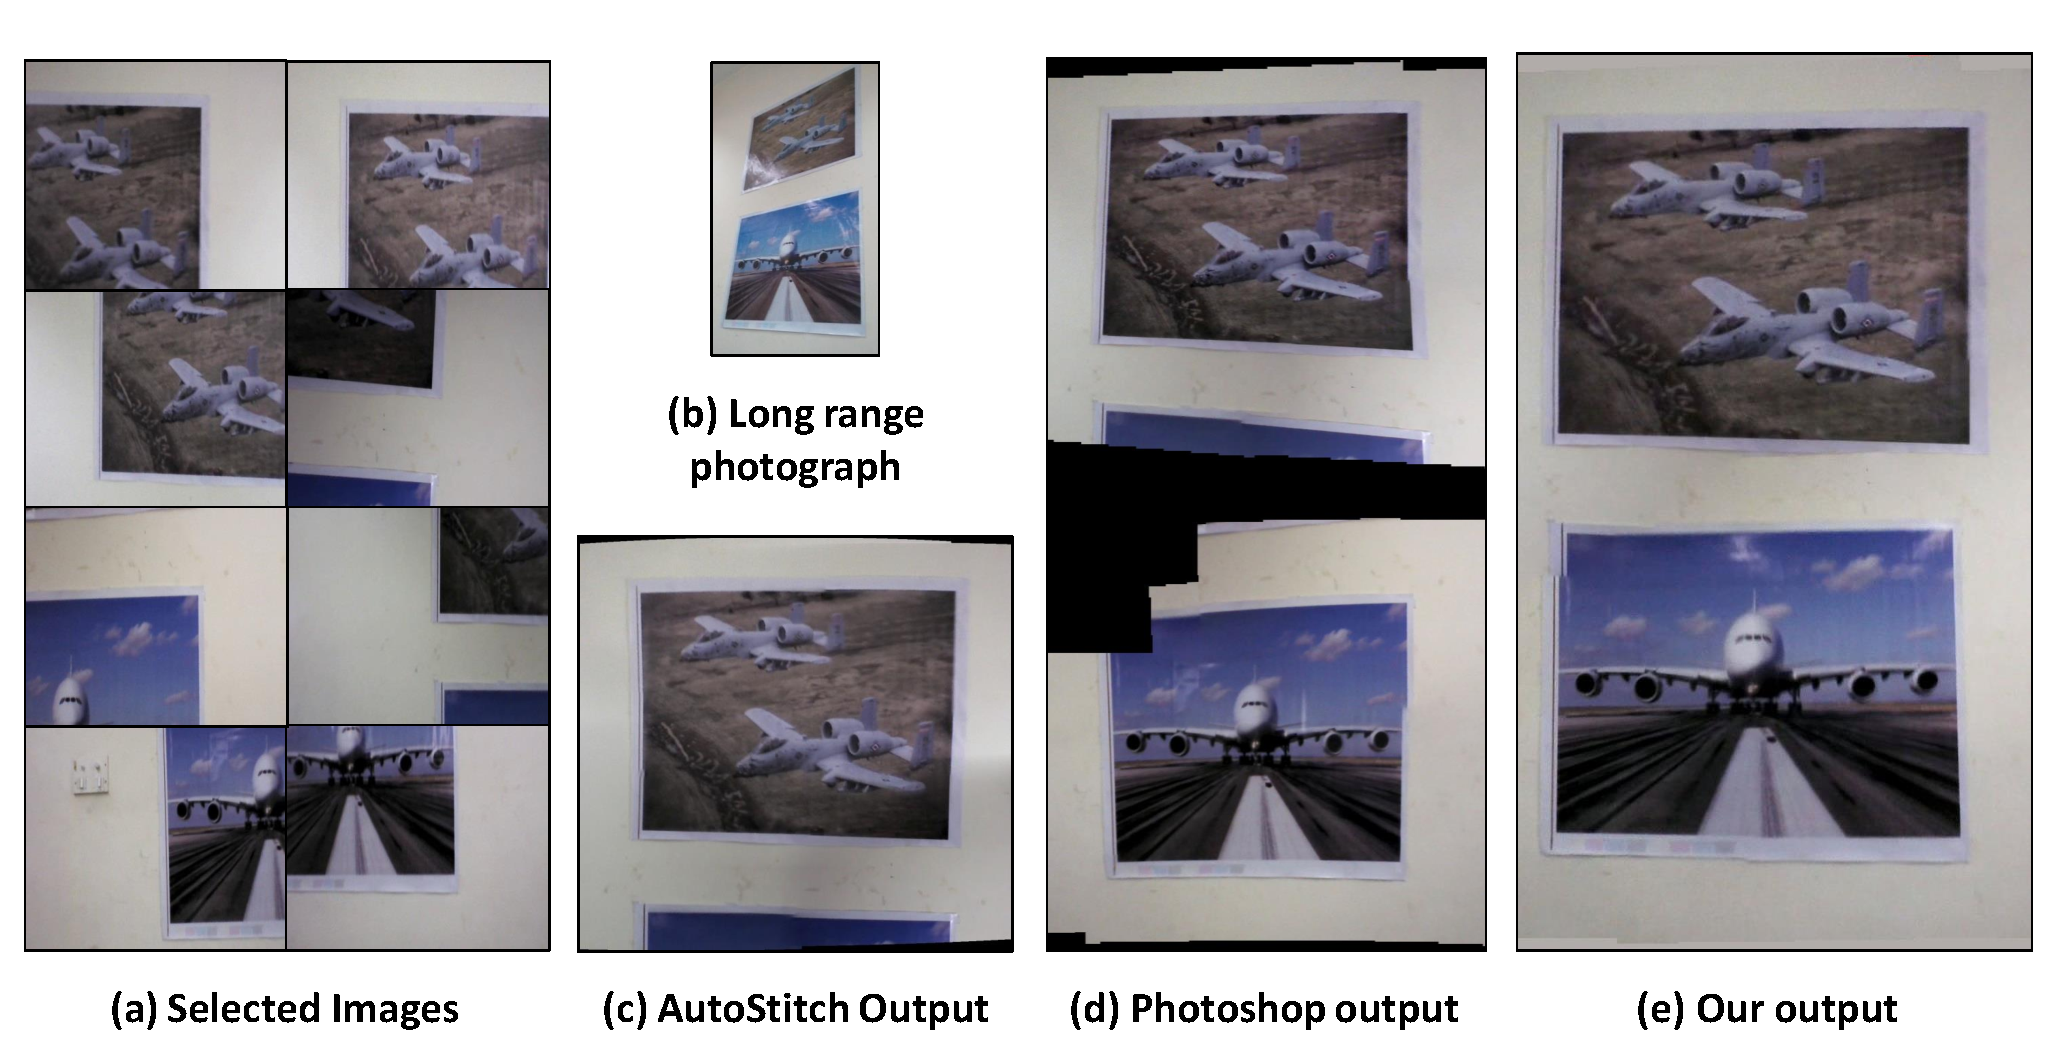
\includegraphics[width=\linewidth]{figures/vacantSpaces/aircrafts1}
	\caption[Result: Aircrafts]{(a) Pruned images from the quadcopter video using
	our saliency algorithm of (b) an indoor scene. This long range photograph has been captured separately by a smartphone camera only for context. Notice a significant vacant
space in the imagery. (c) The output of AutoStitch - only the upper half of the scene is output. (d) The output of Adobe Photoshop CS6 - 
the vacant space posed a problem to the feature matching algorithm, so instead of a mosaic, individual pieces were output as mini-panoramas (e) Our output on the
selected images. We are able to present the scene in high fidelity in an orthographic view.}
	\label{fig:aircrafts1}
\end{figure*}

\subsection{Outdoor Imagery with Vacant Spaces}

\begin{figure}[h!]
\centering
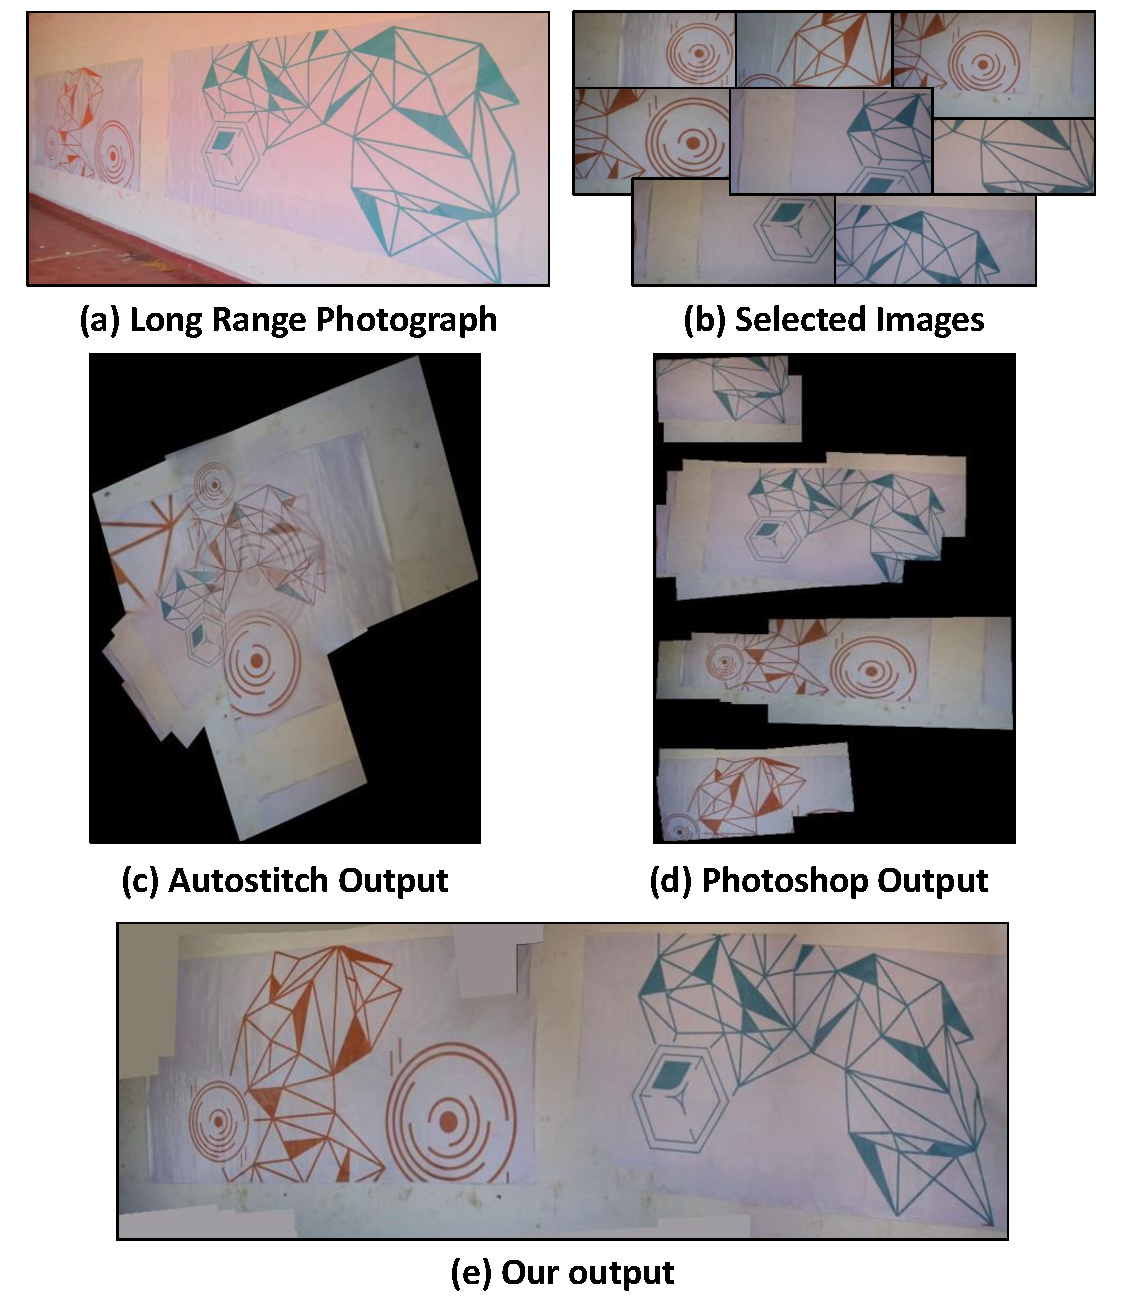
\includegraphics[width=\linewidth]{figures/vacantSpaces/orange_blue}
\caption[Result: Outdoor Exhibition]{(a) An outdoor scene captured by a standard
camera in an exhibition. The approach to the area is normally cordoned off and one
  needs permission to get a quadcopter to take the picture.  Notice a
  significant gap between the two posters.  (b) Pruned images from the
  quadcopter video using our saliency algorithm. (c) The output of
  AutoStitch on the selected images. The mosaic is not reasonable
  presumably because of the confusion in features. (d) The output of Adobe
  Photoshop CS6 on the selected images. The vacant space posed a
  problem to the feature matching algorithm, so instead of a mosaic,
  individual pieces were output as mini-panoramas (e) Our output on
  the selected images. We are able to join two posters (separated by
  vacant space) using the IMU data.}
\label{fig:results}
\end{figure}

Our next set of experiments were conducted in an outdoor
environment. The input stream had about 12000 images. The selection
algorithm pruned the video into $N=30$ images. A sample of the
selected images are seen in Figure~\ref{fig:results}(a).  The scene as
captured by a smartphone can be seen in Figure~\ref{fig:results}(b).
Figures~\ref{fig:results}(c), (d) and (e) shows the comparison of outputs of
state of the art stitchers with the output of our algorithm. Note that
AutoStitch is getting confused by too many matching features. 
Please see supplementary material for results on other indoor as well as outdoor datasets.

Figure \ref{fig:results2} shows comparison of outputs of state of the art
stitchers with the output of our algorithm on another dataset.

\begin{figure}[h!]
\centering
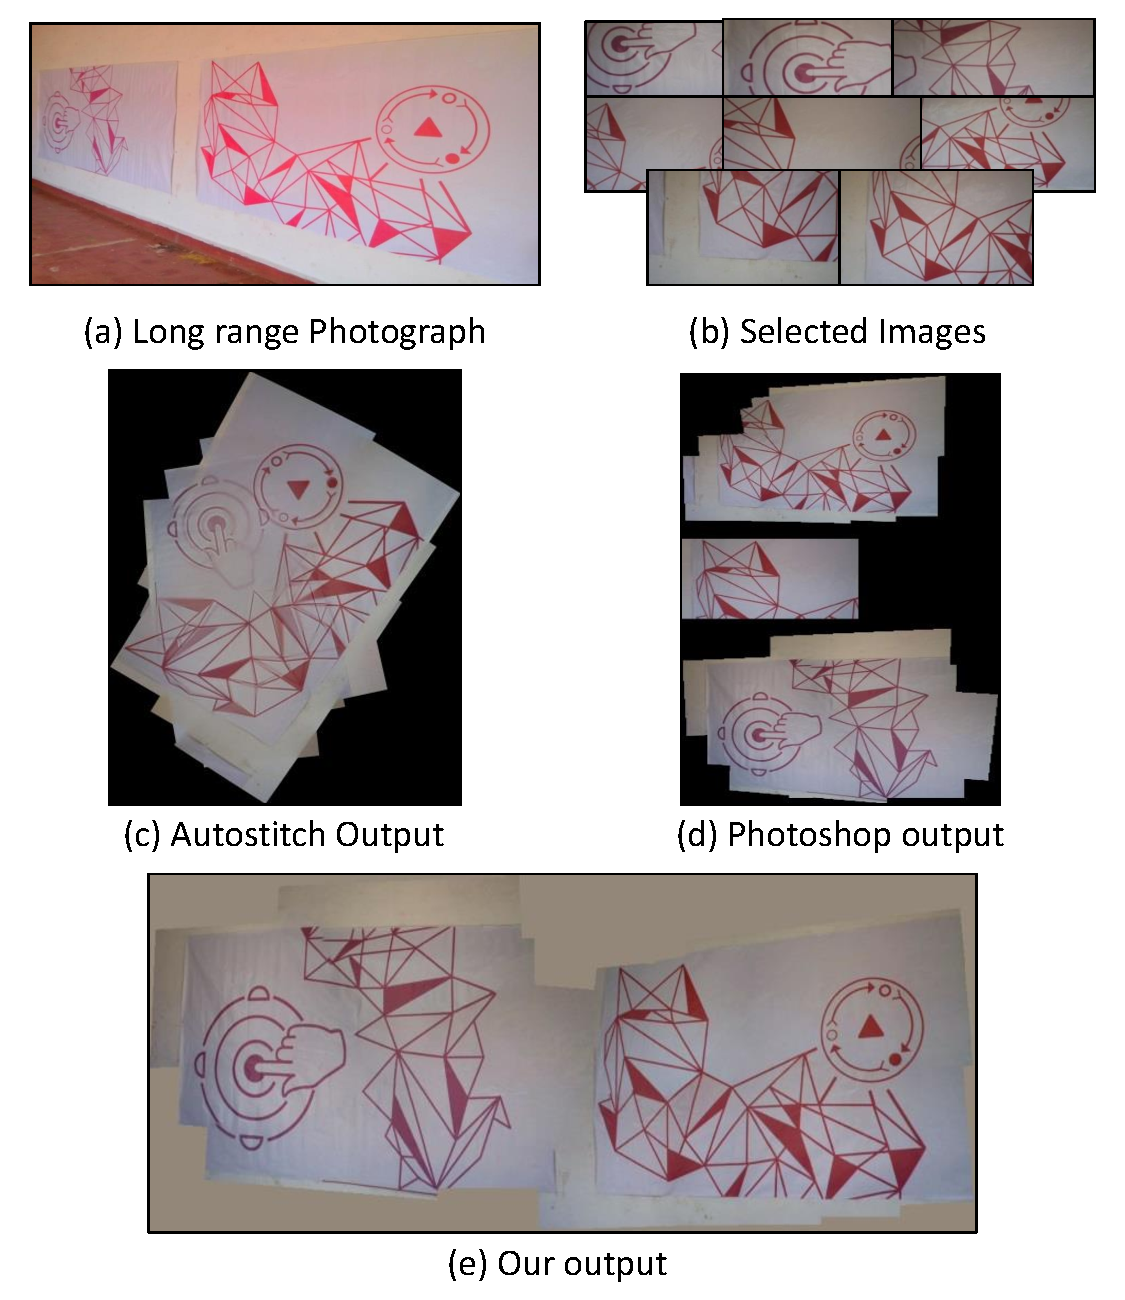
\includegraphics[width=\linewidth]{figures/vacantSpaces/Purple_red} 
\caption[Result: Outdoor
Exhibition 2]{(a) Another outdoor
scene captured by a standard camera in an exhibition. The approach to the area is normally cordoned off and one
  needs permission to get a quadcopter to take the picture.  Notice a
  significant gap between the two posters.  (b) Pruned images from the
  quadcopter video using our saliency algorithm. (c) The output of
  AutoStitch on the selected images. The mosaic is not reasonable
  presumably because of the confusion in features. (d) The output of Adobe
  Photoshop CS6 on the selected images. The vacant space posed a
  problem to the feature matching algorithm, so instead of a mosaic,
  individual pieces were output as mini-panoramas (e) Our output on
  the selected images. We are able to join two posters (separated by
  vacant space) using IMU data.}
\label{fig:results2}
\end{figure}


\subsection{Analysis}

The performance of our algorithm as a function of the scene, as well
comparison with other software is summarized in
Table~\ref{tbl:results}.  It can be seen that, whenever there is
vacant space between adjacent images, AutoStitch produces only
one component, presumably the largest.  Adobe Photoshop outputs all disconnected
components. Sometimes due to the lack of spatial proximity
information, the resulting images (or components) are disconnected instead of being 
mosaiced (unlike AutoStitch). In contrast, in all cases, our algorithm
successfully uses proximity information which results in a reduced number of mini-panoramas. 

As expected the number of selected images in our saliency algorithm
varies based on environment considerations (outdoor/indoor), the
average depth from the scene, and the total scene area.
 
\begin{table*}
\scriptsize

\newcolumntype{C}{ >{\centering\arraybackslash} m{1.1cm} }
\newcolumntype{D}{ >{\centering\arraybackslash} m{1.5cm} }

\begin{tabular}{|C|C|C|C|D|D|D|m{6.5cm}|}
\hline
Dataset 
& Number of Images in video 
& Approx. planar area covered
& Number of selected images 
& AutoStitch: \# Components 
& Photoshop: \# Components
& Our algorithm: \#mini- panoramas
& \multicolumn{1}{p{6.5cm}|}{\centering Remarks}\\
\hline

\hyperref[fig:sac3]{Lady} & 3000 & 60 sqft. & 5 & 1 & 1 & 1 & As there are enough features
in the intersection of selected images, AutoStitch, Photoshop as well
as our algorithm produces the  panorama correctly.\\\hline
%Spray Woman} & 9000 & 70 sqft. & 15 & 1 &
%1 & 1 & As there are enough features in the intersection of selected images,
%AutoStitch, Photoshop as well as our algorithm gives full panorama
%correctly. As this scene was captured nearer from the plane than
%earlier, we need to select more images than earlier dataset.\\\hline 

\hyperref[fig:vacantTeaser]{Indoor exhibition} & 4300 & 40 sqft. & 5 &
1 & 2 & 2 & As there is vacant space between the two posters,
AutoStitch produces only one panoramic image. Photoshop outputs two
posters as two disconnected components; these correspond to our mini-panoramas.
\\\hline 

\hyperref[fig:indoor_results]{Cars} & 9000 & 60 sqft. & 13 & 1 & 3 & 3 &
As there is vacant space between the two visuals, AutoStitch produces
only one panoramic image, the black vehicle.  In the case of
Photoshop, two of the three disconnected 
components represents two partial visuals, while the third component is
the intersection  between the two cars -- this portion contains featureless
space.\\\hline

\hyperref[fig:results]{Outdoor exhibition} & 12000 & 80 sqft. &
30 & 1 & 4 & 2 &  AutoStitch is confused by the replicated features in
the two posters which are sometimes proximal and sometimes
geographically distant.  A single panorama is produced, but the output
is incorrect. We use the IMU data
for arranging the images in a spatial neighborhood; we have fewer
mini-panoramas.  Photoshop is not able to produce a super-panorama and
the number of disconnected components in Photoshop's output is larger
than the number of mini-panoramas.\\\hline  
\end{tabular}
\caption{Quantitative summary of  results}
\label{tbl:results}
\end{table*}



\section{Concluding remarks}

In this chapter, we have described a method of imaging large scenes
using a quadcopter enabling close orthographic views. We also defined
a new problem, that of computing a mosaic of a planar scene with
vacant spaces.  Vacant space relates to images in an input stream
where there are not enough features for traditional mosaicing
algorithms to estimate geometric warps to align the images.

Our solution to this problem is to use a quadcopter which
is capable of taking pictures.  The quadcopter has an inertial
measurement unit that is capable of outputting approximate
positions. Using this positional information, our algorithm selects an
``interesting'' subset of the video imagery.  This subset consists of
pictures taken with a moving camera; we reduce the resulting
problem of computing a mosaic to the stereo problem.  Our
method works on both indoor and outdoor scenes.

Controlling a consumer-focused inexpensive quadcopter can be
problematic; for instance, the quadcopter could have severe yaw and
roll.  We need a robust algorithm for autonomous navigation of quadcopter.
We will discuss vision based algorithms to control such quadcopters autonomously
in next chapter. We extend our work of mosaicing scene on a single planar
surface to scene spread over multiple planar surfaces.

\chapter[Multiplanar Imaging]{Autonomous Imaging of Multiplanar Regions through
Quadcopter}
\label{ch:multiplanar}
\section{Introduction}
Consider a visit to an art gallery or ancient temples. In such scenarios, we
would like to get an unrolled view of scenes depicted on the walls so that we
get the output mosaic of the input scene as if it is present on a single plane.
We have to capture each surface orthographically from close range to get minute
details. We may consider using Single-Lens Reflex (SLR) cameras or even
smartphones which are easily available for imaging such scenes. Many of these
cameras also have special modes to capture panoramas.
\begin{figure}[h!]
\centering
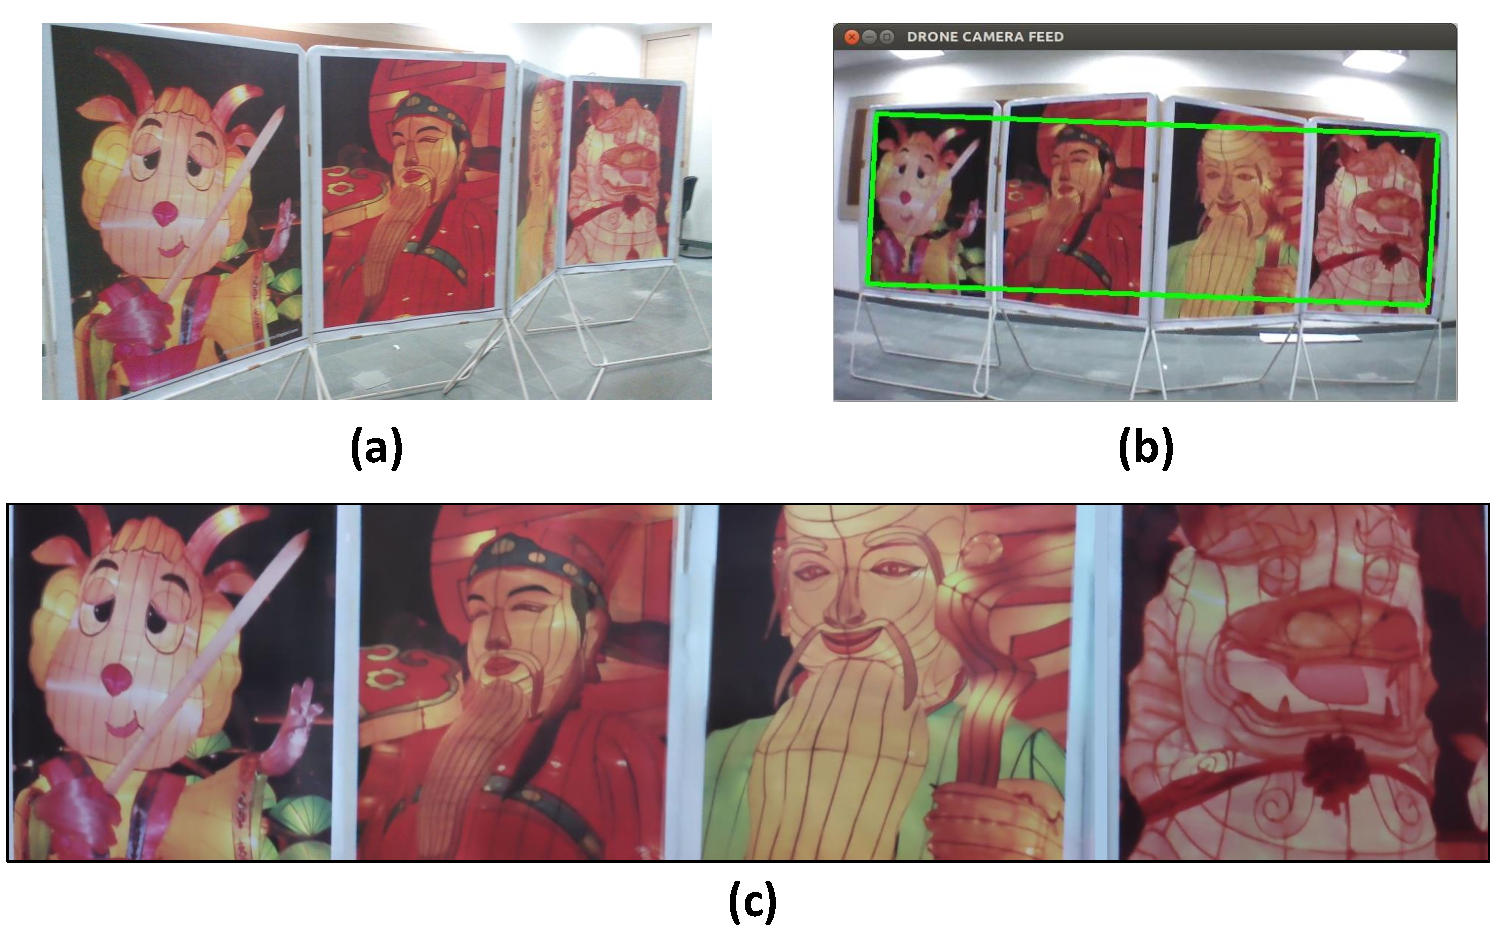
\includegraphics[width=0.98\linewidth]{figures/multiplanar/teaser2}
\caption[Overview of multiplanar imaging]{The multiplanar scene to be mosaiced is shown in (a). The long-range
photograph doesn't provide sufficient details of all the objects in the scene. A
quadcopter is maneuvered to allow a user to select the area of interest as shown
in (b). The final mosaicing output from this paper is shown in (c). The size of
our output is 3427 x 863 pixels.}
\label{fig:teaser}
\end{figure} 

\begin{figure}[htb]
\centering
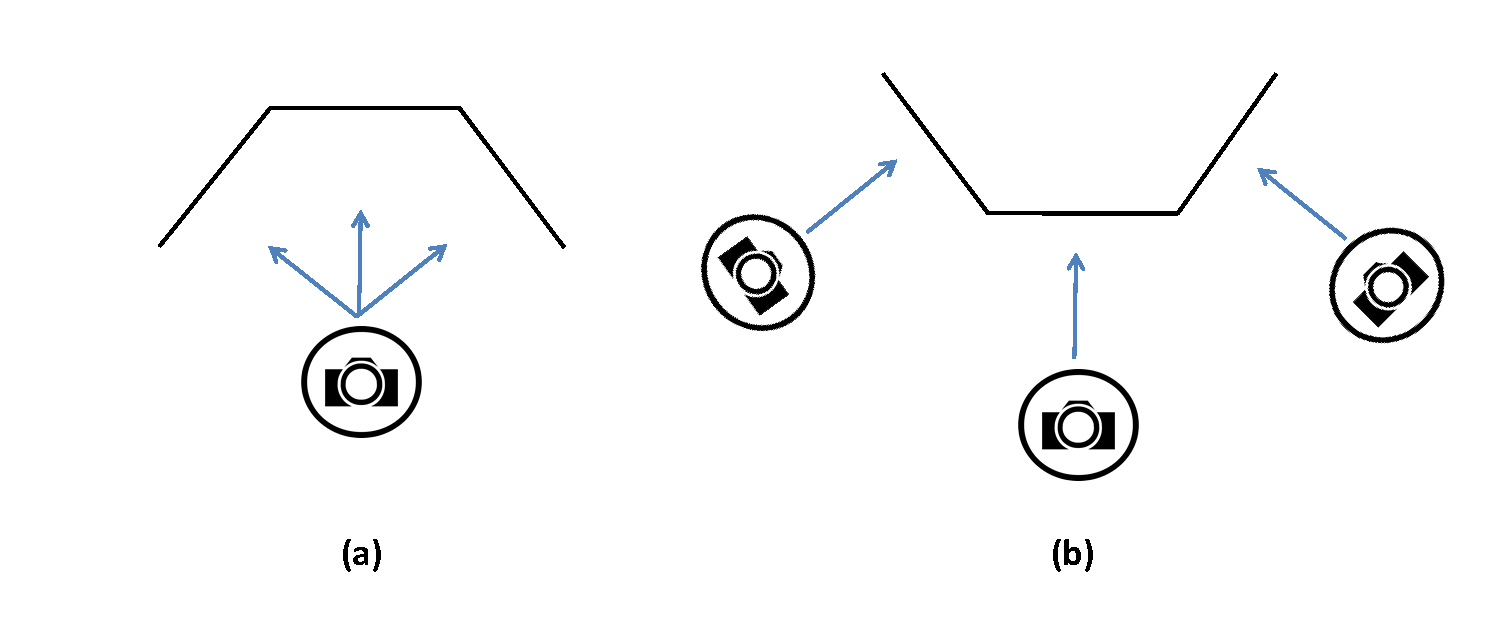
\includegraphics[width=\textwidth]{figures/multiplanar/ConcaveConvex}
\caption[Imaging concave surfaces versus convex surfaces ]{(a) Imaging concave surfaces. We do not
have to change our position, changing orientation is sufficient to capture the
whole surface. (b) While imaging a convex surface, one have to change the
position as well as the viewing angle. It makes the process
of building homography based panorama  theoretically impossible.}
\label{fig:convex_concave}
\end{figure}

However, in practice, when we use such cameras for capturing
panoramas, we do not get the close-up orthographic view of the scenes which are
present at a height or inaccessible to human. We also require a steady hand for
a long time while capturing panoramas which might be too tiring.

The limitation of cameras is that it can create a panorama with an orthographic
view, if the surface to be imaged is present on a single plane. We can also get
a panorama with an orthographic view, if the surface is concave and the camera
is kept at the center of the surface, as shown in 
Figure~\ref{fig:convex_concave}(a). However, if the surface (or part of it) is
convex,  as shown in Figure \ref{fig:convex_concave}(b), viewpoint (along with
the orientation) has to be changed while imaging. It prohibits the use of
panorama mode of most cameras. If any camera allows such panorama creation, the
output is distorted due to change in homography.

In scenarios where handheld devices cannot capture an orthographic view of a
large input scene, an inexpensive flying device such as a quadcopter can be
used. A quadcopter can cover any large scene with an orthographic view with
fine details (e.g., facial features of a person in Figure \ref{fig:teaser})
by flying in front of each part of the scene. However, manually controlling a
quadcopter to image a large multiplanar scene is a tedious task and hence
requires automation.

\textbf{Problem Definition}
Prasad et al.~\cite{Prasad16} have developed an imaging application with the use
of a quadcopter. It handles large scenes and scenes with featureless (vacant)
spaces.
%But a few things were not considered in \cite{Prasad16}.%
%The first one is regarding navigation and control of quadcopter.%
In \cite{Prasad16}, we have to manually navigate the quadcopter smoothly to
image large scenes from a close distance. There are various options available for manual
navigation and control of quadcopter. FPV (First Person View) controllers are
often used for controlling quadcopters. However, we have to do a lot of manual
adjustments while using FPV. Hence, if we have to capture large surfaces from a
specific depth, it would be very tiring. Also, it is not ensured that the
surface is imaged orthographically. There is a high probability of collision
between quadcopter and the imaging surface during these adjustments. 

Also in \cite{Prasad16}, the mosaicing algorithm could mosaic only if the scene
lies on a single planar surface. However, the real world is made-up of
multiplanar as well as curved surfaces. In fact, we have many circumstances where the input
scene is spread over multiple planes. In such cases, we would like to image each
planar region orthographically and then \textit{unroll} the whole scene by
joining the individual mosaics so that we get the output mosaic of the input scene as if it
is present on a single plane.
 
\textbf{Challenges}
We would like to autonomously navigate quadcopter to capture the whole scene.
Generally Global Positioning System (GPS) is used for navigation of UAVs. However, GPS
does not work effectively and precisely in indoor scenarios. Even in outdoor
scenario, we may not rely fully on GPS due to GPS jammer, spurious
signal, etc.. Hence, we require a reliable navigation system to maneuver the
quadcopter in an unknown environment.

A quadcopter has onboard an IMU (Inertial Measurement Unit)  which consists of
accelerometers, gyroscopes, and magnetometers. The IMU provides pose which can be
used to determine desired locations from where the whole scene can be covered.
Due to the jerky nature of an inexpensive quadcopter, the IMU sometimes
provide erroneous measurements  which result in incorrect pose information.
Thus, there is a requirement for further calibration. We require a way to
provide the quadcopter its precise pose in order to do the real-time calibration. A
technique named Parallel Tracking and Mapping(PTAM) is introduced
in~\cite{klein} to estimate camera pose in an unknown scenario. Engel et
al.~\cite{engel} have used both PTAM and IMU data to estimate correct
positional information.

A quadcopter can image the given area of interest provided by the user reliably
using pose estimates given by the method in \cite{engel}. However, even a
three-minute video captured by quadcopter, resulting in thousands of images
overwhelm any mosaicing application. Hence, instead of videographing the whole
area, the quadcopter should hover at certain points to take a stable video.
Later, appropriate images from all videos can be selected such that the whole
scene is covered in those images. We require an algorithm which calculates
those specific positions  where the quadcopter should hover and record an HD
video.

In the case of multiplanar surfaces, these problems worsen. For concave
surfaces (Figure \ref{fig:convex_concave}(a)), if the camera is placed at the
center of concave surface, imaging can be done from the single viewpoint.
However, if the plane is convex(Figure \ref{fig:convex_concave}(b)), viewpoints
as well as the orientation have to be changed. A quadcopter has to recognize
multiple planes in real-time and then change its direction for every plane before imaging the
region so that it becomes normal to the plane.

Though \cite{engel} gives accurate positional information, the roll and
pitch information is not reliable due to jerky motion of a quadcopter.
Additionally, 3D map output by \cite{engel} is an approximate sparse map of the
environment where some 3D points from the map may not be present in the real
scene. Hence, we cannot use only the 3D map to reconstruct the 3D world of input
scene. We may use homography based stitching for mosaicing individual planar
regions as it is more stable than 3D map building. Next, we can use plane
information and camera positions to join those mosaics to get an unrolled view
of the input scene.

\textbf{Contributions}
Our goal is to image multiplanar regions autonomously using a quadcopter. Initially,
3D positions of feature points on the imaging surface are estimated using a PTAM
based method. These positions are used to detect multiple planes in real-time
using J-linkage. Then, we ask the user to select the desired area spread over
multiple planes. Subsequently, positions of quadcopter for covering the user specified
area are calculated. These positions are such that user specified area is
covered with minimum images. 

Next, we fly the quadcopter orthographically to each plane and maneuver on
the planned path comprised of the estimated positions (calculated in the earlier
step). The quadcopter is hovered at each position for a small duration to capture the
video of a part of the whole scene. Images from each plane are individually stitched together
using feature based homography, i.e., we get individual mosaics per plane. Finally, we join
individual mosaics using positional information from the quadcopter to create the full mosaic.

The use of moving quadcopter for covering multiplanar surface may intrigue use
of Structure from Motion (SfM) paradigm. However, SfM provides a sparse 3D map
if there are insufficient number of feature points (as well as correspondences).
Also, if we do texture mapping on the sparse 3D map, the output is not satisfactory.
Instead, we use homography based stitching to mosaic individual planes and merge
them to get unrolled view which is more effective than using the sparse 3D map.


%Another minor problem with earlier method was: the quality of images. We were
%using images streamed over Wi-Fi channel which are of lesser size ($640 \times
%360$) than the size of images quadcopter stores on USB drive onboard i.e.,
%$1280 \times 720$. So, the quality of output mosaic would also be lesser. If we
%could synchronize the images stored on USB drive with the images streamed over
%Wi-Fi channel we could possibly get higher quality mosaic.

%The goal of this paper is to develop a method for autonomous control and
%navigation of quadcopter to cover the scene on a multiplanar surface. We also
%aim to provide unrolled view of a scene spread over multiplanar surfaces.

\section{Methodology}
The method adopted is pictorially depicted in the overview shown in Figure
\ref{fig:workflow} and is described in detail later on. In brief, we probe the
input scene through a quadcopter, calculate the 3D positions of feature points,
and detect bounded multiplanar regions from the area marked by the user through
our user interface. Path planning is done for each bounded planar region to find
out the camera positions. The quadcopter is autonomously maneuvered along the
estimated path and videos are captured at target points. For each bounded
planar region, the appropriate frame from each video is found and then supplied
to a mosaicing algorithm.  Finally, all mosaics are joined using the pose information from a quadcopter to get a full unrolled view.

\begin{figure}[ht!]
\centering
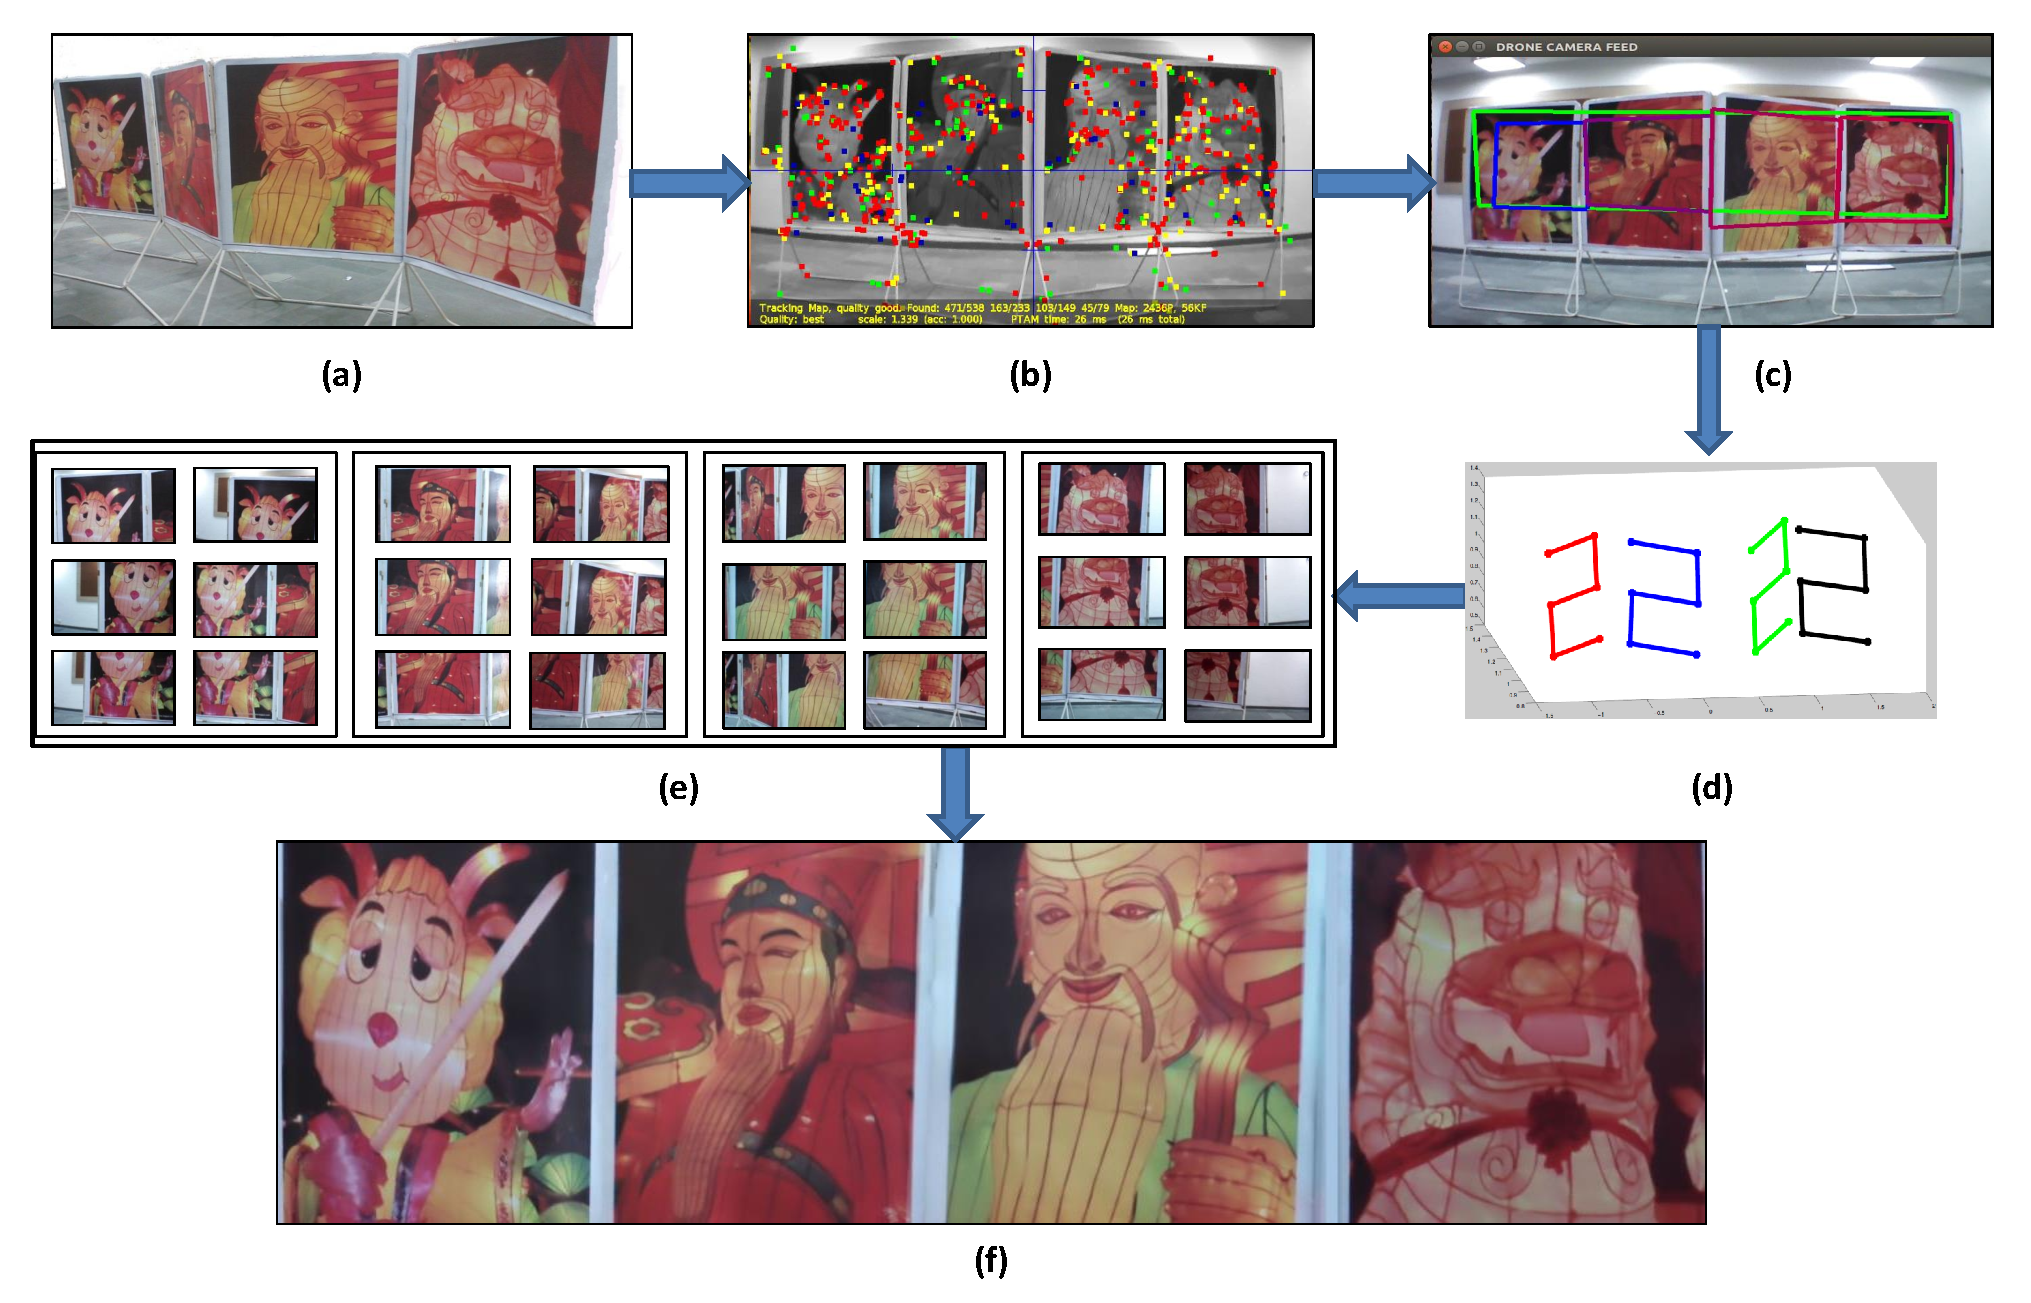
\includegraphics[width=\textwidth]{figures/multiplanar/workflow}
\caption[Overall Workflow]{Overview: (a) Input Scene to be imaged. (b) Feature points in the scene
are found, and their 3D positions are estimated using scale aware PTAM \cite{engel}. (c) Multiple bounded planar
regions are estimated using our algorithm. (d) For each bounded planar region, 3D camera positions
are calculated and overall path planning is done. (e) Videos are captured at
each target position. From each captured video, the appropriate frame is
found. (f) Individual mosaics are joined to get final output.}
\label{fig:workflow}
\end{figure}
\subsection{3D map}
We have used PTAM based method \cite{engel} to localize the quadcopter as well
as to create a 3D map of the surrounding environment (See Figure \ref{fig:ptam_output}).
In PTAM, initially, the prior pose is estimated using motion model. Then, the
map points are projected into the image using prior pose estimate. Next, the camera
pose is updated using some of the feature matches in the image. The final pose
estimate is computed from all the matches found.
 
The initial map built from stereo initialization algorithm has an arbitrary
scale. Hence, there is a requirement of scaling the  map to metric units. This
is done by assuming that the camera is translated 10 cm between the stereo pair. This
assumption may not be true in the case of an inexpensive quadcopter due to its jerky
motions. Hence, proper scale estimation is necessary.

\textbf{Scale Estimation}
A quadcopter measures a distance traveled during translation using PTAM as well
as available metric sensors (ultrasound altimeter) at regular intervals. We get
a pair of samples $\mathbf{x}_i, \mathbf{y}_i \in {\Re}^d$ where $\mathbf{x}_i$ is
scaled translation calculated from the PTAM system and $\mathbf{y}_i$ is the
distance measured by the metric sensor at each interval. These pair of samples are related
according to $\mathbf{x}_i \approx \lambda \mathbf{y}_i$. The scale $\lambda$ is
estimated by minimizing the negative log-likelihood\cite{engel}.  

We could get the correct pose by  scaling  PTAM estimated pose. However, we
cannot rely only on PTAM for pose estimation as visual feedback may lag due to
problems in wi-fi connectivity. Hence, there is a requirement of  alternative
mechanism as a fallback to PTAM. Engel et al. \cite{engel} have used Extended
Kalman Filter to fuse the odometry observation model with the visual observation
model for state prediction, i.e., estimating the pose (x,y,z and roll-pitch-yaw) of 
the quadcopter at any given instant.

\textbf{State Prediction and Observation:} The state space consists of a total
of ten state variables. 
\begin{ceqn}
\begin{align}
	\mathbf{x}_t &\coloneqq {(x_t, y_t, z_t, \dot{x_t}, \dot{y_t},
	\dot{z_t}, {\Phi}_t, {\Theta}_t, {\Psi}_t, \dot{{\Psi}_t} )}^T  \in
	{\mathbb{R}}^{10},
\end{align}
\end{ceqn}
where $(x_t, y_t, z_t)$ represents the position of the quadcopter in
metric units and $(\dot{x_t}, \dot{y_t}, \dot{z_t})$, the velocity in m/s, both
in world coordinates. The state also contains three angles (in degrees), i.e.,
the roll ${\Phi}_t$, pitch ${\Theta}_t$, and yaw ${\Psi}_t$, of the drone. 
An observation function $h(x_t)$ for each sensor as well as respective observation vector $z_t$
composed from the sensor readings is defined for each observation model.

\textbf{Odometry observation model:} A quadcopter measures its horizontal speed
(i.e., along x and y direction) in its local coordinate system which is
transformed into the global coordinate system to get $\dot{x_t}$ and
$\dot{y_t}$. The roll and pitch angles are directly taken from the
accelerometers' observations. Height measurements ($\hat{h_t}$) and yaw measurements
($\hat{{\Psi}_t}$) are differentiated and treated as observations of respective
velocities. The resulting observation function $h_I(\mathbf{x}_t)$ and
measurement vector $\mathbf{z}_{I,t}$ is given by,
\begin{ceqn}

\begin{align}
	h_I(\mathbf{x}_t) &\coloneqq  
	\begin{pmatrix} 
		\dot{x_t}\cos{{\Psi}_t} - \dot{y_t}\sin{{\Psi}_t} \\
		\dot{x_t}\sin{{\Psi}_t} + \dot{y_t}\cos{{\Psi}_t} \\
		\dot{z_t} \\
		{\Phi}_t \\
		{\Theta}_t \\
		\dot{{\Phi}_t}   	
	\end{pmatrix}
	\\
	\mathbf{z}_{I,t} &\coloneqq (\hat{v}_{x,t}, \hat{v}_{y,t}, (\hat{h}_t -
	\hat{h}_{t-1}), \hat{{\Phi}_t}, \hat{{\Theta}_t}, (\hat{{\Psi}_t} - \hat{{\Psi}}_{t-1}  ) )^T
\end{align}
\end{ceqn}
\textbf{Visual Observation Model:} The pose estimate is scaled by the
current estimate for the scaling factor ${\lambda}^{*}$ when PTAM tracks a
video frame successfully. This pose estimate is transformed from the coordinate
system of the front camera to the coordinate system of the quadcopter. Direct
observation of the quadcopter’s pose is given by,
\begin{ceqn}

\begin{align}
	  h_P(\mathbf{x}_t) &\coloneqq  {(x_t, y_t, z_t, {\Phi}_t, {\Theta}_t,
	  {\Psi}_t)}^T \\
	  \mathbf{z}_{I,t} &\coloneqq
	  f(\mathbf{E}_{\mathit{DC}}\mathbf{E}_{\mathit{C},t} )
\end{align}
\end{ceqn}

where $\mathbf{E}_{\mathit{C},t} \in SE(3)$ is the estimated camera pose (scaled
with $\lambda$ ), $\mathbf{E}_{\mathit{DC}} \in SE(3)$ the constant
transformation from the camera to the quadcopter coordinate system, and $f :
SE(3) \rightarrow \mathbb{R}^6$ the transformation from an element of $SE(3)$ to
our roll-pitch-yaw representation.

\textbf{Prediction Model:} The Extended Kalman filter is used to fuse all state
variables from both observation models. (Please see \cite{engel} for the
details). Finally, the prediction model describes how state vector $\mathbf{x}_t$
evolves from one timestep to next. The quadcopter’s horizontal acceleration $\ddot{x}, \ddot{y}$ is
approximated based on its current state $\mathbf{x}_t$.
The quadcopter's vertical acceleration   $\ddot{z}$, yaw-rotational 
acceleration $\ddot{{\Psi}_t}$ and roll and pitch rotational speeds,
$\dot{{\Psi}_t}, \dot{{\Theta}_t}$ are estimated based on the state
$\mathbf{x}_t$ and  active control command $\mathbf{u}_t$. Finally, using quadcopter's 
estimated pose information, we update the 3D map of the environment.

\noindent\textbf{Scale Accuracy:} 
Though \cite{engel}  gives a 3D map of the environment, the scale accuracy is
not ensured. It leads to inaccurate 3D coordinates of feature points. However, we
require accurate 3D coordinates of the region to be imaged for successful path
planning and its execution. To ensure accurate scale, we moved the quadcopter autonomously in
the vertical direction (up and down) by fixed distance. The reason behind moving in
the vertical direction is that the sonar gives us very accurate height information 
which is used to remove scale ambiguity.

We have conducted a small experiment to demonstrate the efficacy of our method to
achieve high scale accuracy. First, we initialized PTAM after
taking off the quadcopter, moved the quadcopter to location (0, 0, 1), i.e., 1
meter above the ground, and finally landed it at the same location. Ideally,
take-off location and land location should be same. However, due to errors in
PTAM initialization as well as noise in IMU measurements, the distance between
two locations will be non-zero. We use this distance as a measure of error. We
also tried to imbalance the quadcopter, while it is at location (0, 0, 1),
before landing to check its ability to come back to the original position.

Later, we repeated the experiment with one change, instead of using only PTAM
initialization, we have autonomously moved the quadcopter up and down by fixed
distance (1 meter) after PTAM initialization. Our summarized observations
after ten runs in both cases are listed in the Table~\ref{tab:ptamInit}.
\begin{table}
\centering
\newcolumntype{C}{ >{\centering\arraybackslash} m{2cm} }
\newcolumntype{D}{ >{\arraybackslash} m{5cm} }
\begin{tabular}{|D|C|C|C|C|}
\hline
\centering Case & Avg. Scale Accuracy & Avg. Scale (in m) & Number of Iterations &
Mean Error $\pm$ std. (in cm)\\
\hline
Only PTAM initialization & 0.524 & 1.2 & NA & 82.6 $\pm$ 10.73 \\
\hline
PTAM initialization with accuracy check & 1.0 & 2.33 & 3--4 & 13.2 $\pm3.6$\\
\hline       
\end{tabular}
\caption[Effect of ensuring scale accuracy on pose estimation]{Effect of
ensuring scale accuracy on the pose estimation of a quadcopter.
The first row shows that with only PTAM initialization, we do not get an accurate pose.
When we use our method to ensure high scale accuracy, we are much better in
pose estimation. The scene used for this testing was 2.3 meters away from the
quadcopter. As the estimated scale (2.33m) with our method is very close to the
actual distance of the scene from the quadcopter, the generated 3D map is also
very accurate.}
\label{tab:ptamInit}
\end{table}
Table~\ref{tab:ptamInit} clearly indicates that the pose estimate with only PTAM
initialization is far off (around 85cm) from the actual position\footnote{We also
noted that sometimes quadcopter was not able to come anywhere near to (0, 0, 1)
if we imbalance quadcopter purposefully after PTAM initialization.}.
However, when we ensure high scale accuracy, the estimated pose is within 15cm
of the actual location. The estimated scale is also very close to the actual distance of
the plane if we use our method for ensuring scale accuracy.

\begin{figure}[t!]
\centering
\includegraphics[width=\linewidth]{images/3D_2D}
\caption[Creation of 3D map]{Mapping of 3D locations to 2D image pixel locations
of feature points using PTAM. Left: Camera view showing 2D locations of detected feature points.
Color coding indicates the coarseness level of detected features. Right: Mapview
showing 3D locations of detected feature points.}
\label{fig:ptam_output}
\end{figure}

\subsection{Human Interaction}
Next step after we get a 3D map of the environment is getting the desired area for
imaging from the user. The user may be interested in a particular part of
the scene spread over multiple planes. Hence, we have to identify the user's
area of interest on the multiplanar surface. We first fly the quadcopter at a
sufficiently far distance from the surface. The distance should be such that the user can see the whole
scene. The user marks the area of interest with the provided user interface.\\
\begin{figure}[t!]
\centering
\includegraphics[width=0.31\linewidth]{images/UI_input}
\includegraphics[width=0.31\linewidth]{images/UI_points_marked}
\includegraphics[width=0.31\linewidth]{images/UI_convexHull}
\caption[Our user interface]{Left: The user is shown a live video stream as seen
from a quadcopter camera. Middle: The user may click points to denote the area of interest. We 
find out the nearest 3D point and show its projection (encircled blue pixels) on
the image plane. Right: Once user finishes with clicking points, we find out its convex
hull and show it in green convex polygon.}
\label{fig:ui}
\end{figure}
\textbf{User interface} Users are shown the live video stream as seen through
the quadcopter (Figure \ref{fig:ui}(Left)). Now, users can click points to
mark their area of interest on the 2D screen. At the backend, we determine the
nearest 3D point corresponding to the location clicked by the user and then show
its projection on the image plane. (Figure \ref{fig:ui}(Middle)). Once they
finish marking the points, they can see the convex hull of the
clicked points to check whether the area to be covered is indeed the area of
interest (Figure \ref{fig:ui}(Right)). The user can optionally add or delete points
or even completely remove all clicked points using the interface and select the
new ones.

\subsection{Multiplanar Regions Detection}
We have to detect multiple planes present in the user's region of
interest. There are many algorithms such as Sequential RANSAC\cite{Kanazawa},
multiRANSAC\cite{zuliani} , J-linkage\cite{jlinkage}, T-linkage\cite{tlinkage}
etc. to detect multiple models from the data. We have chosen a real-time
implementation of J-linkage \cite{realtimejlinkage}.\\
\textbf{J-linkage:} Sequential RANSAC and multiRANSAC algorithms require
the number of planes as an input parameter. However, as the number of planes
change according to the input scene, we cannot use these algorithms. J-linkage and T-linkage
doesn't require the number of planes as an input parameter. 
%Though T-Linkage is more robust to noise in the input points, it is an order of
%magnitude slower than J-linkage. 
Our application requires real-time detection of the number of planes before proceeding for 
actual capture. This makes J-linkage more suitable than T-linkage.

However, J-linkage doesn't give the extent of the plane, i.e., the bounded
region. It tries to fit all points to the planes. Figure \ref{fig:multiplane}
depicts the relevant scenario. As we can see, there are some points which may
be the result of an inaccurate 3D map generated by PTAM (indicated by the black oval).
As these points have ``geometric'' affinity towards the plane A, J-linkage puts
these points in the plane A\textquotesingle s cluster. However, in the real world they
are part of the plane B. Hence, we have to disambiguate such points for
the correct calculation of bounded multiplanar regions. We have developed an
algorithm to modify the output of J-linkage to give correct bounded multiplanar regions.\\
\textbf{Improvement over J-linkage:} J-linkage algorithm outputs label
for each data point denoting to which plane that data point belongs. Our
algorithm does the following to find continuous bounded multiplanar regions
from J-linkage output:
\begin{itemize}
  \item Run clustering algorithm, e.g., k-means using the output of J-linkage
  as initial labels.
  \item Find out the distance of all points inside each cluster from the cluster
  centroid along the normal of the given plane.
  \item Remove the points from the cluster which are more than 95 percentile
  farther from the cluster centroid along the plane normal.
  \item Find out the bounding rectangle of each cluster.
  \item Extend the rectangle till the intersection with the successive plane.
\end{itemize}

This process is illustrated in Figure \ref{fig:multiplane}. J-linkage
gives us the labeling according to each point's vicinity to the detected
planes. However, the 3D points estimated by PTAM may be erroneous due to noise,
marked by circles in Figure \ref{fig:multiplane}(Top). J-linkage gives us wrong bounded
regions as these points do not belong to the planes labeled by it . Hence, we
run the k-means algorithm using the initial labels given by JLinkage. Now, points  
belong to the correct cluster as shown in Figure \ref{fig:multiplane}(Middle). 
However, we don't want points which are far away from the plane in the normal direction.
Hence, we remove those points which are more than 95 percentile farther from the cluster 
centroid along the plane normal. We also trim the boundaries of the plane by
the bounding box of the enclosed points. The final output is shown in the
Figure \ref{fig:multiplane}(Bottom).

\begin{figure}[h!]
\centering
\includegraphics[width=\linewidth]{figures/multiplanar/multiplaneDetection}
\caption[Process of finding bounded multiplanar regions from J-linkage
output.]{Process of finding bounded multiplanar regions from J-linkage output.
The top image shows us the initial labeling given by J-linkage. Later, we run
the k-means algorithm using the initial labeling given by J-linkage. The output
is shown in the middle figure. Finally, we remove outliers which are farther
from the plane along normal direction and trim boundaries of the plane as shown
in the bottom figure.}
\label{fig:multiplane}
\end{figure}

Each bounded planar region is used to determine the path along which
the quadcopter is navigated to image that region.

\subsection{Path Planning}
The bounded region is divided into a grid of overlapping cells as shown in
Figure \ref{fig:grid}. We intend to cover each cell in a single image and then
use images from all cells to create a mosaic of a given bounded planar
region. The cell area (width, height) is decided on the basis of the amount of
details required of the scene. For example, if we have to probe our scene with
minute details, we have to go nearer to the plane. Hence, in that case, the
cell area is smaller. We require an overlap between neighboring images for
successful mosaicing. The amount of overlap between two cells is a function of
the required overlap in the feature space required for stitching. Currently,
the overlap is set at thirty percent of the cell area to deal even with sparser
(containing very fewer feature points) images.

\begin{figure}[h!]
\centering
\includegraphics[width=\linewidth]{figures/multiplanar/PathPlanningGrid}
\caption[Creation of Grid for Path planning]{Grid of overlapping cells designed
for path planning. We create a grid for each bounded planar region. The cell width and the cell height is
decided based on the area we would like to capture in one frame. Overlap parameter is
a function of overlap required in feature space for successful stitching.
We find the camera position for each cell in the grid which in turn
gives us the path for a quadcopter to image the given bounded planar region.}
\label{fig:grid}
\end{figure}

Once we calculate coordinates of cell corners, we determine the desired position of
a camera from where the whole cell area is covered in a single image. It is
illustrated in the Figure~\ref{fig:solvepnp}. The coordinates of corner points
are decided on the basis of cell width, cell height and the top-left corner of
the cell. The image coordinates (in pixels) depends on the size of the image. We
pose this problem as a point correspondence problem to estimate the position
of the camera. We repeat this process for each cell to find out the waypoints of
the path of a quadcopter to cover the region in optimal (in a number of positions)
manner, so that the whole region is captured.

\begin{figure}[h!]
\centering
\includegraphics[width=\linewidth]{figures/multiplanar/SolvePnP}
\caption[Estimating camera position to capture the cell area in one
image]{Finding the camera position for capturing the desired cell area in a single image. Note that, imaging area coordinates are in metric units, while image
coordinates are in pixels. We use point correspondence problem to estimate the
camera position.}
\label{fig:solvepnp}
\end{figure}

\subsection{Navigation of a quadcopter}
 We use the pose estimate provided by PTAM  based method \cite{engel}to track
 the quadcopter during navigation along the planned path.\\
\textbf{Covering a bounded single planar region}:
We navigate the quadcopter smoothly in a ``snake scan'' manner along the target points estimated in path
planning step to cover each bounded planar region.\\
\textbf{Transition from one plane to another plane}: We make sure the
transition in terms of yaw as well as horizontal movement is smooth. To achieve this,
we divide the horizontal distance into three parts and  move along x-axis and y-axis
alternatively. During each step, we change the yaw in equal proportion so that
the quadcopter’s view is not changed drastically, which is very important for
tracking using PTAM \cite{engel}.

\subsection{Recording video and ROS streams}
%AR Drone doesn't have the capability of taking still photographs. 
 We are not sure about the exact position of a quadcopter while capturing
 images due to the error in PTAM as well as the jerky motion of a quadcopter. 
 Hence, instead, we record a video on the USB device onboard a quadcopter for a
 small amount of time (3 seconds) when we are in proximity of each point in the calculated path. We
also record ROS streams (image as well as positional data) captured over Wi-Fi.

\noindent\textbf{Finding the sharp and exact image from video:} We have to find
the sharp image, i.e., an image with the minimum blur which is closest to the
target point from 3 seconds HD video (approximately 90 images) to create a
mosaic. However, there is no positional data available on USB device. Positional
data stream and image stream captured over Wi-Fi help us in this process. First, we synchronize these
two streams captured over Wi-Fi using timestamp information. It gives us an
approximate position of each image from the image stream captured over Wi-Fi.
Now, we select the sharpest image among the images captured over Wi-Fi which
are taken from the positions in a proximity of the specified point. Later,
we match each image from the HD video (recorded on USB device) with the
selected image (selected from the Wi-Fi image stream) using SURF features. It
gives us a subset of HD images which are within a threshold in SURF\cite{Bay} feature
space from the selected image. Finally, we select the sharpest image from that subset of HD images.

\subsection{Creating mosaic of the bounded multiplanar region}
Once images for each bounded planar region are extracted from captured
videos, mosaic for each planar region is created using the method of creation of
a mini-panorama presented in \cite{Prasad16}. In \cite{Prasad16}, first images
are arranged in a rectangular grid according to their positions. Here, as we
already have grid information (created in path planning step), our first step
is done. Later, we do feature matching among the neighborhood images and create
the maximum spanning tree using the homography inliers as weight.  Finally,
mosaic, i.e., mini-panorama is created by warping images according to the
respective homography matrix (w.r.t. the  reference image).

\begin{figure}[ht!]
\centering
\includegraphics[width=\linewidth]{figures/multiplanar/SinglePlaneMosaic}
\caption{Super panorama creation by finding the disparity between reference
images of mosaics imaged on a single plane~\cite{Prasad16}.}
\label{fig:singlePlaneMosaic}
\end{figure}

After the creation of mini-panorama for each planar region, we join all
mini-panoramas using a method similar to the creation of super panorama used
in~\cite{Prasad16}. Super panorama is created by forming a simplistic stereo
pair between two images captured from the same depth, as shown in
Figure~\ref{fig:singlePlaneMosaic}. Using the stereo disparity formula, 
\begin{ceqn}
\begin{align}
\textit{disparity} = \textit{focal
length}\frac{\textit{baseline}}{\textit{depth}},
\label{eq:disparityOrig}
\end{align}
\end{ceqn}
we can ``place,'' from the first viewpoint, the image captured from the second
viewpoint, thereby creating a super-panorama. In~\cite{Prasad16}, the disparity
between the reference images of each mini-panorama is calculated by using the
distance between the camera and the imaging plane, i.e., the depth, and distance
between camera positions of reference images for each mini-panorama, i.e., the
baseline.

\begin{figure}[ht!]
\centering
\includegraphics[width=\linewidth]{figures/multiplanar/MultiplanarMosaic}
\caption{Process of finding the disparity between reference images of mosaics
imaged on two different planes.}
\label{fig:multiplanarMosaic}
\end{figure}

In~\cite{Prasad16}, as all mini-panoramas were in the same plane, simple stereo
formulation (without rectification) was enough. In our case, as mini-panoramas belong to
multiple planes, we have to project mini-panoramas on any one plane to find the
disparity between reference images of all mini-panoramas. It requires image
rectification. However, as we keep the quadcopter's camera normal to the plane
while capturing images from each planar region, we don't have to do full
rectification. We just have to calculate the distance between the center of
projections, projected on the imaging plane, along the planes as shown in
Figure \ref{fig:multiplanarMosaic}.

Let us assume that the depth of the camera from both the imaging planes is same
(say $Z$). Now, the disparity of the image on the second plane with respect to
the image on the first plane is given as follows:
\begin{ceqn}
\begin{align}
\textit{disparity} = \textit{focal length}\frac{(d_1+d_2)}{Z},
\label{eq:disparity}
\end{align}
\end{ceqn}
where $d_1$ and $d_2$ are distances of projections of camera positions on the
first and second plane respectively, from the line of intersection of two
planes, and $Z$ is the depth of the camera from the plane.
If we compare Eq.~\ref{eq:disparityOrig} and Eq.~\ref{eq:disparity}, we can 
easily see that, now our baseline is $(d_1 + d_2)$, i.e., distance between
camera positions calculated along the plane, instead of calculating the direct 
distance between camera positions. The reason behind this difference is, imaging
areas are on two different planes instead of one.

If the center of projections are at different depths (e.g., say $Z_1$ and
$Z_2$), first we bring the image captured from lesser depth (say $Z_1$) to the
same depth of another image (which is captured from larger depth, say $Z_2$) by
zooming out by the fraction $\frac{Z_1}{Z_2}$. Later, we use Eq.
\ref{eq:disparity} to calculate the disparity by setting $Z=Z_2$.

To summarize, our method first creates an accurate 3D map of the input scene
spread over multiple planes using extended PTAM initialization. Next, we determine the
boundaries of each planar region using the improvised J-linkage algorithm.
Further, we estimate the optimal number of positions along which we will navigate the
quadcopter to capture videos which encompass the complete scene. Later, we
create the individual mosaics for each plane with the images extracted from
videos. Finally, the individual mosaics are joined using super-panorama
formulation to get an unrolled view of the input scene.

\section{Experiments and Results}
All our experiments have been completed with the inexpensive consumer
quadcopter called  Parrot’s AR Drone 2.0. The camera resolution of AR Drone 2.0
is 1280 $\times$ 720\footnote{But when we stream the image over Wi-Fi the resolution
of an image is 640 $\times$ 360.}. We have used ROS based ARDrone Autonomy
Driver~\cite{ardroneDriver} to communicate with the drone. We have also used
tum\_ardrone package~\cite{tumardrone} for ROS to do PTAM based state
estimation. We have developed an ROS node for autonomous navigation of
quadcopter. The code is developed in C++ and will be made available at
after acceptance of the paper. Mosaicing algorithm is also
developed in C++ using the OpenCV library (OpenCV 2.4.9). Experiments were
performed on a laptop with Intel Core i5 processor(@2.4GHz) and 8GB RAM.

We also took a picture of the scene, from a distance with a five mega-pixel
camera to better understand the scene as well as to show the efficacy of
our method.

\subsection{Single Plane with Multiple Visits}
We have first used our algorithm to image a single planar wall shown in
Figure \ref{fig:resultLady}(Left). As the wall was too tall and it was not
possible to view the full wall in one flash due to a shortage of space, we
selected the desired area in two steps as shown in Figure  \ref{fig:resultLady}(Middle). In path planning 37 (12
for the top part and 25 for the bottom part) positions were estimated to
encompass the user-selected area. Images captured from those positions are
mosaiced using our algorithm to get the final mosaicing output as shown in Figure \ref{fig:resultLady}(Right).
\begin{figure}
\centering
\includegraphics[width=0.9\textwidth]{figures/multiplanar/ladyResult.pdf}
\caption[Result: Single Plane]{There is a 15 feet tall wall as shown in the
long-range photograph (left) which we would like to image orthographically with details. We cannot
select the whole area in a single instance as we cannot go back to see the whole
wall. Hence, we selected the desired area in two steps as shown in GUI for area
selection (middle-top and middle-bottom). Green quadrilateral shows user selected area
while blue quadrilateral shows the bounded planar region estimated by our
algorithm. In path planning 37 (12 for the top part and 25 for the bottom part) positions were
estimated to encompass the user-selected area. Images captured from those
positions are mosaiced using our algorithm to get the final mosaicing output as shown in the
right image.}
\label{fig:resultLady}
\end{figure}

\subsection{Multiple Planes}
Our further experiments are done on various setups covering multiple planes.\\

\textbf{Concave:} In this experiment, the exhibits were arranged in the concave
fashion as shown in Figure \ref{fig:resultConcave}(Top-Left). We have selected
the area to be imaged as shown in Figure \ref{fig:resultConcave}(Top-Right). In
the path planning stage, overall 27 (9 from the left plane, 12 from the middle
plane, and 6 from the right plane) positions were estimated to encompass
user-selected area. Images captured from those positions are mosaiced using our
algorithm to get the final mosaicing output as shown in the Figure \ref{fig:resultConcave}(Bottom).

\begin{figure}
\centering
\includegraphics[width=\linewidth]{figures/multiplanar/ConcaveResult.pdf}
\caption[Result: Concave arrangement]{There is an art exhibition containing
multiple posters arranged in concave fashion as shown in the long range photograph (top-left). We have
selected the area to be imaged as shown in GUI for area selection(top-right).
Green quadrilateral shows user selected area while blue, violet and magenta
colored quadrilaterals represent the multiple bounded planar regions
estimated by our algorithm. In the path planning stage, overall 27 (9 from the left
plane, 12 from the middle plane, and 6 from the right plane) positions were
estimated to encompass the user-selected area. Images captured from those
positions are mosaiced using our algorithm to get the final mosaicing output as shown in the bottom image.}
\label{fig:resultConcave}.
\end{figure}

\textbf{Convex:} In this experiment, paintings were arranged in the convex
fashion as shown in Figure \ref{fig:resultConvex}(Top-Left). We have selected
the area to be imaged as shown in Figure \ref{fig:resultConvex}(Top-Right). In
the path planning stage, overall 30 (9 from the left plane, 12 from the middle
plane, and 9 from the right plane) positions to encompass user-selected area are
estimated. Images captured from those positions are mosaiced using our algorithm to get the final
mosaicing output as shown in the Figure \ref{fig:resultConvex}(Bottom).

\begin{figure}[t!]
\centering
\includegraphics[width=\linewidth]{figures/multiplanar/convexResult.pdf}
\caption[Result: Convex arrangement]{There is an exhibition of Indian temple
paintings arranged in convex fashion as shown in the long range photograph (top-left). Note that we
cannot cover all paintings with enough details simultaneously. We have selected
the area to be imaged as shown in GUI for area selection (top-right).
Green quadrilateral shows user selected area while blue, violet and magenta
colored quadrilaterals represent the multiple bounded planar regions
estimated by our algorithm. In the path planning stage, overall 30 (9 from
the left plane, 12 from the middle plane, and 9 from the right plane) positions were
estimated to encompass the user-selected area. Images captured from estimated
positions are mosaiced using our algorithm to get the final mosaicing output as shown in
the bottom image.}
\label{fig:resultConvex}
\end{figure}

\textbf{Mixed:} We have performed a couple of experiments where the posters were
arranged in mixed fashion. The first arrangement looked like Figure
\ref{fig:resultMixed1}(Top-Left) where the middle posters form the convex region
while the side posters form the concave region. The selected area for imaging is
shown in Figure \ref{fig:resultMixed1}(Top-Right). In path planning overall 24 (6 from each
plane) positions are estimated to encompass the user-selected area. Images
captured from those positions are mosaiced using our algorithm to get the final mosaicing
output as shown in the \ref{fig:resultMixed1}(Bottom).

\begin{figure}[t!]
\centering
\includegraphics[width=\linewidth]{figures/multiplanar/mixed1Result.pdf}
\caption[Result: Mixed arrangement]{There is an exhibition of Chinese lanterns'
posters arranged in mixed (concave and convex) fashion as shown in the long range photograph
(top-left). Note that we cannot cover all paintings with enough details
simultaneously. We have selected the area to be imaged as shown in GUI for
area selection (top-right). Green quadrilateral shows user selected area while
blue, violet and magenta colored quadrilaterals represent the multiple
bounded planar regions estimated by our algorithm. In the path planning overall
24 (6 from each plane) positions were estimated to encompass the user-selected
area. Images captured from estimated positions are mosaiced using our algorithm to get the
final mosaicing output as shown in the bottom image.}
\label{fig:resultMixed1}
\end{figure}

In the second mixed arrangement, middle posters form the concave region while
 side posters form the convex region as shown in Figure
\ref{fig:resultMixed2}(Top-Left). The selected area for imaging is shown in
Figure \ref{fig:resultMixed2}(Top-Right).  In path planning overall 24 (6 from
each plane) positions were estimated to encompass the user-selected area.
Images captured from estimated positions are mosaiced using our algorithm to get the final mosaicing
output as shown in the Figure \ref{fig:resultMixed2}(Bottom).

\begin{figure}
\centering
\includegraphics[width=\linewidth]{figures/multiplanar/mixed2Result.pdf}
\caption[Result: Mixed arrangement]{There is an exhibition of Chinese lanterns'
posters arranged in mixed (concave and convex) fashion as shown in the long range photograph
(top-left). Note that we cannot cover all paintings with enough details
simultaneously. We have selected the area to be imaged as shown in GUI for
area selection (top-right). Green quadrilateral shows user selected area while
blue, violet and magenta colored quadrilaterals represent the multiple
bounded planar regions estimated by our algorithm. In the path planning
stage, overall 24 (6 from each plane) positions were estimated to encompass the
user-selected area. Images captured from estimated positions are mosaiced using
our algorithm to get the final mosaicing output as shown in the bottom image.}
\label{fig:resultMixed2}
\end{figure}

\textbf{Planes at different depth:} In this experiment we have arranged posters
parallel to each other, but at different depths, as shown in Figure
\ref{fig:resultFrontBack}(Top-Left). It is not possible to mosaic them together
due to change in planes. However, we have imaged each exhibit independently
using quadcopter and brought the mosaic of the exhibit at a larger depth to the same depth
of lesser depth exhibit mosaic using the estimated plane equations' information.
The final result is shown in the Figure \ref{fig:resultFrontBack}(Bottom).
\begin{figure}
\centering
\includegraphics[width=0.9\textwidth]{figures/multiplanar/frontback.pdf}
\caption[Result: Imaging at different depths]{There are two Chinese lanterns'
exhibits, arranged parallel to each other but having different depths as shown in the long-range
photograph(top-left). It is not possible to mosaic both of them in a single
panorama due to the difference in depths. We imaged those exhibits
independently through a quadcopter and brought the mosaic of the exhibit at larger
depth to the same depth of lesser depth exhibit mosaic. The final result is
shown in the bottom image.}
\label{fig:resultFrontBack}
\end{figure}

\section{Concluding remarks}
We have developed an end-to-end application for autonomously imaging multiplanar
regions using quadcopter. We have also developed an algorithm for `unrolling'
the multiplanar scene using the fusion of IMU data and video captured from
a quadcopter. Homography-based stitching cannot be used to create the mosaic of
scene spread over multiple planes. Also, using the handheld camera is cumbersome
to cover large multiplanar surfaces. Even with the UAVs manual control is very difficult.

In our solution, we autonomously maneuver a quadcopter along the planned path to
capture each plane in the multiplanar surface. The path planning for each plane
is done to estimate optimal locations such that images from the estimated
locations will cover the whole plane. Later, we stitch images for each plane to create a mini-panorama.
Finally, mini-panoramas are merged using positional information to form a full panorama.
Our method works in various setups like convex, concave as well as mixed.

%In the future, our method may be extended to cover any parametric surface in
%general.
It is practically impossible to image very large multiplanar surface using
just single quadcopter due to battery constraint. We can use multiple
quadcopters in collaboration to overcome this limitation. However, we need to
identify each quadcopter accurately to send proper commands. Identification of
a moving object in the unknown environment is a challenging task. Generally, 
fiducial markers are placed on an object for tracking. Motion blur introduced
due to swift movements of quadcopter causes problem in detection of current
fiducials. We discuss the design of motion blur resilient fiducials as well as
the detection of the same in next chapter.

\chapter[Blur Resilient Fiducials]{A Motion Blur Resilient Fiducial For
Quadcopter Imaging}
\label{ch:fiducial}

The recent availability of low-cost quadcopters such as ARDrone 2.0 has helped 
fuel significant efforts in research focused on unmanned aerial
vehicles. Navigation and planning
of these vehicles is typically~\cite{Davison:2007,Engel12,Engel13}
performed using onboard inertial sensors and/or vision based modules
that uses visual cues in the real world. However, to evaluate the
effectiveness of navigation methods, one or more fiducials are commonly
placed~\cite{Bosnak:2012,Lim09,Klopschitz:2007}
 in the environment to provide additional information that
serves for ground-truth positional measurements.
In order to be effective, fiducial markers (or simply, fiducials) need
to be easily recognized in the scene. A variety of fiducials have
been proposed~\cite{NaimarkF02,ARToolkit02,Fiala05,Pitag13,runetag11}
in the literature.  These take the form of binary codes arranged into
rectangular grids~\cite{ARToolkit02,Fiala05} or other geometric
primitives arranged in predefined spatial
patterns~\cite{NaimarkF02,Pitag13,runetag11}.  Figure \ref{fig:fiducial_teaser}
shows the popular ARTag \cite{Fiala05} fiducial as possibly seen from
a quadcopter.

\section{Introduction}
\label{sec:intro}
 A problem for existing fiducials is that low-cost
quadcopters often exhibit very quick and erratic physical movements
that result in motion blur evidenced in the images captured from the quadcopter's onboard
camera. This motion blur has an adverse effect on the recognition of fiducial
markers. This can be seen in Figure \ref{fig:fiducial_teaser}--(b) where the
ARTag fiducial cannot be recognized due to motion blur. This is not
too surprising as most existing fiducials are not designed to handle
motion blur.

Compounding this problem is the additional issue of dropped video
frames from the quadcopter's wireless communication module. This means
that not only is blur a problem, but there may be large
discontinuities in the pattern's position due to missing video
frames. This problem makes it challenging to apply tracking algorithms that can
exploit temporal coherence for determining the fiducial's position.

\noindent\textbf{Contributions:}~~To address these problems, we propose a
fiducial that is designed to be resistant to motion blur. Our design
is based on circles as shown in Figure~\ref{fig:fiducial_teaser}--(c,d). The
design is based on the observation that motion blur from a quadcopter
tends to be linear in nature. As such, when our fiducial is blurred,
there is no blur in the direction perpendicular to the direction of
motion.  This allows the signature of the fiducial to remain intact in
any direction.

When multiple fiducials are present, using concentric rings, we can
treat the presence or absence of a ring as a bit, allowing us to
assign a code to the marker. Our experiments show that these designs can
significantly outperform existing codes in the presence of motion
blur. As far as we are aware, this is the first work to propose a blur
resistant marker, especially in quadcopter settings.

%The remainder of this chapter is organized as follows.  Section~2 gives
%an overview of related work in fiducials, as well as the related
%problem of tracking. Section~2 motivates our fiducial design by
%analyzing the performance of existing codes under motion blur, and
%describes our detection algorithm. Section~3 shows several
%experiments using quadcopter imagery. This is followed by a discussion
%and a summary in Section~4 and Section~5 respectively.

\begin{figure}[t!]
  \includegraphics[width=\linewidth]{figures/fiducial/teaser}
  \caption[Overview]{Experimental setup and comparison of fiducial-based
    algorithms. A green border signifies success. 
    \textbf{(Left)} A drone encounters three different fiducials. 
    \textbf{(Right, Top)} Output of ALVAR~\cite{alvar} under favorable and blurred
    circumstances. No green border is seen in (b) signifying failure.
    \textbf{(Right, Bottom)} Output of the proposed fiducial. Green
    border is seen in both (c) and (d).
    \label{fig:fiducial_teaser}}
  \end{figure}

\section{Design of Blur Resistant Fiducial}

We begin by first motivating the need for a new blur resistant
fiducial by examining the performance of prior fiducials under motion
blur.  After this, we detail our design as well as the recognition
algorithm used to find the fiducial in an image, or a video sequence.

\subsection{Prior Fiducials Under Motion Blur}\label{sec:blurtest}

Here we examine the performance of two popular fiducials under
motion blur.  Specifically, we examine ARTags ~\cite{Fiala05} and
PiTags~\cite{Pitag13} given their differences in geometric design and
the availability of an API to develop applications to recognize the tags.
\footnote{RUNE-tag~\cite{runetag11} currently does not
provide access to an implementation to generate or recognize its tags. 
The circular data matrix~\cite{NaimarkF02} is available as a
commercial product, however it requires proprietary hardware.}

%To evaluate the ARTag and PiTag under blur, 
For controlled study, we simulate the appearance of the ARTag and PiTag
markers by scaling the tags to 150$\times$150 pixels.
Both fiducials are then blurred using linear motion blur at various
orientations with different  blur scales. The blur motion ranged from 15 to 50
in magnitude (measured in pixels), representing small to significant motion
blur. Figure~\ref{fig:artag_pitag} shows the visual appearance of the blurred
tags. We then try to detect the markers using the ALVAR library~\cite{alvar} and
PiTag library~\cite{ros_pitag}. The table in %the right side of
Figure~\ref{fig:artag_pitag} shows the recognition rate (in
percentage) of the two fiducials at various blur scales over all  orientations.
As we can see, the PiTag performance quickly diminishes under small amounts of
blur, while at 35 units, the ARTag's recognition rate drops to less than
20\%.

\begin{figure}[t!]
\includegraphics[width=\linewidth]{figures/fiducial/artag_pitag.pdf}
%\captionof{figure}{Blurred ARTag and Pi--tag with various blur scales}
%\captionof{table}{Recognition rate of ARTag and Pi-tag fiducial at various blur scales}

\begin{tabularx}{\linewidth}{|Y|Y|Y|}
\cline{1-3}
\small{Blur} & \multicolumn{2}{c|}{ \small{Recognition Rate}}
\\\cline{2-3}
\small{Scale}& \small{PiTag} &	\small{ARTag} \\ \cline{1-3}
\small{15} & \small{100} & \small{100} \\ %\cline{1-3}
\small{30} & \small{0} & \small{100} \\  %\cline{1-3}
\small{35} & \small{0} & \small{19} \\ %\cline{1-3}
\small{50} & \small{0} & \small{0} \\ \cline{1-3}
\end{tabularx}
\captionof{figure}[Comparison with PiTag and ARTag]{\textbf{Top:} The PiTag and
ARTag fiducials blurred with various blur scales at different orientations. \textbf{Bottom
    Table:} Recognition rate (in percent). We see that the recognition
  rates for both the tags are significantly reduced. For severe blur,
  recognition fails.}
\label{fig:artag_pitag}
\end{figure}

\subsection{Blur Resistant Fiducial}

We propose a binary coded fiducial that uses concentric white rings of
equal widths on a black background with a blurred
border\footnote{Obviously, this design can be inverted to have a white
  background with black rings.}. The outermost and innermost rings
represent the start and end of the code and are embedded in the
fiducial.  The binary code is represented by the presence (or absence)
of rings between ``marker'' rings.

\begin{figure}
\centering
  \includegraphics[width=.24\linewidth]{figures/fiducial/newconcentric_00.pdf}
  \includegraphics[width=.24\linewidth]{figures/fiducial/newconcentric_01.pdf}
  \includegraphics[width=.24\linewidth]{figures/fiducial/newconcentric_10.pdf}
  \includegraphics[width=.24\linewidth]{figures/fiducial/newconcentric_11.pdf}
  \caption[Two-bit binary  fiducials]{Two bit binary  fiducials representing,
  from left to right 00, 01, 10, and 11.}
  \label{fig:fiducials}
\end{figure}

Depending on which ring is present or absent, the resulting binary
code will change. The number of different patterns depends on the
number of bits in the binary code. For example, if the binary code has
three bits, there will be a maximum of three rings between marker
rings and we end up with eight different patterns.
Figure~\ref{fig:fiducials} shows two-bit binary fiducials.


Our fiducial recognition strategy is different from
\cite{NaimarkF02,Pitag13} and works under significant amounts of blur.
As previously mentioned, our approach works under the observation that
the motion blur for the quadcopter's camera can be well modeled as
linear motion.  This linear motion blur assumption has been shown to
be reasonable in prior works~\cite{Moshe:2003,Moshe:2004}
targeting camera motion blur. Under this assumption, the scene
content perpendicular to the blur direction is unaffected by the blur.
Because of our circular design, the direction perpendicular to the
linear motion will still be recognizable as a linear pattern.
Figure~\ref{fig:blur_direction} shows examples of this using a pattern
under 
various motion directions.

\begin{figure}[h!]
\centering
\includegraphics[width=\linewidth]{figures/fiducial/blur_direction}
\caption{Change in blur direction changes the location and orientation
  of an unblurred linear pattern.}
\label{fig:blur_direction}
\end{figure}


\subsection{Detection Algorithm}

Figure~\ref{fig:overall_flow} shows the process involved in fiducial
recognition. We give a brief overview of our algorithm here with each
step described in detail afterward.  Our recognition algorithm has four
steps. In Step~1, we apply a Gabor filter on the image to isolate the
potential locations of the pattern.  In Step~2, we find clusters of
patches in the Gabor output.  In Step~3, we perform Principal
Component Analysis (PCA) on each cluster to find the dominant
direction unaffected by blur.  Finally in Step~4, based on the
direction detected, we extract the intensity profile of the pattern
and classify the fiducial. 

\begin{figure*}[ht!]
  \centering
  \includegraphics[width=0.8\linewidth]{figures/fiducial/overall_flow.pdf}
  \caption[Overall Workflow]{An overview of our algorithm.
    The four step process includes (Step 1) Filtering,
    (Step 2) Component clustering, (Step 3) Dominant direction determination
    and (Step 4) Classification using prior training data.}
  \label{fig:overall_flow}
\end{figure*}

%\noindent Details of each of the steps are as follows:\\
\textbf{Gabor filter:}~~A 2D Gabor filter is a Gaussian kernel function
modulated by a sinusoidal plane wave~\cite{Kruizinga:2002}. It is used to find
high gradient patches. In our case, it is used to detect portions
of the circular fiducials that were not affected by the blur.
We applied the Gabor filter in eight
different orientations ($\theta = 0, 45, 90, \ldots, 225, 270, 315$).  The
following parameters were used for creating each Gabor kernel: $\lambda$ (wavelength) $= 8$, $\gamma$
(aspect ratio) $= 0.5$, $\sigma$ (spread) $= 0.56\lambda$, $\psi$
(phase angle) $= 0$ (for real part), $\pi/2$ (for imaginary part).
Then $\ell^2$-norm of outputs along all orientations is calculated and finally
$\ell^2$-normalized image is thresholded with the threshold set to $0.4$ (on
a scale of zero to one).  For further details to the Gabor filter,
see~\cite{Kruizinga:2002}.
%% MBS - is the Kruizinga filter reasonable to cite?

\textbf{Clustering:}~~The binarized Gabor filter responses are
treated as a set of connected components in the image.   Clustering
is used to find components that are located in a close spatial region.  We do
this via hierarchical clustering~\cite{ALGLIB} using unweighted
average linkage with a distance threshold set to 150.

\textbf{PCA:}~~For each clustered set of components, we apply
PCA to determine the dominant direction.  This is done by examining
the orientation of the first principal component.  We then extract an
intensity profile patch in the input image along this direction as it
extends through the bounding box of the cluster. The signature of this
profile will be used to identify the code.

After finding the intensity profile, we project the pixel intensities
and record the number and width of the white-to-black transitions.  If
the number of transitions or the width of the transitions is not
consistent with what is allowable by our code, we reject the clustered
region as a potential fiducial.  Clustered components that have
allowable transitions counts and transitions with uniform widths are
further considered for classification to determine the binary code.

\textbf{Classification:}~~As mentioned above, a small image patch
containing the intensity profile of the fiducial is used to identify
which of the many fiducials might be present and is represented by a
code.  We found that a training-based method using the k nearest
neighbor (k-NN) technique gave better results than trying to find
binary code directly by determining the presence (or absence) of a ring
at particular positions in the image patch. This required
training-data which was easy to generate. A synthetic fiducial
is blurred along 36 orientations (0, 10, 20, \ldots , 350) with blur
scale set to 40, and the intensity profile along the first principal
component from every output is taken as training data for that
fiducial. Figure~\ref{fig:training_data} shows the process of
creating training data for fiducial with binary code ``01'' embedded
in it.  For a query image patch, we normalize the intensity range, and
then compare this information against the training data. The class
label from the closest top $K=5$ images in the training data is used
to label the patch.

\begin{figure}[h!]
\centering
  \includegraphics[width=0.95\linewidth]{figures/fiducial/training_data.pdf}
  \caption[Creation of training data for classification  for the fiducial with
  binary code ``01'']{Creating training data for the fiducial with binary code
  ``01'': The synthetic pattern is blurred along various orientations and the
  intensity profile monitored and stored. The same process is used to create
  training data for all other fiducials.}
  \label{fig:training_data}
\end{figure}

We are able to find the number of rings in the fiducial by finding
a number of transitions in the intensity profile. To increase the classification
accuracy, training data for patterns having the same number of rings are grouped
together; e.g., in two bit binary coded fiducial, training data for pattern ``01'' and ``10'' will be
grouped together. In three-bit binary coded fiducial, training data for pattern
``001'', ``010'' and ``100'' will form one group, while training data for
pattern ``110'', ``011'' and ``101'' will be in another group, and so on.
Depending on the number of detected rings in test pattern, it is matched
against the corresponding group in the training data, again using  the K-NN.
If we detect either zero rings or maximum possible
rings in the test pattern, there will be no need to do further classification, we
can classify the pattern as class 0 or the maximum class containing all 1s.

\section{Experimental Validation}

We have implemented our algorithm in C++ using the OpenCV library.
Experiments were performed on a laptop with Intel Core i7
processor(@3.4GHz) and 4GB RAM. (Please check our webpage
\url{http://meghshyam.github.io/fiducial/} for details of source code
and all datasets)
%Video clips of collected data are provided in the supplementary
%material.
% Meghshyam: Is it a desktop PC or a laptop?

Our system has been tested on several image sequences captured from an
AR Drone quadcopter.  The drone was flown indoors looking at patterns
attached to various walls. Each image sequence contains frames of
different fiducials. Some sample outputs for each fiducial
is shown in Figure~\ref{fig:out_outputs}. Our recognition process takes
around 0.3 seconds which translates to slightly over three frames per
second.


\begin{figure}[h!]
\centering
  \includegraphics[width=0.4\linewidth]{figures/fiducial/output_00.jpg}
  \includegraphics[width=0.4\linewidth]{figures/fiducial/output_01.jpg}

  \includegraphics[width=0.4\linewidth]{figures/fiducial/output_10.jpg}
  \includegraphics[width=0.4\linewidth]{figures/fiducial/output_11.jpg}
  \caption[Output of our fiducial recognition algorithm]{Output of our fiducial
  recognition algorithm on sample images. The class label shown is the decimal
  equivalent of the binary coded fiducial.}
  \label{fig:out_outputs}
\end{figure}

Our system has also been tested on images containing multiple fiducial
patterns in the same frame. Our algorithm successfully recognized
all fiducials as well as correctly classified them as shown in
Figure \ref{fig:output_all}.

\begin{figure}[ht!]
\centering
  \includegraphics[width=.45\linewidth]{figures/fiducial/output_all_2.jpg}
  \includegraphics[width=.45\linewidth]{figures/fiducial/output_test_all1.jpg}
  \caption[Result: Multiple Fiducials Detection]{Multiple fiducials in the same
  frame can be efficiently recognized. }
  \label{fig:output_all}
\end{figure}

%\subsection{Comparisons}

We compare our results with the commonly used ARTag. We also compare
our results with the Blur-driven tracker (BLUT)\cite{Wu:2011}.

\subsection{Comparison with ARTag}
First, we repeat the same blur simulation experiment
(Section~\ref{sec:blurtest}) on the proposed fiducial. Specifically,
we build our blur resistant patterns at 150$\times$150 pixel
resolution and blurred them along various orientations with different
blur scales. 
%Then, we tried to detect our fiducial using a 2-bit
%patterns using algorithm presented in earlier section.

\begin{figure}[t!]
  \includegraphics[width=\linewidth]{figures/fiducial/blur_maximum.pdf}
  \caption[Result: Synthetic experiment]{On synthetic experiments, we increase
  the blur much beyond the best possible results (see Figure~\ref{fig:artag_pitag}) for
    prior methods. Even upto 65 units, the algorithm is successful.}
  \label{fig:blur_maximum}
\end{figure}

Qualitatively, we see in Figure~\ref{fig:blur_maximum} that despite of
even more blur than earlier described (50 units or more), recognition is
still feasible and practical.  Quantitatively, the comparison of
recognition rate is shown in Figure~\ref{fig:recognition_rate}.
Even under more severe blur, of 65 pixels, the algorithm is
successful.  Our recognition is 100\% for all codes except the ``00''
which is undetectable after 50 pixels blur (which is still
significantly better than ARTag).  Reasons for the lower performance
when``00'' tags are present, is discussed in
Section~\ref{sec:discussion}.

\begin{figure}[h!]
\centering
\includegraphics[width=\linewidth]{figures/fiducial/recognition_rate.pdf}  
\caption[Comparison of recognition rate of fiducials]{Comparison of recognition
rate of fiducials.  The proposed fiducial handsomely outperforms prior methods.}
\label{fig:recognition_rate}
\end{figure}


We also performed analysis to detect how accurately the center of the
blur pattern can be localized under blur.  To do this, we have
simulated data along different blur orientations for all patterns over
eight different blur scales (30 to 65 with the step size of 5). Values for
the localization of the pattern ``00'' after blur with 50 pixels is
omitted since the pattern cannot be recognized. From
Table~\ref{tab:blur_angle_center}, it can be clearly seen that the 
mean error in locating center by our algorithm is within approximate 3
pixels, or 3\% of the diameter of the fiducial.

\begin{table}[h!]
  \centering
  \begin{tabularx}{0.6\linewidth}{|Y|Y|}
    \cline{1-2}
    \footnotesize{Blur} & \footnotesize{Mean($\pm$std) error}  \\
    \footnotesize{angle} & \footnotesize{(in pixels)}  \\
    \cline{1-2}
    \footnotesize{0} & \footnotesize{1.33 $\pm$ 0.40}  \\
    \footnotesize{22} & \footnotesize{2.42 $\pm$ 1.05} \\
    \footnotesize{45} & \footnotesize{1.46 $\pm$ 0.65}  \\
    \footnotesize{67} & \footnotesize{2.39 $\pm$ 1.28}  \\
    \footnotesize{90} & \footnotesize{1.83 $\pm$ 0.25}  \\
    \cline{1-2}
  \end{tabularx}
    \caption[Center localization error in simulated data]{Center localization
    error.
      Error is computed for various blur angles over various scales.}
    \label{tab:blur_angle_center}
\end{table}



\begin{comment}
\begin{figure*}
\centering
\begin{tabular}{c|c}
\begin{subfigure}[b]{0.45\linewidth}
\centering
\includegraphics[width=\linewidth]{figures/fiducial/recognition_rate.pdf}
\caption{Comparison of recognition rate of fiducials}
\label{fig:recognition_rate}
\end{subfigure}
&
\begin{subfigure}[b]{0.25\linewidth}
\centering
\begin{tabularx}{\textwidth}{|c|Y|}
\cline{1-2}
\footnotesize{Blur} & \footnotesize{Mean($\pm$std) error}  \\
\footnotesize{angle} & \footnotesize{(in pixels)}  \\
\cline{1-2}
\footnotesize{0} & \footnotesize{1.33 $\pm$ 0.40}  \\
\footnotesize{22} & \footnotesize{2.42 $\pm$ 1.05} \\
\footnotesize{45} & \footnotesize{1.46 $\pm$ 0.65}  \\
\footnotesize{67} & \footnotesize{2.39 $\pm$ 1.28}  \\
\footnotesize{90} & \footnotesize{1.83 $\pm$ 0.25}  \\
\cline{1-2}
\end{tabularx}
\caption{Center localization error}
\label{tab:blur_angle_center}
\end{subfigure}
\end{tabular}
\caption{(a): Comparison of recognition rate of the ARTag and our fiducials on
blur simulated data at various blur scales. It can be seen that except for the
fiducial with binary code ``00'', our fiducials are recognized all times.
(b): Table showing the mean error and standard deviation of the localized fiducial center
versus the ground truth.  Error is computed for various blur angles over
different blur scales.}
\label{fig:simulated_blur}
\end{figure*}
\end{comment}

\subsection{Real Data}

We also compared results on the recorded feed using the AR Drone
quadcopter. In our experimental setup, we have placed two ARTags in
the scene along with our fiducial to compare the resilience of blur by
each fiducial type. We have used ar\_track\_alvar, ROS Wrapper for the
ALVAR library~\cite{ros_alvar}, to detect the ARTags from the stream
captured with the quadcopter camera. In each test dataset, we have
used different two-bit binary coded fiducial and recorded video of
around two minute duration (i.e., around 1000 frames).  The quadcopter
was flown in a routine manner in the room with its camera facing the
wall. The comparison of the recognition
rate is shown in Table~\ref{tab:recognition_accuracy}. Recognition
rate of our fiducials ranges from 86.5\% to 94.1\%, while the ARTag is
60.3\% to 65.6\%.  Classification accuracy of all fiducials (ARTag as
well as ours) was approximately 100\%, i.e., when tags were recognized
they were the correct fiducials and not other objects in the scene.

\begin{table}[t!]
  \centering
  \begin{tabularx}{\linewidth}{|c|Y|Y|Y|Y|}
    \cline{1-5}
    \multirow{2}{*}{Test \#} & {Number}
    &{Binary} &\multicolumn{2}{c|}{Recognition Rate (\%)} \\
    \cline{4-5} & {of frames}& {Code}& ARTag & Our Fiducial \\\cline{1-5}
    1 & 1205 & 00 &  65.6 & 86.5  \\ \cline{1-5}
    2 & 1047 & 01 &  61.9 & 94.1  \\ \cline{1-5}
    3 & 1102 & 10 &  62.4 & 92.74 \\ \cline{1-5}
    4 & 1081 & 11 &  60.3 & 93.54  \\ \cline{1-5}
  \end{tabularx}
  \caption[Comparison of recognition rate on real data]{ 
  \label{tab:recognition_accuracy} Recognition rate of ARTag and proposed fiducials on real
    data captured through AR Drone. Each row shows analysis of a test
    dataset captured for our fiducial with different binary codes embedded in it.
    Each dataset has around 1000 frames captured representing roughly two
    minutes of video.} 
\end{table}

In another setup, we arranged our fiducials on four sides of a box and
revolved the quadcopter around the box (See  \cite{video}).
Later, we repeated the process by replacing our fiducial by ARTags. Figure~\ref{fig:setup} shows some
frames from this sequence as well as the performance of both
fiducials. The overall recognition rate of our tags is 90\% while that
of ARTags is only around 60\%.

\begin{figure*}[hb!]
\begin{subfigure}[b]{.19\textwidth}
\includegraphics[width=\linewidth]{figures/fiducial/setup_artag/output_79.jpg}
\end{subfigure}
\begin{subfigure}[b]{.19\textwidth}
\includegraphics[width=\linewidth]{figures/fiducial/setup_artag/output_150.jpg}
\end{subfigure}
\begin{subfigure}[b]{.19\textwidth}
\includegraphics[width=\linewidth]{figures/fiducial/setup_artag/output_194.jpg}
\end{subfigure}
\begin{subfigure}[b]{.19\textwidth}
\includegraphics[width=\linewidth]{figures/fiducial/setup_artag/output_339.jpg}
\end{subfigure}
\begin{subfigure}[b]{.19\textwidth}
\includegraphics[width=\linewidth]{figures/fiducial/setup_artag/output_480.jpg}
\end{subfigure}\\
\begin{subfigure}[b]{.19\textwidth}
\includegraphics[width=\linewidth]{figures/fiducial/setup_our/output_6/output_514.jpg}
\end{subfigure}
\begin{subfigure}[b]{.19\textwidth}
\includegraphics[width=\linewidth]{figures/fiducial/setup_our/output_2/output_64.jpg}
\end{subfigure}
\begin{subfigure}[b]{.19\textwidth}
\includegraphics[width=\linewidth]{figures/fiducial/setup_our/output_2/output_35.jpg}
\end{subfigure}
\begin{subfigure}[b]{.19\textwidth}
\includegraphics[width=\linewidth]{figures/fiducial/setup_our/output_2/output_330.jpg}
\end{subfigure}
\begin{subfigure}[b]{.19\textwidth}
\includegraphics[width=\linewidth]{figures/fiducial/setup_our/output_6/output_943.jpg}
\end{subfigure}\\
\begin{subfigure}[b]{\textwidth}
\includegraphics[width=\linewidth]{figures/fiducial/compare_detection.jpg}
\end{subfigure}
\caption[Comparison of ARTag and our fiducial when quadcopter is
  revolving around our setup]{Comparison of ARTag and our fiducial when quadcopter is
  revolving around our setup. 
\textbf{Top} ARTags are not recognized, shown by an absence of green rectangles. \textbf{Middle} In
similar conditions, proposed fiducials are successfully
recognized. The overall recognition rate of proposed
fiducials is 90\% while that of ARTags is around 60\%. 
\textbf{Bottom Rows} Time view of recognition. ARTag is ``choppy'' with
frequent losses, while the proposed fiducial (extreme bottom) is
``up'' almost all the 
time.}
\label{fig:setup}
\end{figure*}


\subsubsection{Comparison with BLUT}

We also compare our approach with tracking designed for blurred input
scenes.  We have used four image sequences (consisting of around 1000
frames each). Each sequence contains different fiducials so that we
are able to contrast the performance of BLUT~\cite{Wu:2011} with the
proposed method.  From the images in the top rows of
Figure~\ref{fig:BLUT_compare_00}--\ref{fig:BLUT_compare_11},
we can see that BLUT is able to track the fiducial when the position
of fiducial does not change too much in successive frames. Also, it
can be seen that once BLUT loses track of the fiducial, it is not
able to recover. Since our approach detects the code in each frame,
large changes in the pattern's position is not an issue.  Our fiducial
recognition results are also shown in
Figure~\ref{fig:BLUT_compare_00}--\ref{fig:BLUT_compare_11}.

We have also found that even if we reset the BLUT tracker after it
loses track, the tracker will once again malfunction after around 100
frames (approximately within 6 seconds). When we checked the timestamp
data from image header captured through the AR Drone, we found that,
there was a difference of 0.14 seconds between two successive frames
indicating the dropping of a video frame (normal 30fps should have a gap
of 0.033 seconds). Also, there were around 50 instances in 1000 frames
where the timestamp difference between two successive frames was
greater than 0.1 seconds. As such, it appears one of the main culprits
causing the BLUT tracker to fail is the dropping of frames combined
with the unstable motion of quadcopter, resulting in large discrepancies in
the  position of the fiducial between successive frames.

\begin{figure*}[t!]
\begin{subfigure}[b]{.19\textwidth}
\includegraphics[width=\linewidth]{figures/fiducial/BLUT_output_00/2.jpg}
\end{subfigure}
\begin{subfigure}[b]{.19\textwidth}
\includegraphics[width=\linewidth]{figures/fiducial/BLUT_output_00/3.jpg}
\end{subfigure}
\begin{subfigure}[b]{.19\textwidth}
\includegraphics[width=\linewidth]{figures/fiducial/BLUT_output_00/4.jpg}
\end{subfigure}
\begin{subfigure}[b]{.19\textwidth}
\includegraphics[width=\linewidth]{figures/fiducial/BLUT_output_00/5.jpg}
\end{subfigure}
\begin{subfigure}[b]{.19\textwidth}
\includegraphics[width=\linewidth]{figures/fiducial/BLUT_output_00/6.jpg}
\end{subfigure}\\
\begin{subfigure}[b]{.19\textwidth}
\includegraphics[width=\linewidth]{figures/fiducial/BLUT_input_00/output2.jpg}
\end{subfigure}
\begin{subfigure}[b]{.19\textwidth}
\includegraphics[width=\linewidth]{figures/fiducial/BLUT_input_00/output3.jpg}
\end{subfigure}
\begin{subfigure}[b]{.19\textwidth}
\includegraphics[width=\linewidth]{figures/fiducial/BLUT_input_00/output4.jpg}
\end{subfigure}
\begin{subfigure}[b]{.19\textwidth}
\includegraphics[width=\linewidth]{figures/fiducial/BLUT_input_00/output5.jpg}
\end{subfigure}
\begin{subfigure}[b]{.19\textwidth}
\includegraphics[width=\linewidth]{figures/fiducial/BLUT_input_00/output6.jpg}
\end{subfigure}
\caption[Output of BLUT on ARTag and our fiducial with code
``00'']{\textbf{Top:} Output of BLUT~\cite{Wu:2011}.
\textbf{Bottom:} Output of our algorithm on the same image 
  sequence. BLUT is able to track the fiducial till the third frame,
  but from the fourth frame onwards, BLUT loses track. In the first
  three frames, the size of the  bounding box is low, but in the fourth
  and the fifth frame it is large, indicating a sudden forward movement
  of the quadcopter.} 
\label{fig:BLUT_compare_00}
\end{figure*}

\begin{figure*}[ht!]
\begin{subfigure}[b]{.19\textwidth}
\includegraphics[width=\linewidth]{figures/fiducial/BLUT_output_01/11.jpg}
\end{subfigure}
\begin{subfigure}[b]{.19\textwidth}
\includegraphics[width=\linewidth]{figures/fiducial/BLUT_output_01/12.jpg}
\end{subfigure}
\begin{subfigure}[b]{.19\textwidth}
\includegraphics[width=\linewidth]{figures/fiducial/BLUT_output_01/13.jpg}
\end{subfigure}
\begin{subfigure}[b]{.19\textwidth}
\includegraphics[width=\linewidth]{figures/fiducial/BLUT_output_01/14.jpg}
\end{subfigure}
\begin{subfigure}[b]{.19\textwidth}
\includegraphics[width=\linewidth]{figures/fiducial/BLUT_output_01/15.jpg}
\end{subfigure}\\
\begin{subfigure}[b]{.19\textwidth}
\includegraphics[width=\linewidth]{figures/fiducial/BLUT_input_01/output11.jpg}
\end{subfigure}
\begin{subfigure}[b]{.19\textwidth}
\includegraphics[width=\linewidth]{figures/fiducial/BLUT_input_01/output12.jpg}
\end{subfigure}
\begin{subfigure}[b]{.19\textwidth}
\includegraphics[width=\linewidth]{figures/fiducial/BLUT_input_01/output13.jpg}
\end{subfigure}
\begin{subfigure}[b]{.19\textwidth}
\includegraphics[width=\linewidth]{figures/fiducial/BLUT_input_01/output14.jpg}
\end{subfigure}
\begin{subfigure}[b]{.19\textwidth}
\includegraphics[width=\linewidth]{figures/fiducial/BLUT_input_01/output15.jpg}
\end{subfigure}
\caption[Output of BLUT on ARTag and our fiducial with  code ``01'']{{\bf Top:}
Output of BLUT~\cite{Wu:2011} on a sequence containing the ``01'' binary coded fiducial. {\bf Bottom:} Output of our
algorithm on the same image 
sequence. BLUT loses  track from the third frame onwards.}
\label{fig:BLUT_compare_01}
\end{figure*}

\begin{figure*}[ht!]
\begin{subfigure}[b]{.19\textwidth}
\includegraphics[width=\linewidth]{figures/fiducial/BLUT_output_10/1.jpg}
\end{subfigure}
\begin{subfigure}[b]{.19\textwidth}
\includegraphics[width=\linewidth]{figures/fiducial/BLUT_output_10/2.jpg}
\end{subfigure}
\begin{subfigure}[b]{.19\textwidth}
\includegraphics[width=\linewidth]{figures/fiducial/BLUT_output_10/3.jpg}
\end{subfigure}
\begin{subfigure}[b]{.19\textwidth}
\includegraphics[width=\linewidth]{figures/fiducial/BLUT_output_10/4.jpg}
\end{subfigure}
\begin{subfigure}[b]{.19\textwidth}
\includegraphics[width=\linewidth]{figures/fiducial/BLUT_output_10/5.jpg}
\end{subfigure}\\
\begin{subfigure}[b]{.19\textwidth}
\includegraphics[width=\linewidth]{figures/fiducial/BLUT_input_10/output1.jpg}
\end{subfigure}
\begin{subfigure}[b]{.19\textwidth}
\includegraphics[width=\linewidth]{figures/fiducial/BLUT_input_10/output2.jpg}
\end{subfigure}
\begin{subfigure}[b]{.19\textwidth}
\includegraphics[width=\linewidth]{figures/fiducial/BLUT_input_10/output3.jpg}
\end{subfigure}
\begin{subfigure}[b]{.19\textwidth}
\includegraphics[width=\linewidth]{figures/fiducial/BLUT_input_10/output4.jpg}
\end{subfigure}
\begin{subfigure}[b]{.19\textwidth}
\includegraphics[width=\linewidth]{figures/fiducial/BLUT_input_10/output5.jpg}
\end{subfigure}
\caption[Output of BLUT on ARTag and our fiducial with  code ``10'']{Top: Output
of BLUT~\cite{Wu:2011} on sample image sequence containing ``10'' binary coded fiducial. Bottom: Output of our algorithm on the same image
sequence. From the second frame, BLUT loses track.}
\label{fig:BLUT_compare_10}
\end{figure*}

\begin{figure*}[ht!]
\begin{subfigure}[b]{.19\textwidth}
\includegraphics[width=\linewidth]{figures/fiducial/BLUT_output_11/2.jpg}
\end{subfigure}
\begin{subfigure}[b]{.19\textwidth}
\includegraphics[width=\linewidth]{figures/fiducial/BLUT_output_11/3.jpg}
\end{subfigure}
\begin{subfigure}[b]{.19\textwidth}
\includegraphics[width=\linewidth]{figures/fiducial/BLUT_output_11/4.jpg}
\end{subfigure}
\begin{subfigure}[b]{.19\textwidth}
\includegraphics[width=\linewidth]{figures/fiducial/BLUT_output_11/5.jpg}
\end{subfigure}
\begin{subfigure}[b]{.19\textwidth}
\includegraphics[width=\linewidth]{figures/fiducial/BLUT_output_11/6.jpg}
\end{subfigure}\\
\begin{subfigure}[b]{.19\textwidth}
\includegraphics[width=\linewidth]{figures/fiducial/BLUT_input_11/output2.jpg}
\end{subfigure}
\begin{subfigure}[b]{.19\textwidth}
\includegraphics[width=\linewidth]{figures/fiducial/BLUT_input_11/output3.jpg}
\end{subfigure}
\begin{subfigure}[b]{.19\textwidth}
\includegraphics[width=\linewidth]{figures/fiducial/BLUT_input_11/output4.jpg}
\end{subfigure}
\begin{subfigure}[b]{.19\textwidth}
\includegraphics[width=\linewidth]{figures/fiducial/BLUT_input_11/output5.jpg}
\end{subfigure}
\begin{subfigure}[b]{.19\textwidth}
\includegraphics[width=\linewidth]{figures/fiducial/BLUT_input_11/output6.jpg}
\end{subfigure}
\caption[Output of BLUT on ARTag and our fiducial with  code ``11'']{Top: Output
of BLUT~\cite{Wu:2011} on sample image sequence containing ``11'' binary coded fiducial. Bottom: Output of our algorithm on the same image
sequence. BLUT lost the track from third frame. There is sudden reversal of
direction from the quadcopter in the third frame. In first two frames, the quadcopter was
going up, but suddenly moved down.}
\label{fig:BLUT_compare_11}
\end{figure*}


\section{Identification of quadcopter using fiducials}
Multiple quadcopters can be used for applications such as inspection of dams,
bridges. Quadcopters need to identify themselves accurately so that
effective collaboration among them can happen. E.g., Consider there are two
quadcopters covering a large plane virtually divided in two parts. We would like  
the quadcopter on the left side of a plane to cover left part of the scene. Similarly, the 
quadcopter on right will cover the right part. Both quadcopters need to identify that there
is another quadcopter and collaborate with each other to complete their respective 
tasks efficiently.

\begin{figure}[hb!]
  \includegraphics[width=\linewidth]{figures/fiducial/fiducialOnDrone}
  \caption[Fiducials on Quadcopter]{Identification of sides of quadcopter using
  fiducials. (a) shows our distinct fiducials put on two sides of
  quadcopter.(b) shows fiducial with binary code ``11"( class 3) being recognized
  from one side while (c) shows fiducial with binary code ``10"(class 2) being
  recognized from other side.}
  \label{fig:fiducialOnDrone}
\end{figure}

Tracking of objects in motion is a challenging task as shown in
Section~\ref{sec:intro}. Hence, we propose to use our fiducials on the
quadcopter itself. We have put our two-bit fiducials on two sides of the
quadcopter as shown in Figure~\ref{fig:fiducialOnDrone}(a). 
Currently, we have used another camera to capture this moving quadcopter.
However, in practice, we can use a quadcopter to capture another quadcopter.
Figure~\ref{fig:fiducialOnDrone}(b) and (c) shows the recognition of
and classification of fiducials from two sides. As each fiducial carry a
unique code, we can accurately tell that which side of the quadcopter we are
looking at.

\section{Discussion and Limitations}\label{sec:discussion}

We have demonstrated the effectiveness of our blur invariant fiducial
both on synthetic data, and on real video clips captured from a quadcopter.
Our approach obtains a recognition rate of 86\%--95\% 
in real scenes compared to existing methods that average around
64\%.  We discuss some limitations of our approach in this section.
%\noindent\textbf{Processing Time}~~

Our  current processing time (0.3 seconds per frame) does not provide
real-time performance.  As such, we envision the method will be used in an
offline manner for performing analysis of flight paths. Code profiling revealed
that the Gabor filtering along the eight directions takes most of the time
(0.03 -- 0.04 seconds per orientation).  Either an improved Gabor filter scheme
is required or an alternative strategy for recognition is required.
%\noindent\textbf{False Negatives}~~

We found that sometimes our recognition algorithm fails to recognize the
``00'' fiducial, when there is a severe blur.  This is because when there
is too much blur, the innermost ring's response in the Gabor output is
too low and not recognized properly.  This problem can be resolved by
increasing the radius of the innermost ring to reduce the effect of blur
on the innermost ring.
%\noindent\textbf{Pose Estimation}~~

We note that other markers are able to give full pose estimation after
recognition.  However, we are only able to reliably detect the center
point and therefore cannot estimate pose.  Of course, if four markers
were used in a known order, pose could be estimated. The current
resolution of the onboard camera is a significant  hurdle to clear before we
can effectively use multiple markers in each scene.
%\noindent\textbf{Number of Fiducials}~~

In terms of numbers of fiducials, we are able to generate fewer markers
than ARTag. Many applications in robotics (e.g., quadcopter navigation)
may not require simultaneous use of a large number of fiducials.  Most
of the time, it is sufficient to have 4-6 different
fiducials. Nevertheless, we may be able to generate a larger number of
fiducials by using color backgrounds. This is an area of interest for
further research.

\section{Concluding remarks}
Quadcopters are subject to quick and unstable motions that can cause
significant motion blur in the captured images. This severely affects
the recognition rate of existing fiducials. We proposed the
design of a fiducial that is resistant to motion blur. Our design of
contrasting concentric rings is based on the observation that the
direction perpendicular to the motion blur direction will be
unaffected by the blur and therefore still be recognizable. We have
shown through experimental validation that our fiducial will work
under large amounts of motion blur and can significantly outperform
existing fiducials under this scenario.

Our fiducials are also of great help in collaboration among multiple
quadcopters for tracking. We have demonstrated that using our fiducials we
can tell from which side of the quadcopter we are gazing.

%\include{stagnantWater}
\chapter{Conclusions and Future Work}
\label{sec:conclusion}
Unmanned Aerial Vehicles (UAVs) such as quadcopters have made it possible to
image human inaccessible areas for various applications such as inspection of
dams, art galleries. Manual navigation of the quadcopter is a very tedious task
which gives inaccurate results. Hence there is need of a robust technique  for
accurate navigation of quadcopter for imaging surfaces. We also need
to need to construct a suitable representation of an input scene such that all
details are precisely captured. 

In this thesis, we have presented a method for autonomous navigation of
quadcopter for imaging scene spread over the multiplanar surface. This method
first estimates the path along which quadcopter needs to be maneuvered. It also
finds out the optimal positions from which we need to capture the images so that
those images encompass the whole scene. Finally, we accurately maneuever the
quadcopter along the estimated path and output unrolled view of the scene spread
over multiplanar surface.

Many times surfaces such as dams, art galleries contain large featureless
regions. State of the art stitching algorithms such as Adobe Photoshop fails to
create complete panorama due to the failure of feature matching algorithm to
find enough matches. We have developed an algorithm for creation of mosaic in such cases to
get the complete panorama. This algorithm leverages the positional information
available from calibrated quadcopter to solve ``vacant'' spaces problem.

We have also focussed on the design of blur resilient fiducials for tracking of
objects. Fiducial is designed in such a way that the embedded code remains
intact irrespective of the direction of blur. We have developed a fiducial
detection method based on Principal Component Analysis (PCA) of Gabor filter
output on the input scene. We can put these fiducials on the quadcopter so that
it can be identified uniquely in the case of collaboration among multiple
quadcopters.

\section{Future Work}
Our method for autonomous navigation of quadcopter to image multiplanar
surfaces works only if all surfaces are seen from a single point. However,
there may be cases where all surfaces cannot be seen from a single point. One
can extend our work so that in first flight we will collect information of all
surfaces, plan the estimated path and then maneuver the quadcopter autonomously
along the estimated path. Another extension of this work also can be done in
direction of handling of any parametric surface compared to just planar
surfaces.

Currently, our fiducial detection algorithm is not real-time. This can be
improved by using parallel implementation of Gabor filter using GPU-based
system. The number of fiducials can also be increased by using color-based
codes.
\bibliographystyle{ieee}
\bibliography{egbib}
\addcontentsline{toc}{chapter}{References}
\end{document}